\section{Corrections}\label{sec:WBoson_Corrections}


\subsection{Event Activity Reweighing}\label{sec:WBoson_Corrections_EventActivityReweighing}

The \pPb underlying event (UE) activity has been checked in a \DYToMuMu enriched sample of data and MC, by comparing the distribution of the number of tracks and the energy deposited in the Hadron-Forward (HF) calorimeters. The official MC samples embedded in \EPOS minimum bias events are not currently able to reproduce the UE present in \pPb data, as can be observed in \fig{fig:HFrewCheck}.

Since the muon isolation and the MET are computed by summing over particles, they are correlated with the UE. Therefore, any disagreement in the modelling of the event activity can have an impact on the muon efficiency and the signal extraction. The disagreement between the simulation and the data can be caused by the presence of hard probes such as \W bosons, which bias the event activity towards higher multiplicity compared to minimum bias events.

In order to correct the mismodelling of the UE, the simulated distribution of the energy deposited in both sides of the HF calorimeters is reweighed to match the data in a Z enriched region. 
As can be seen in \fig{fig:HFrewCheck}, the HF reweighing significantly improves the MC-data agreement of the MET distribution for \Z boson selected events. 

\begin{figure}[!h]
 \begin{center}
  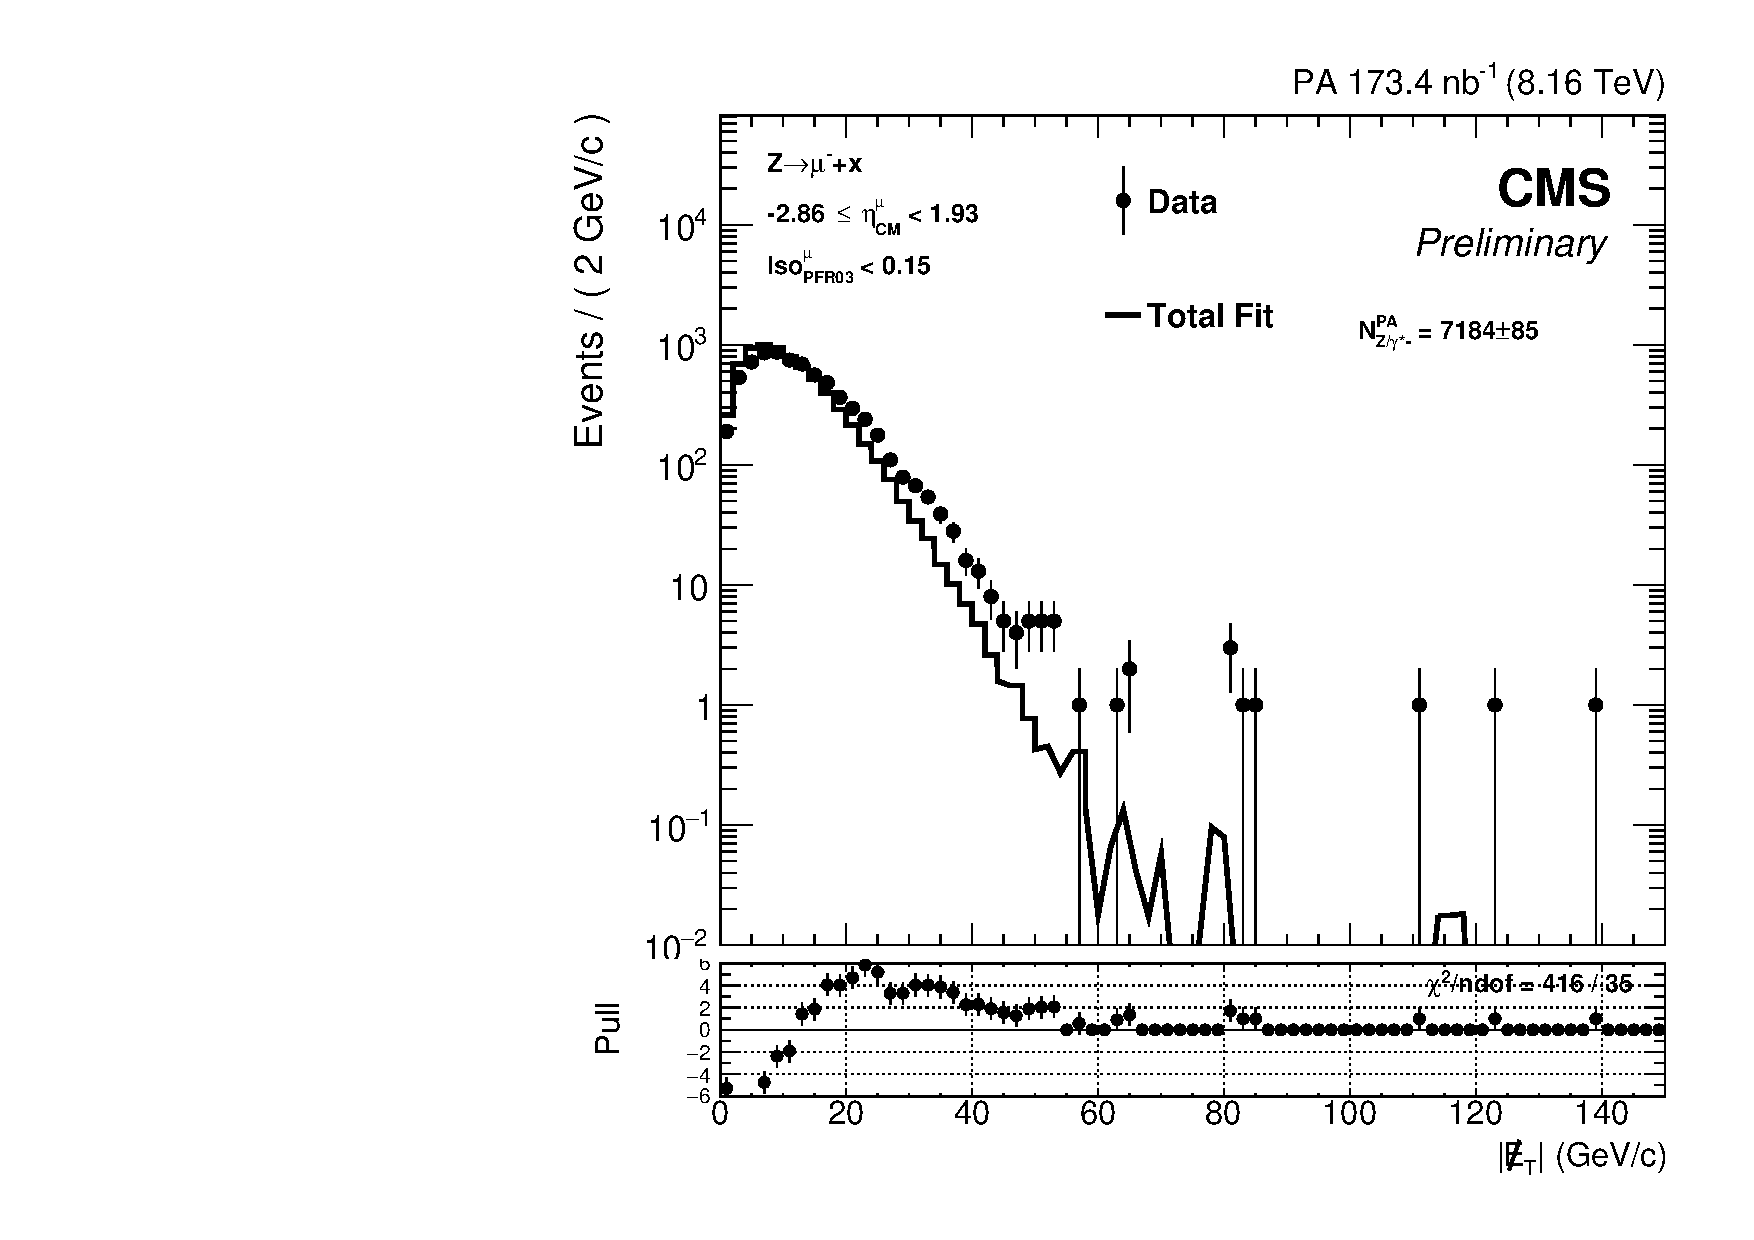
\includegraphics[width=0.4\textwidth]{Figures/WBoson/Analysis/Correction/Recoil/CheckFits/Z/METPF_RAW/PLOT_MET_DATA_ZToMuMi_PA_Model_TEMP_DY_MuEtaCM_m286_193_MuIso_0_15.pdf}
  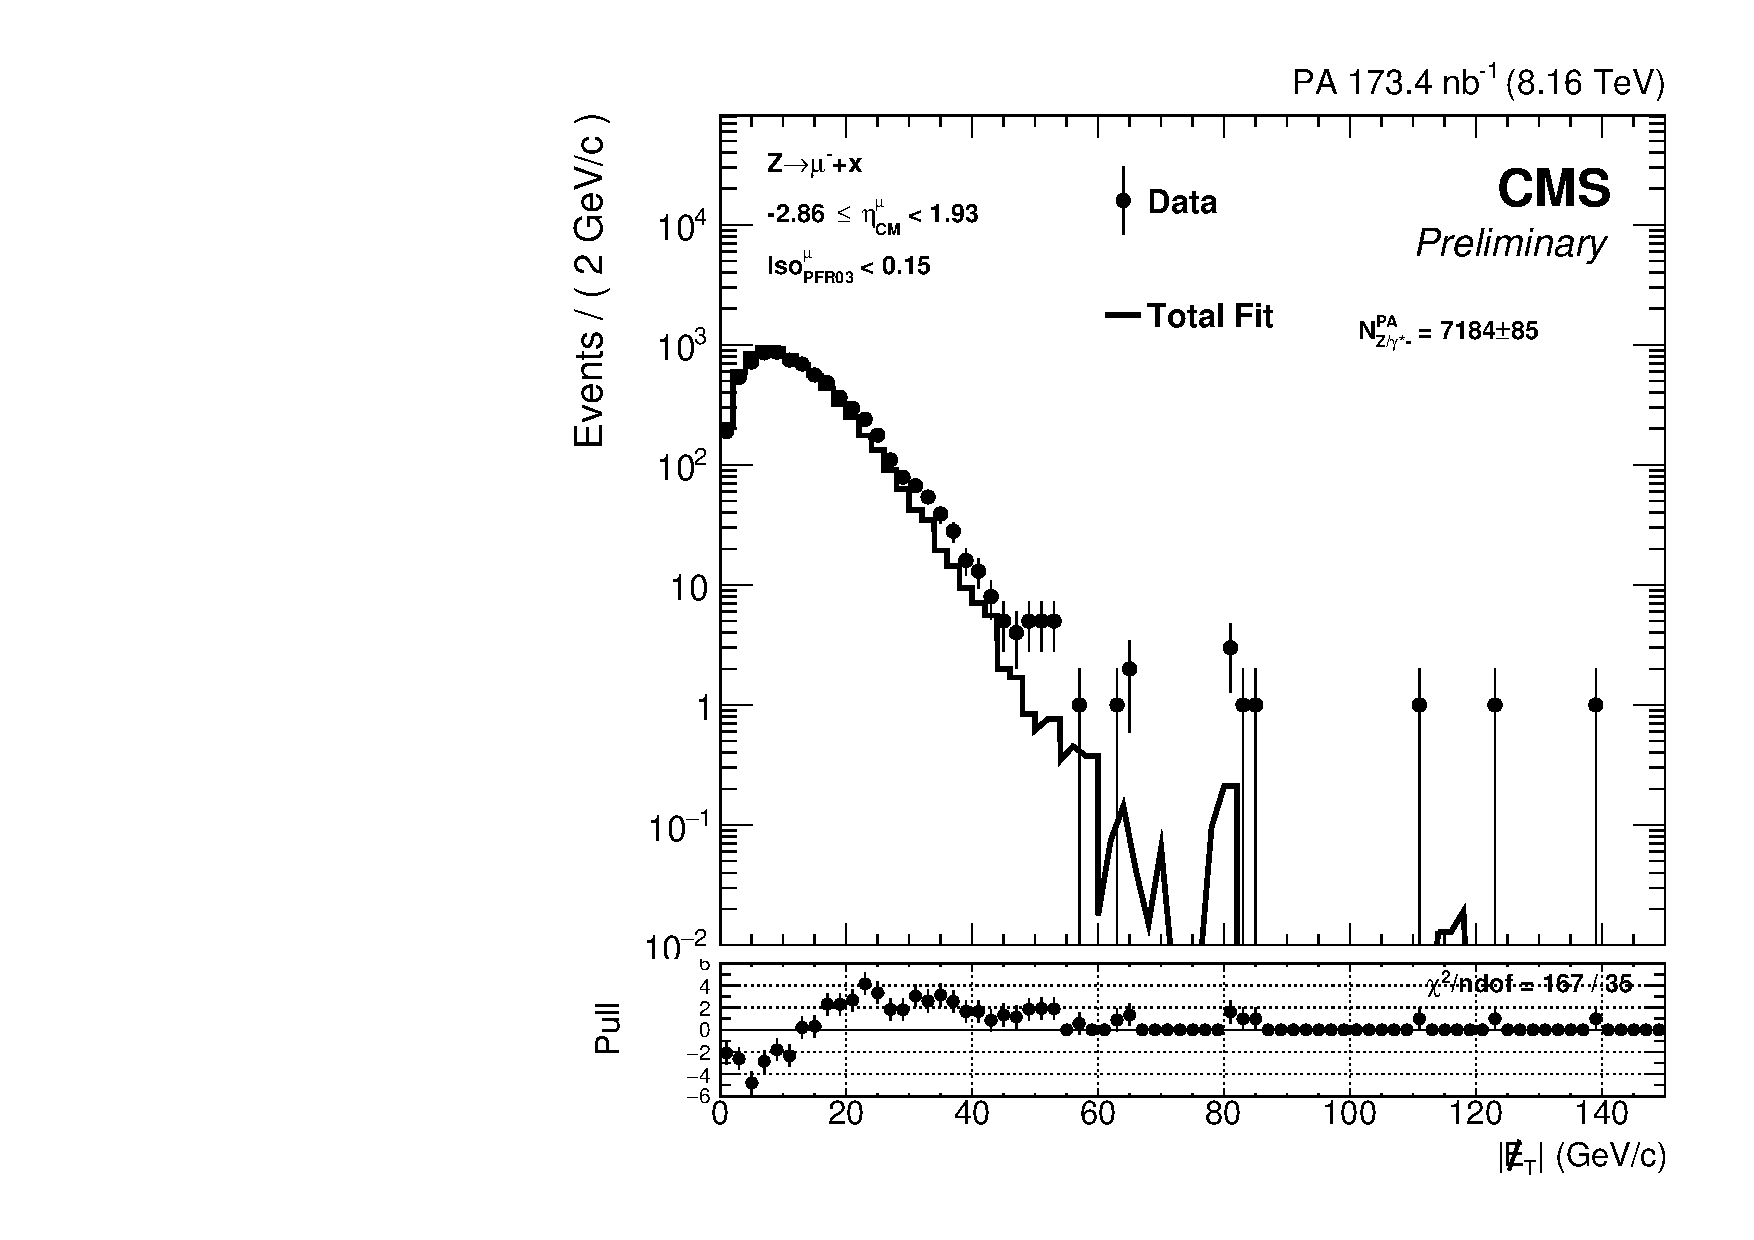
\includegraphics[width=0.4\textwidth]{Figures/WBoson/Analysis/Correction/Recoil/CheckFits/Z/METPF_RAW_HFrew/PLOT_MET_DATA_ZToMuMi_PA_Model_TEMP_DY_MuEtaCM_m286_193_MuIso_0_15.pdf} \\
  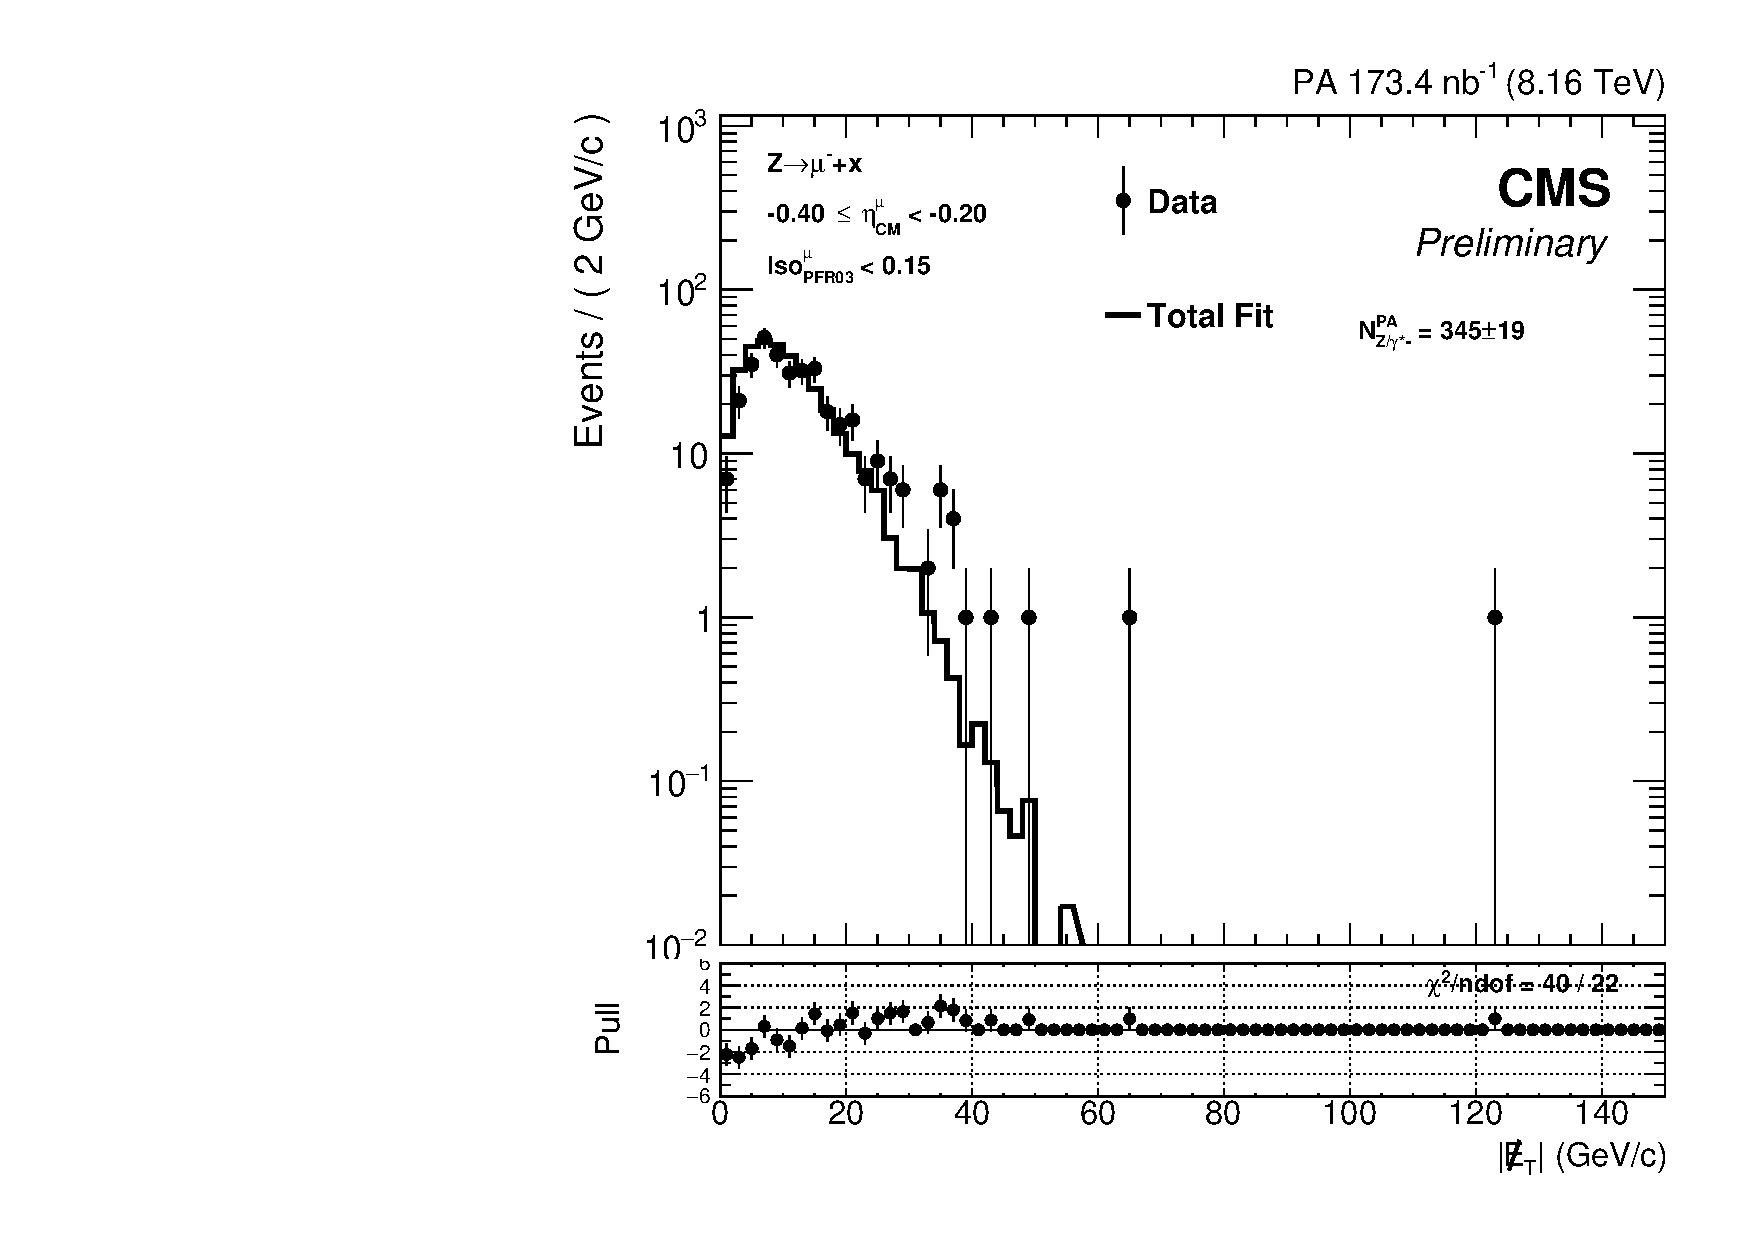
\includegraphics[width=0.4\textwidth]{Figures/WBoson/Analysis/Correction/Recoil/CheckFits/Z/METPF_RAW/PLOT_MET_DATA_ZToMuMi_PA_Model_TEMP_DY_MuEtaCM_m40_m20_MuIso_0_15.pdf}
  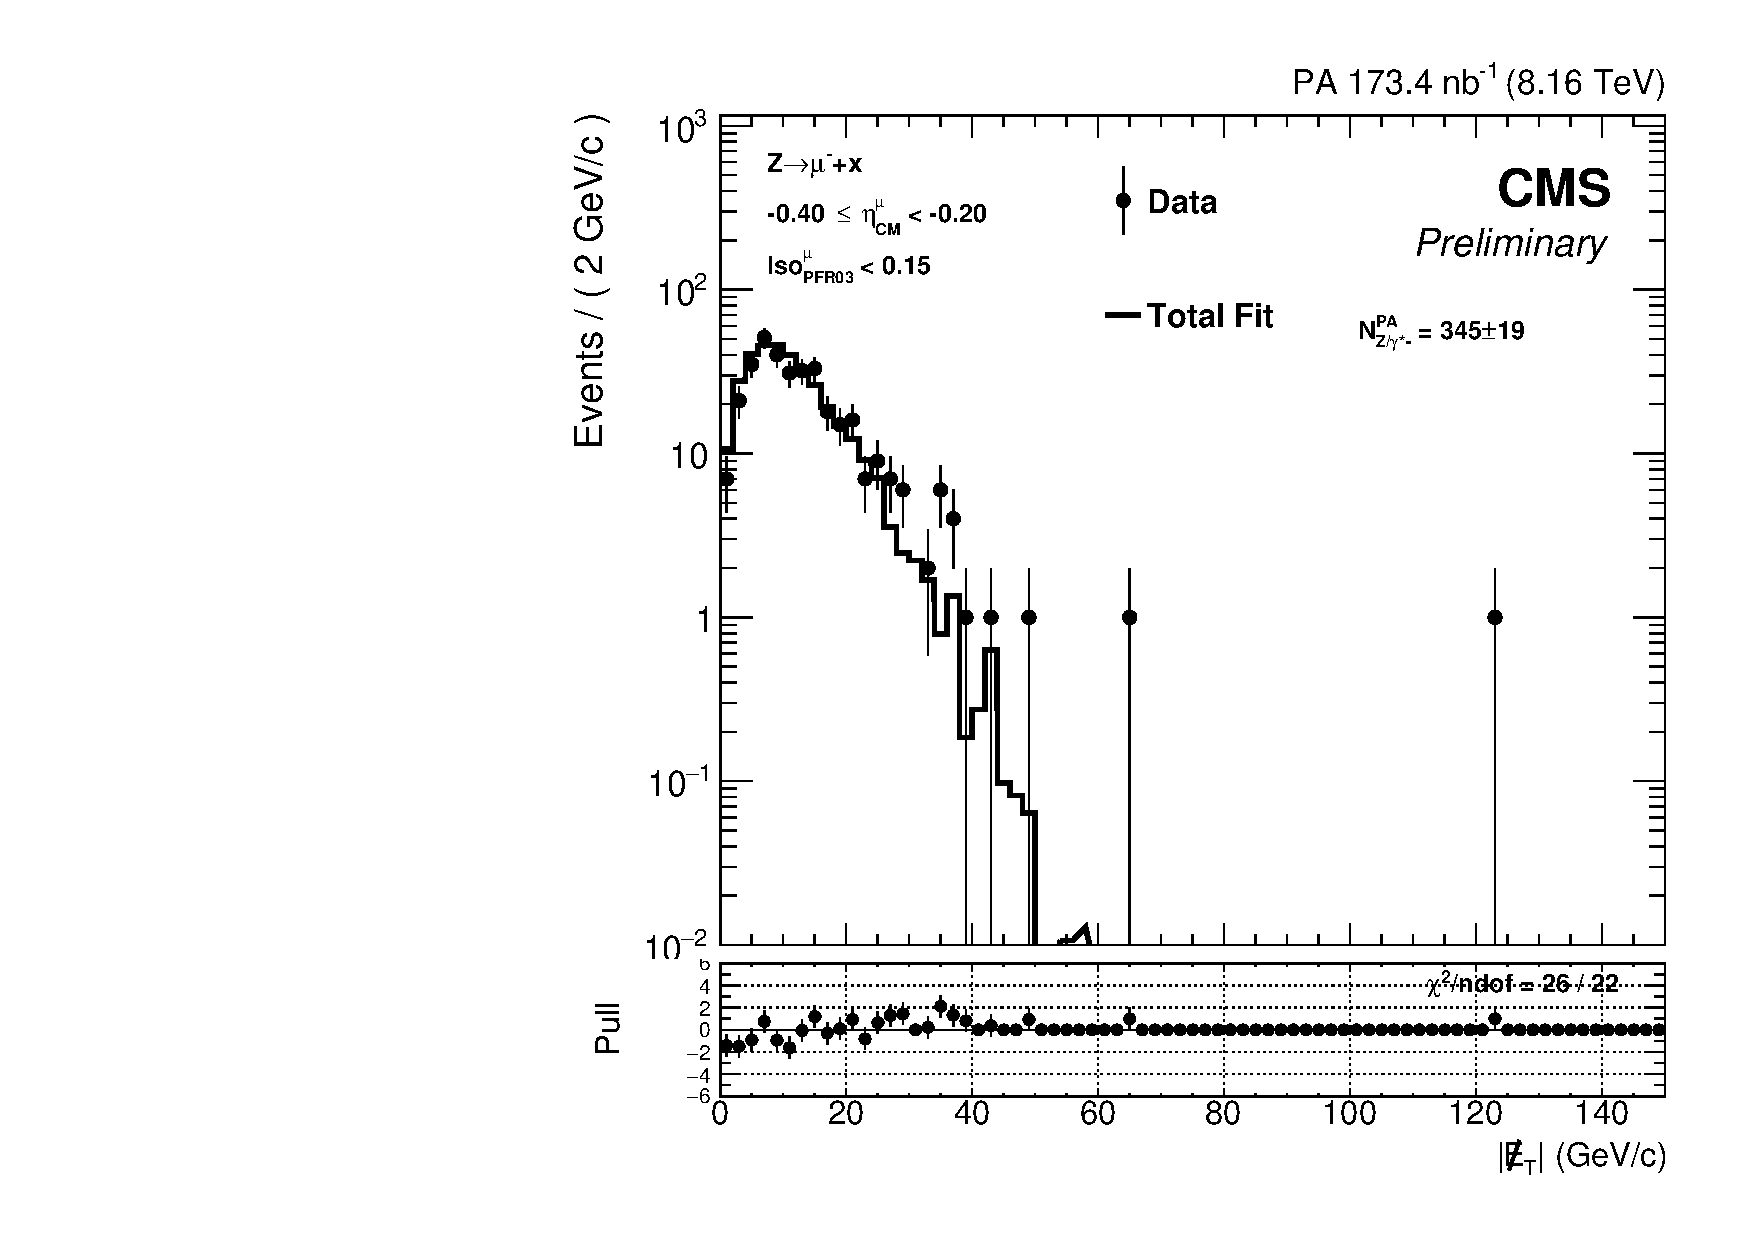
\includegraphics[width=0.4\textwidth]{Figures/WBoson/Analysis/Correction/Recoil/CheckFits/Z/METPF_RAW_HFrew/PLOT_MET_DATA_ZToMuMi_PA_Model_TEMP_DY_MuEtaCM_m40_m20_MuIso_0_15.pdf}
  \caption{A comparison of the MET distribution in data and MC for Z boson selected events. The top plots correspond to the full pseudorapidity range in the analysis while the bottom ones correspond to an specific pseudorapidity bin. The left plots use the PF MET RAW without HF reweighting in MC, while the right ones the MC events are reweighed.}
 \label{fig:HFrewCheck}
 \end{center}
\end{figure}


\subsection{Corrections for MET} \label{sec:WBoson_Corrections_MET}

As mentioned in \sect{sec:WBoson_Selection_MET}, the MET is defined as the sum of the \pt of all the particles reconstructed with the PF algorithm, including those produced by the underlying events. Therefore, the first step to improve the simulation of the MET consist of correcting the modelling of the event activity from the EPOS minimum bias events by reweighing the HF energy distribution as explained in \sect{sec:WBoson_Corrections_EventActivityReweighing}. The low MET region in MC agrees better with the data distribution after applying the HF energy reweighing.

The width of the MET distribution in \ZToMuMu events represents the MET resolution due to the \pt measurement of the PF particles. Differences in the emulation of the detector conditions is one of the main sources of disagreement between simulation and data in the high MET region of a \Z boson enriched sample. The simulated MET resolution describes better the data after correcting the hadronic recoil present in MC events.

\subsection{Definition of recoil} \label{sec:WBoson_Corrections_RecoilCorrection}

The hadronic recoil of \ZToMuMu events is defined as the vector sum of the \pt of all PF candidates excluding the muons from the boson decay. Considering the definition of MET, the recoil vector can be expressed as:

\begin{equation}\label{eq:equT} 
\vec{u}_{T} = -\VETslash\ \ - \vec{q}_{T},
\end{equation}

where $\vec{u}_{T}$ is the hadronic recoil in the transverse plane to the beam direction and $\vec{q}_{T}$ is the transverse momentum of the \Z boson.

In the case of \WToMuNu events, the recoil is defined as:

\begin{equation}\label{eq:equTW}
\vec{u}_{T} = -\VETslash\ \ - \vec{p}_{T}^{\mu},
\end{equation}

where $\vec{p}_{T}^{\mu}$ is the \pt of the muon.

The recoil vector is projected along the transverse plane in the boson direction. The parallel and perpendicular components of the recoil vector with respect to the boson $\vec{q}_{T}$ are labelled as $u_{\parallel}$ and $u_{\perp}$, respectively. \fig{fig:RecoilDefinition} describes the recoil and its components.

\begin{figure}
 \begin{center}
  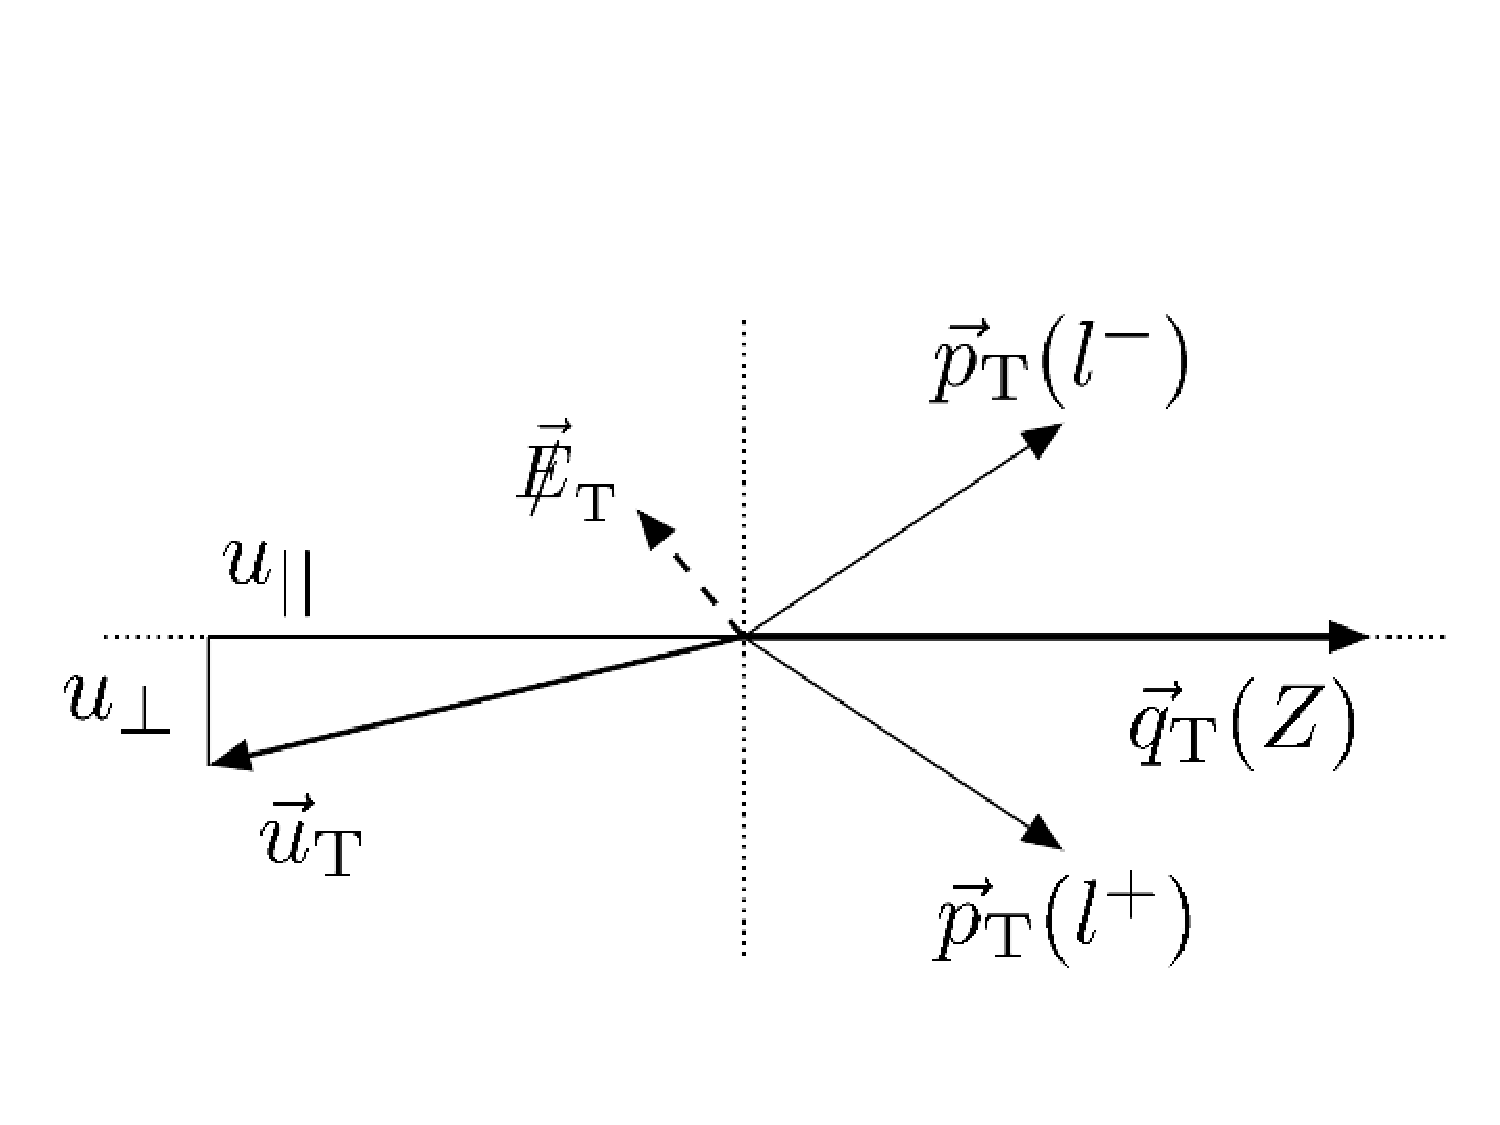
\includegraphics[width=0.4\textwidth]{Figures/WBoson/Analysis/Correction/Recoil/Recoil_Definition.pdf}
  \caption{Definition of the recoil vector and its components for \ZToMuMu events.}
  \label{fig:RecoilDefinition}
 \end{center}
\end{figure}
 
The boson transverse momentum vector $\vec{q}_{T}$ is determined in MC using the reconstructed decay products whenever possible. In the \WToMuNu MC samples, the $\vec{q}_{T}$ is derived from the sum of the \pt of the reconstructed muon and the generated neutrino, while for the \WToTauNu, \DYToTauTau and \ttbar, the $\vec{q}_{T}$ is taken from the generated boson \pt. In the case of \DYToMuMu, if the sub-leading muon falls outside of the coverage of the CMS detector, the \Z boson $q_{T}$ is computed from the sum of the reconstructed leading muon \pt and the generated sub-leading muon \pt, otherwise the $q_{T}$ is equal to the sum of both reconstructed muons \pt.

The recoil corrections are extracted using a \Z control sample. In order to compute them, the parallel and perpendicular components of the recoil vector are determined event by event in data and MC, and their distributions are sorted in bins of $q_{T}$. The recoil distributions are fitted with an unbinned maximum likelihood fit. A combination of two Gaussian functions is chosen to better describe the shape of the recoil distributions. Examples of the distributions of the parallel and perpendicular recoil components, denoted as $u_{1}$ and $u_{2}$ respectively, are shown in \fig{fig:RecoilFits} for data and simulation. Furthermore, the fits performed using the double Gaussian functions, and their corresponding pull distributions are also shown.

\begin{figure}
 \begin{center}
  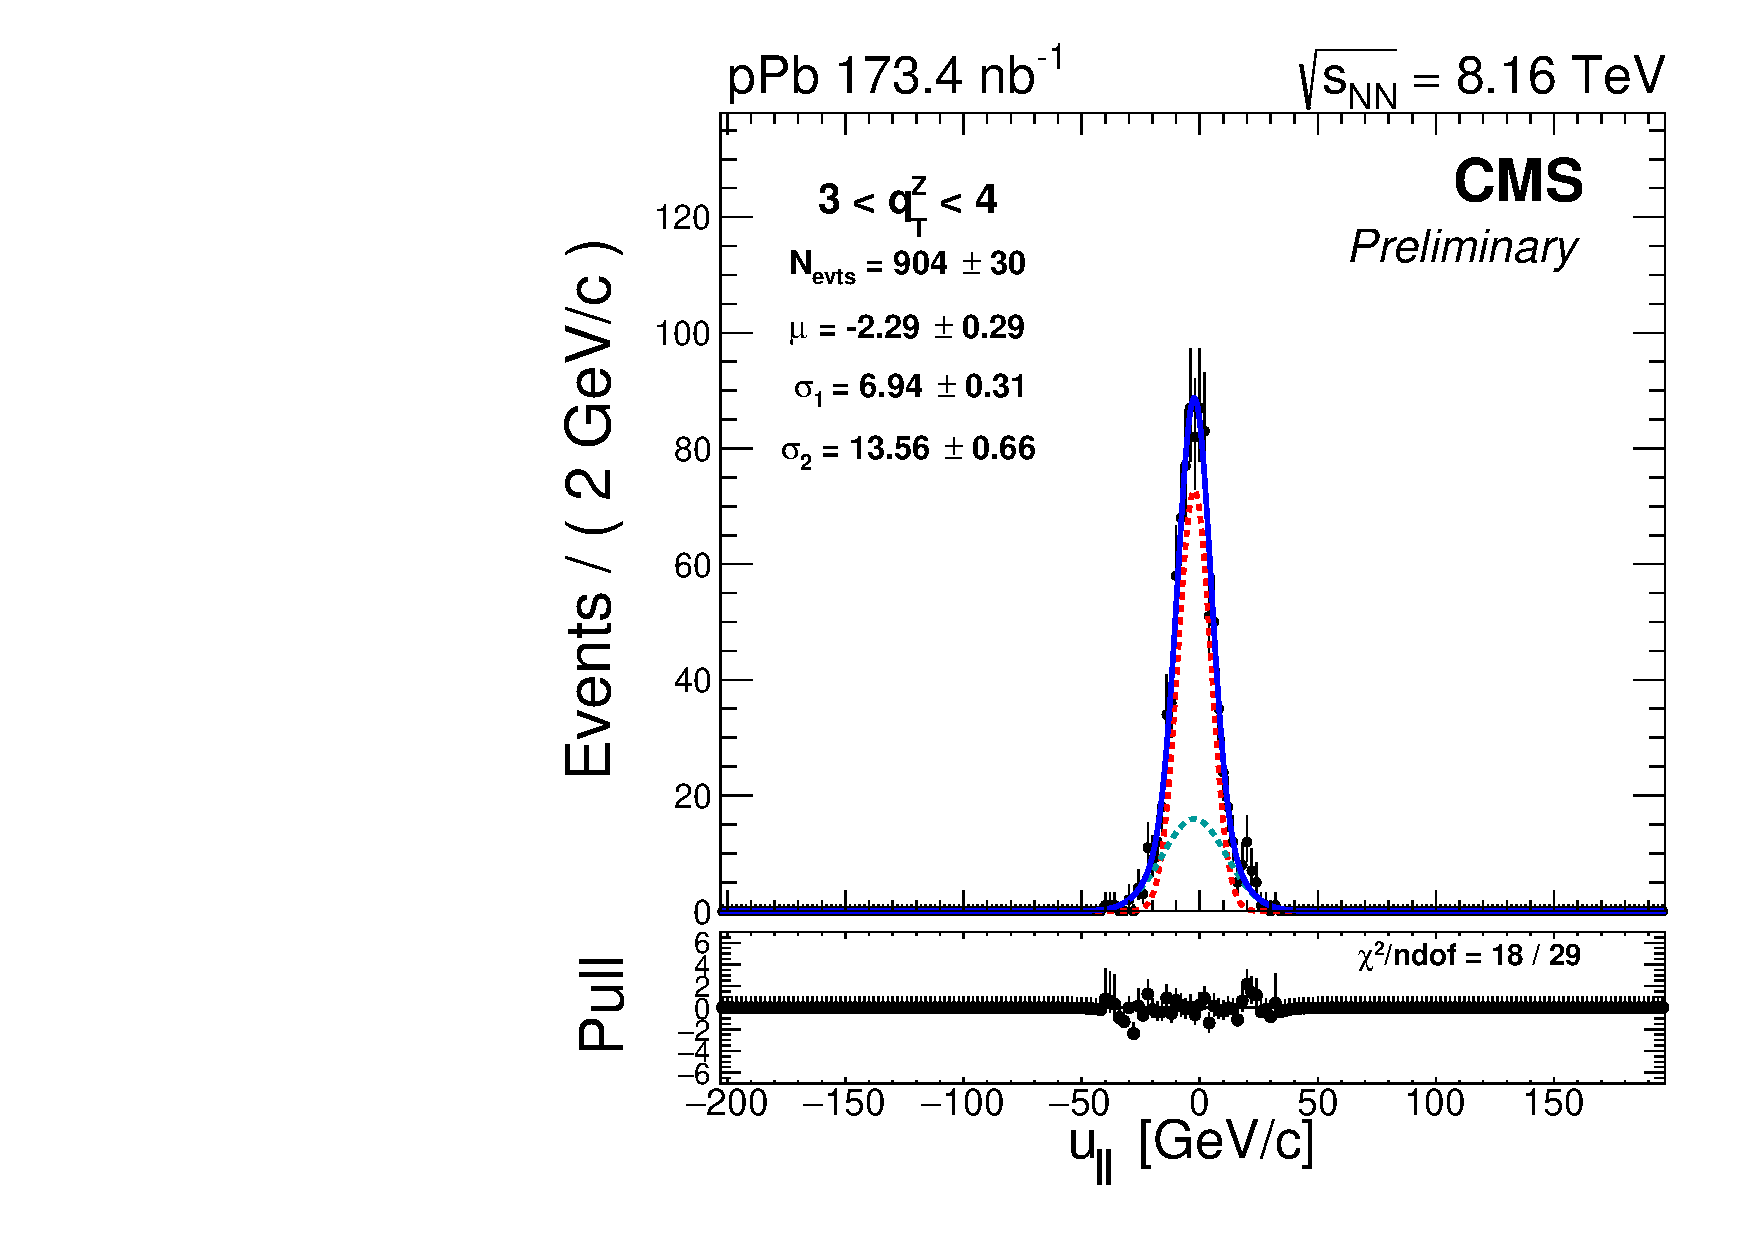
\includegraphics[width=0.4\textwidth]{Figures/WBoson/Analysis/Correction/Recoil/RecoilFits/Data/pfu1fit_2.pdf}
  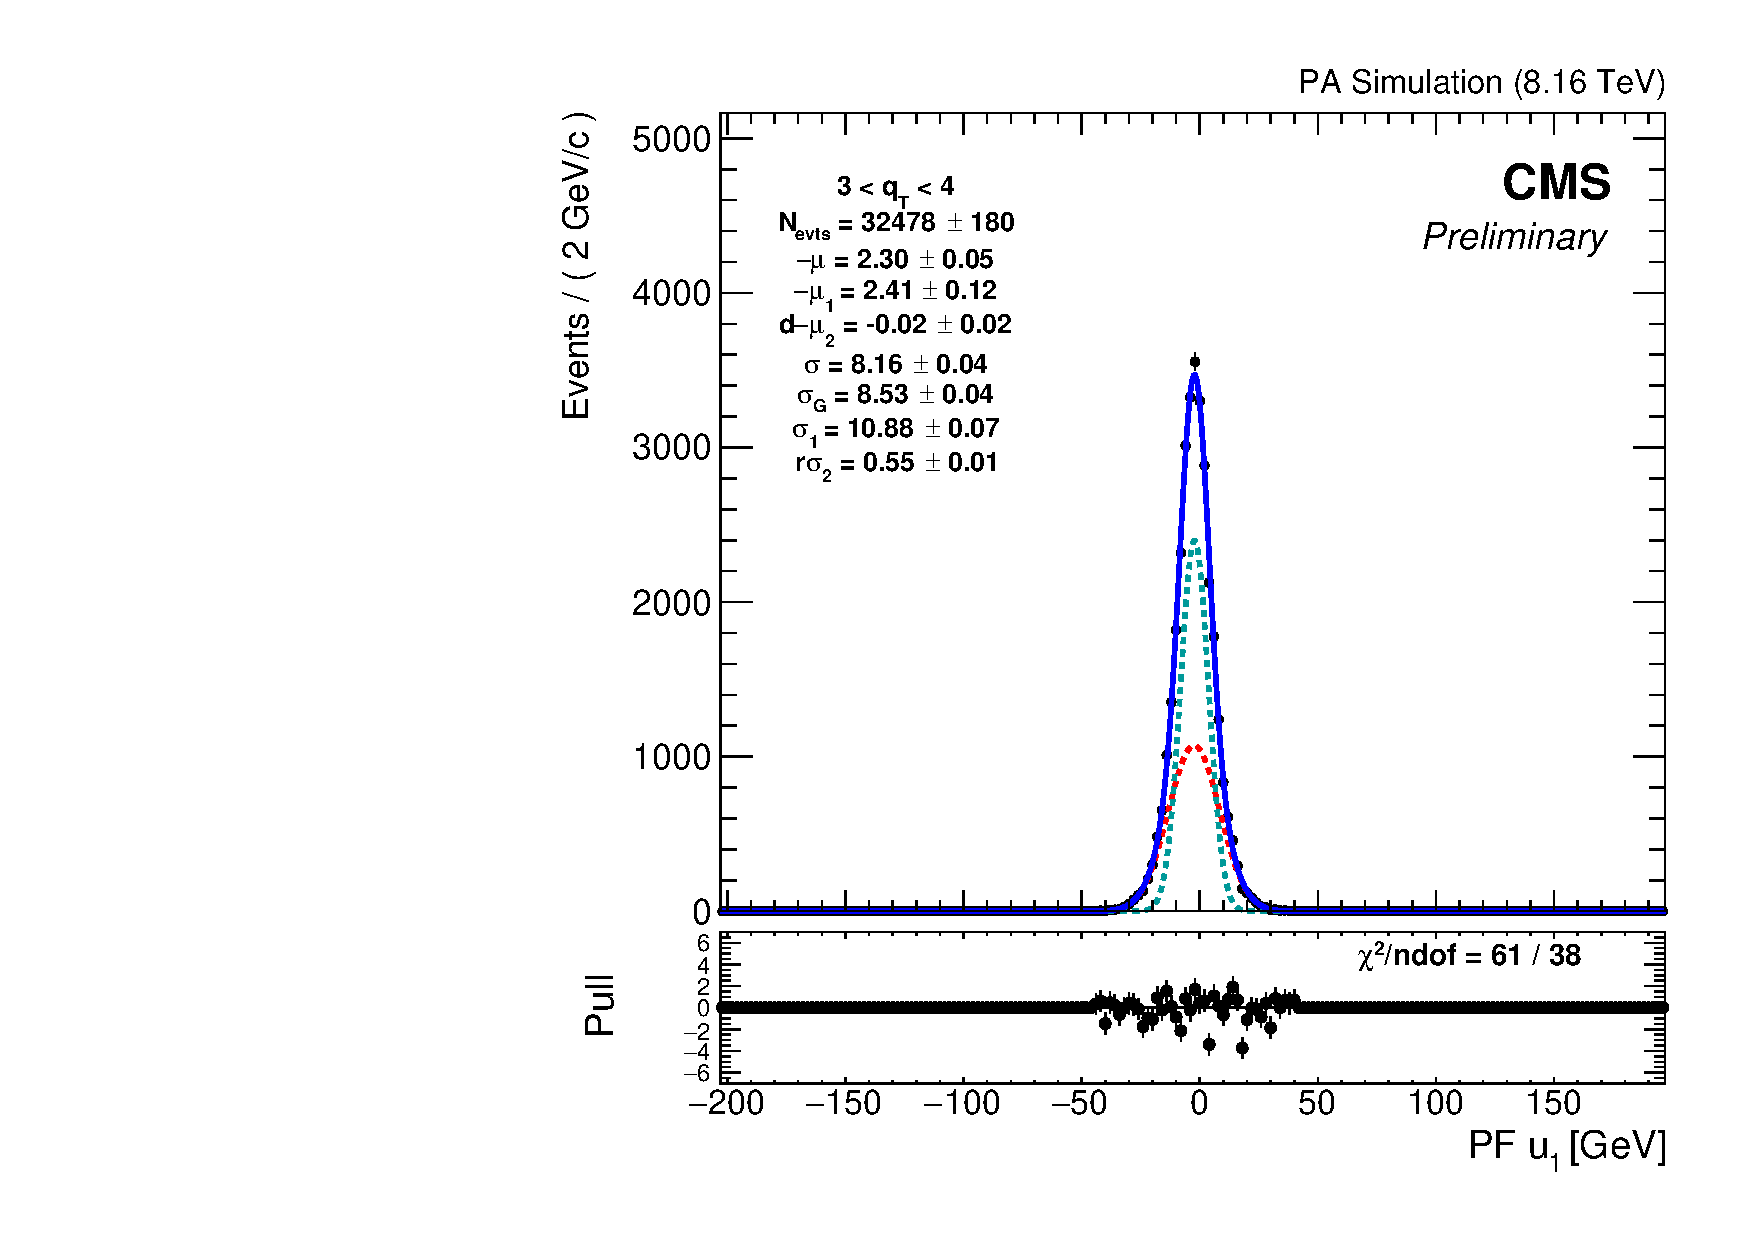
\includegraphics[width=0.4\textwidth]{Figures/WBoson/Analysis/Correction/Recoil/RecoilFits/MC/pfu1fit_2.pdf} \\
  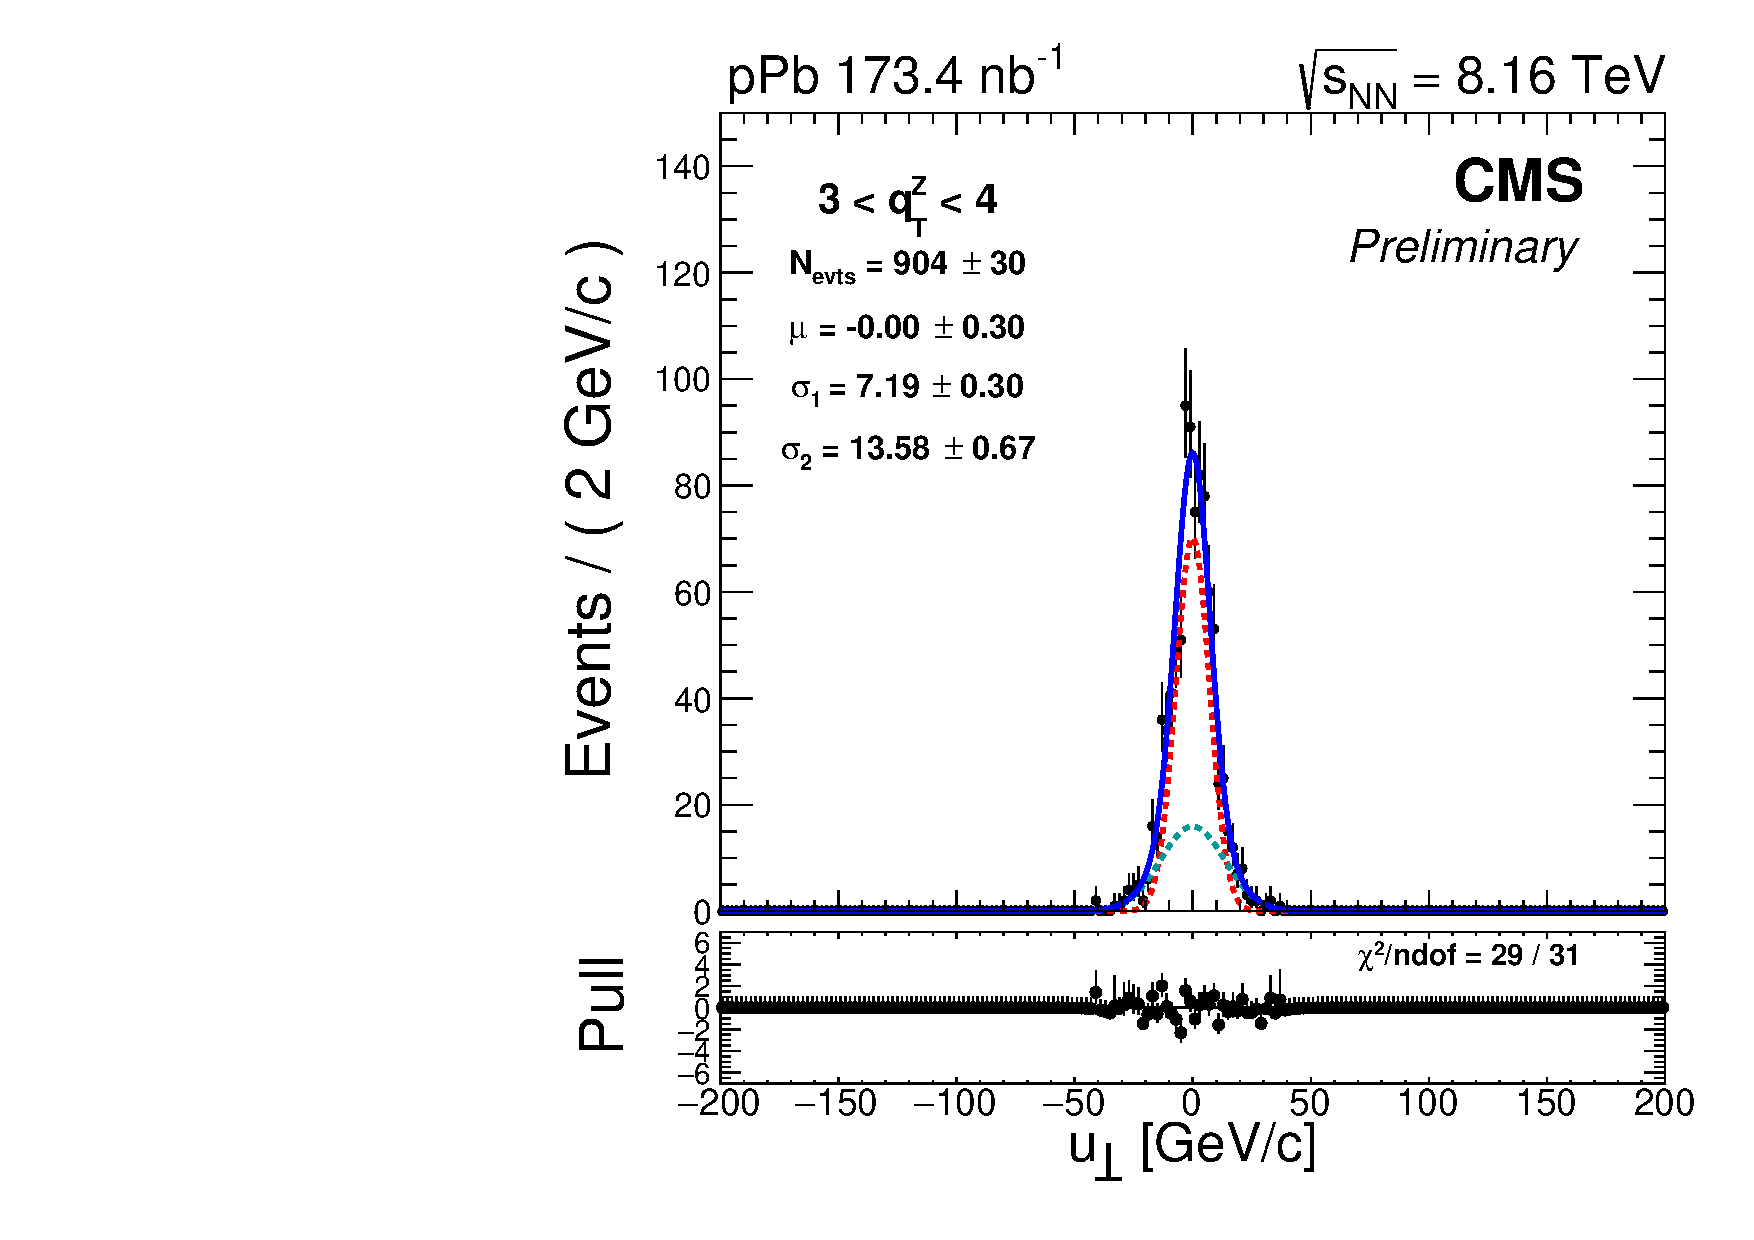
\includegraphics[width=0.4\textwidth]{Figures/WBoson/Analysis/Correction/Recoil/RecoilFits/Data/pfu2fit_2.pdf}
  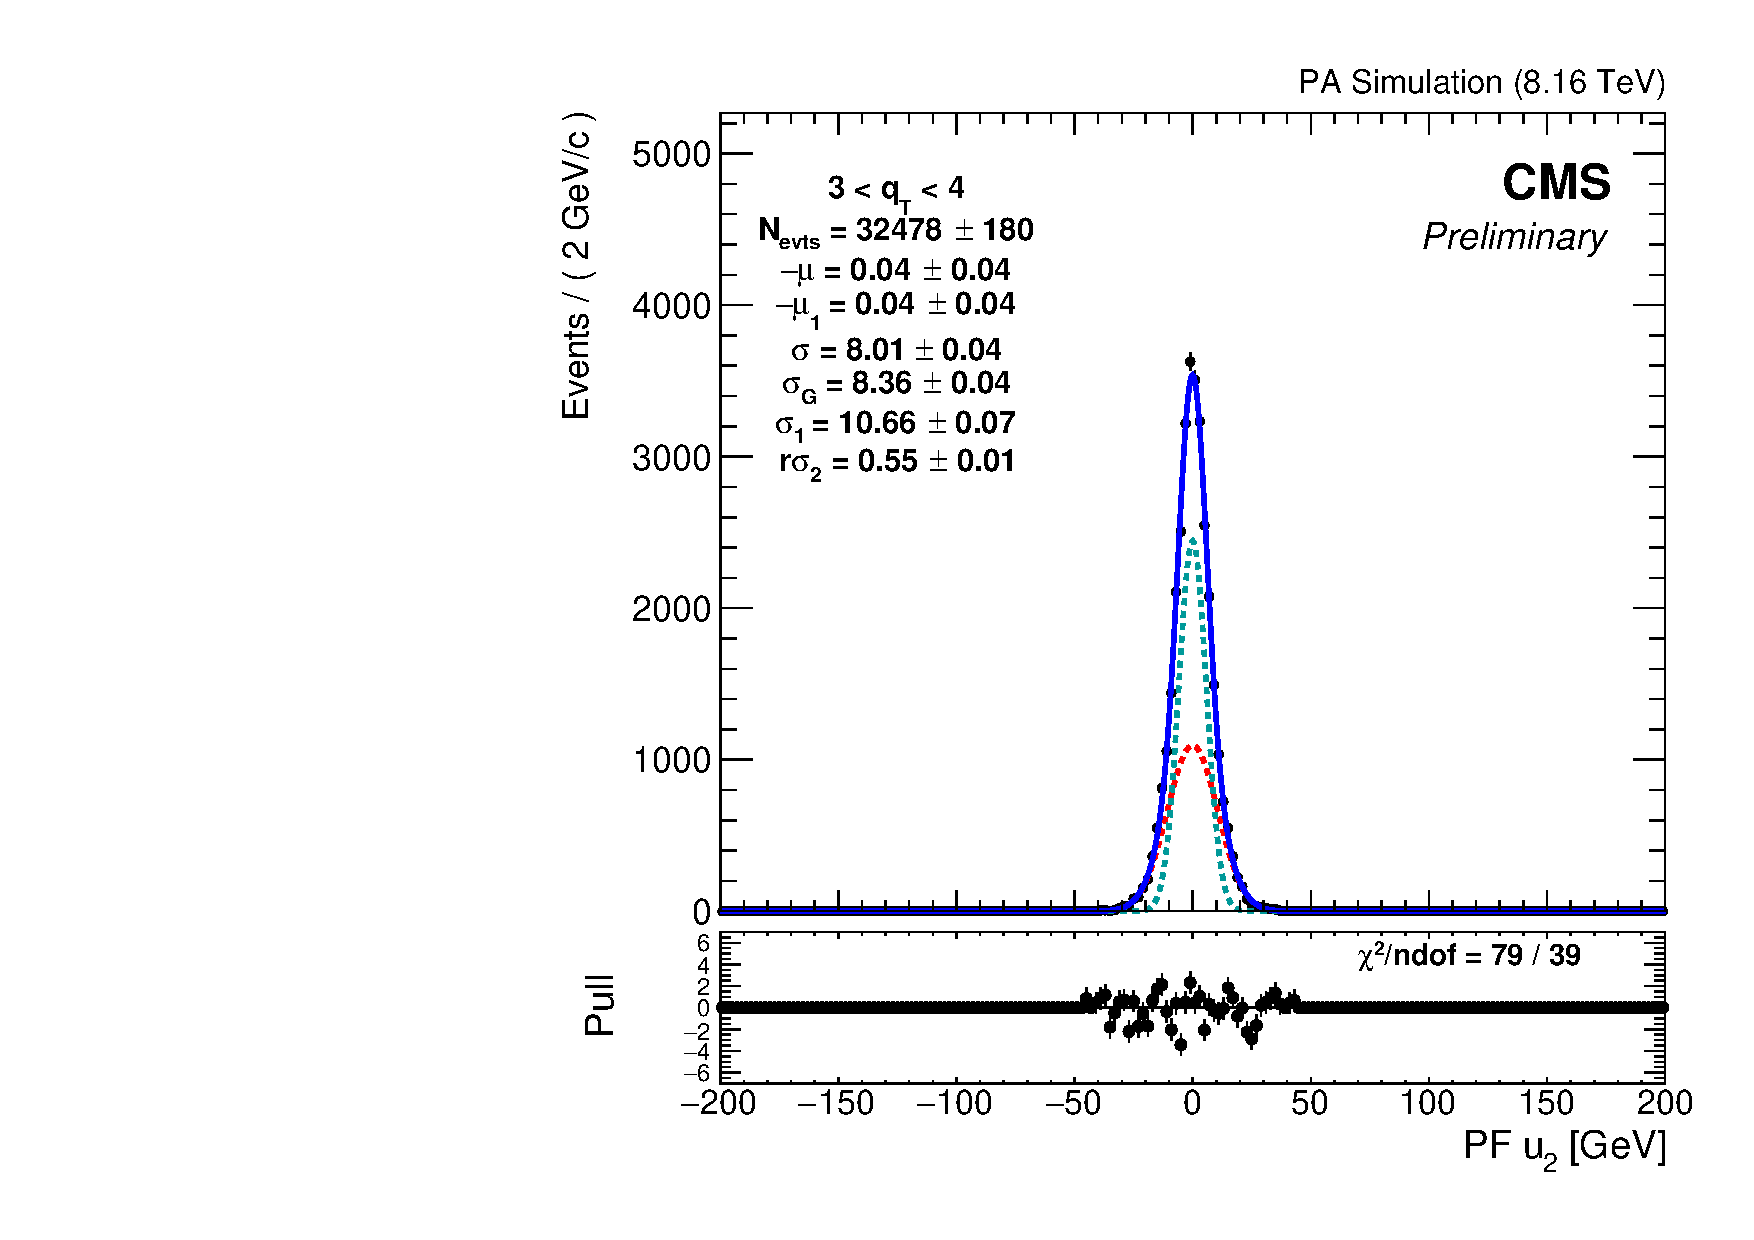
\includegraphics[width=0.4\textwidth]{Figures/WBoson/Analysis/Correction/Recoil/RecoilFits/MC/pfu2fit_2.pdf}
  \caption{Distributions of the parallel (top) and perpendicular (bottom) components of the recoil in data (left) and MC (right). The fit function is based on a weighted sum of two Gaussian distributions. The plots correspond to the $q_{T}$ bin [3, 4]~GeV.}
 \label{fig:RecoilFits}
 \end{center}
\end{figure}
 
\subsubsection{Recoil Scale}\label{sec:WBoson_Corrections_MET_Rscale}

The mean pamareters ($\mu_{1}$ and $\mu_{2}$) of the parallel component of the recoil ($u_{1}$) are extracted in different bins of $q_{T}$ by fitting the recoil distribution as shown in \fig{fig:RecoilFits}. Afterwards, the profile of the average recoil as a function of $q_{T}$ is fitted using the following function: 

\begin{equation}\label{eq:equparparam} 
-\mu_{1,2}(q_{T}) = (c_{0} + c_{1}q_{T})(1 + erf(\alpha q_{T}^{\beta}))
\end{equation}

The fits of the average values of the parallel component of the recoil versus $q_{T}$ are shown in \fig{fig:figU1RecoilScaleFit}. In addition, the average mean value given by $\mu = f \cdot \mu_{1} + (1 - f) \cdot \mu_{2}$, is also shown. The difference between data and the simulation as a function of $q_{T}$ is used on an event by event basis to correct the scale of the recoil in MC.

\begin{figure}
 \begin{center}
  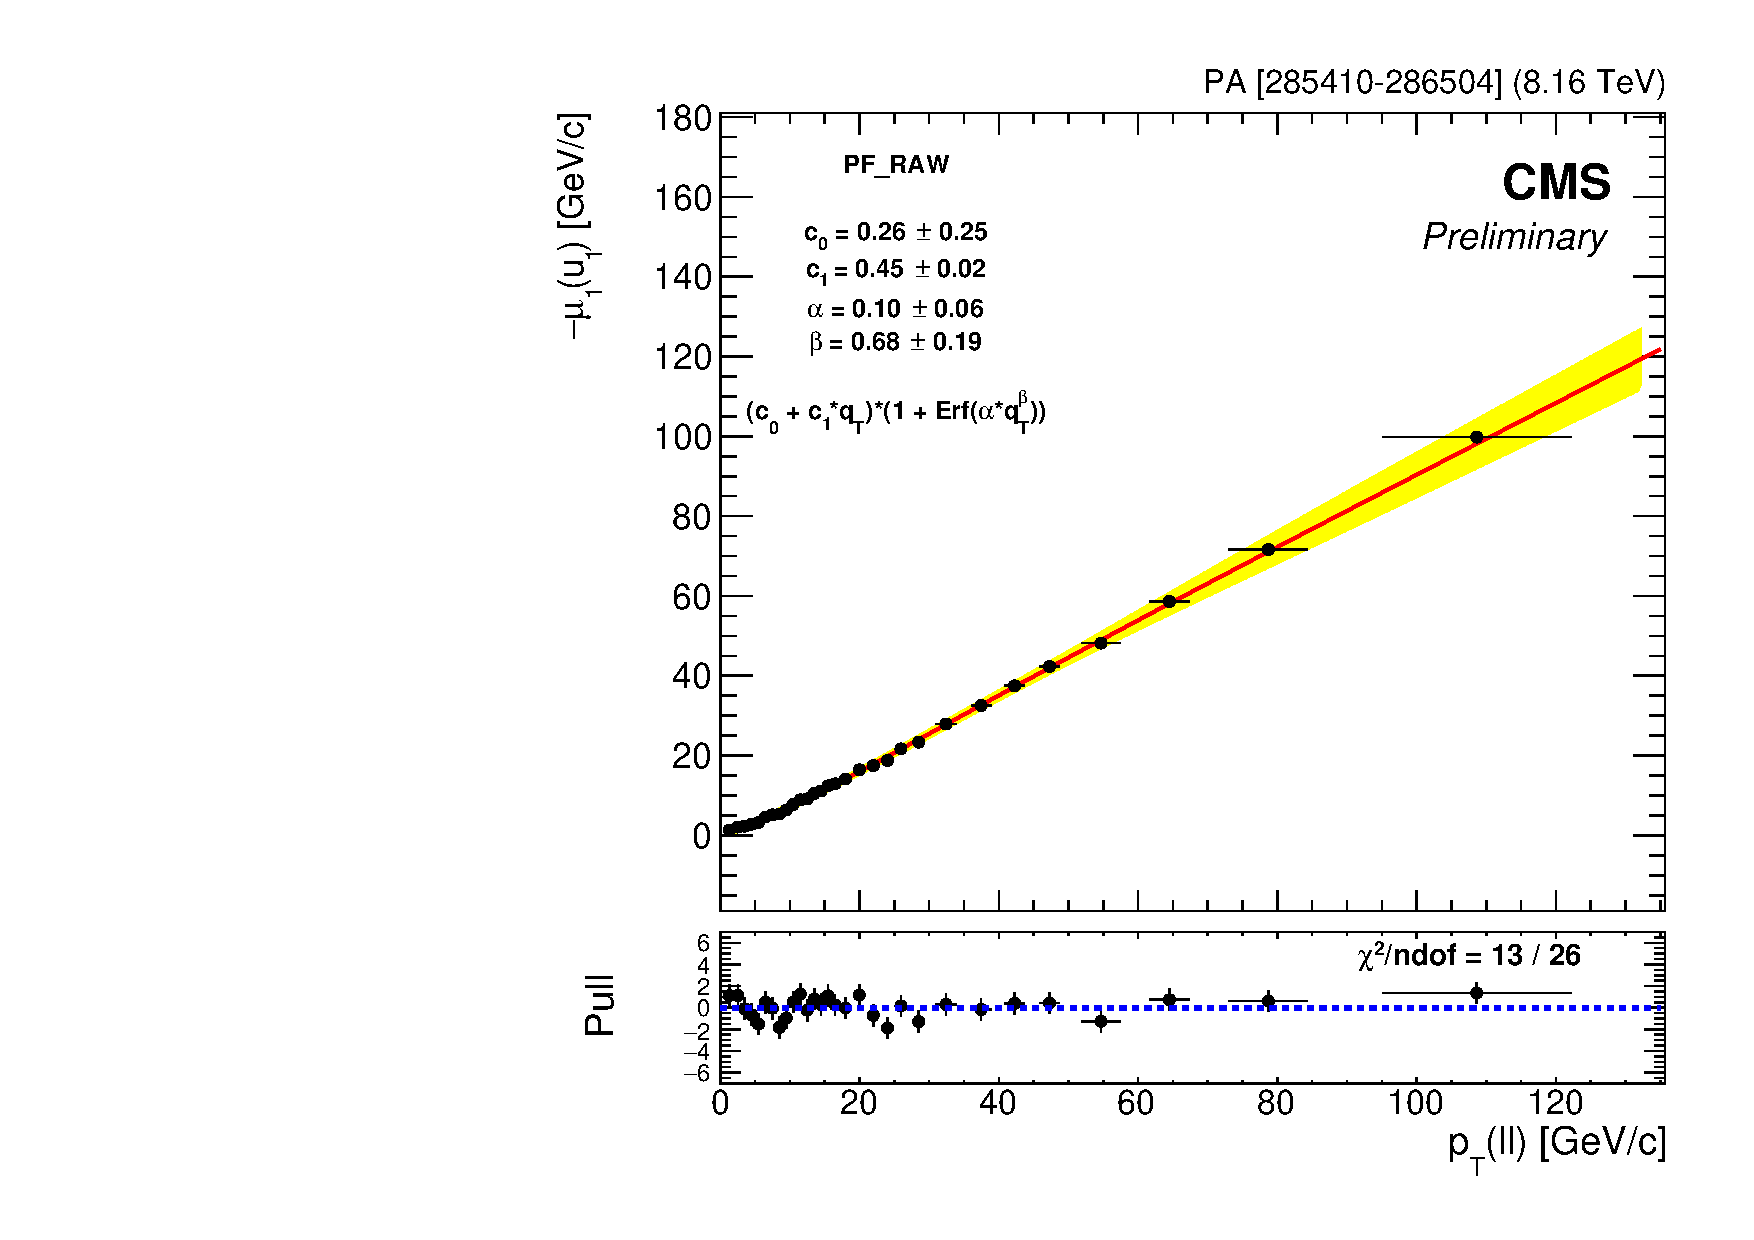
\includegraphics[width=0.3\textwidth]{Figures/WBoson/Analysis/Correction/Recoil/RecoilFitsqT/Data/fitPFu1mean1.pdf}
  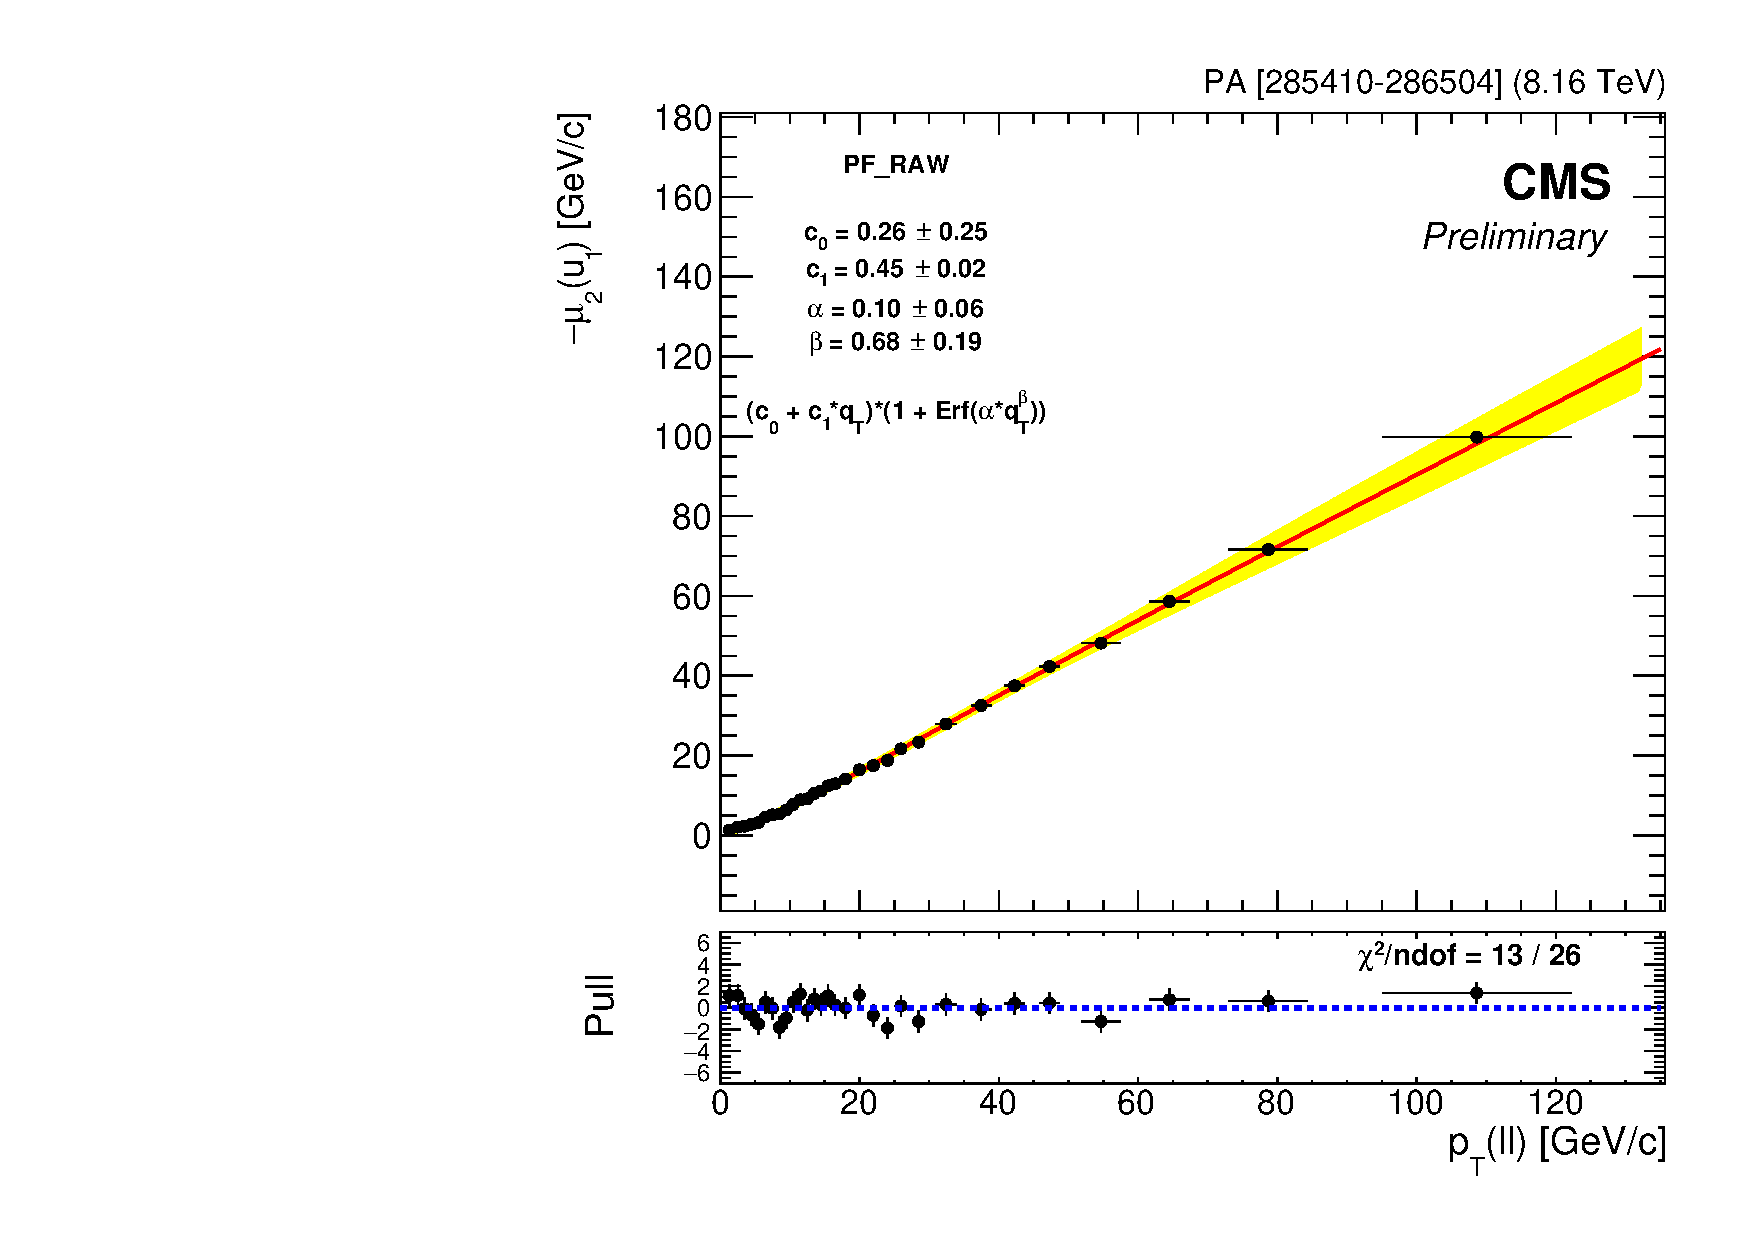
\includegraphics[width=0.3\textwidth]{Figures/WBoson/Analysis/Correction/Recoil/RecoilFitsqT/Data/fitPFu1mean2.pdf}
  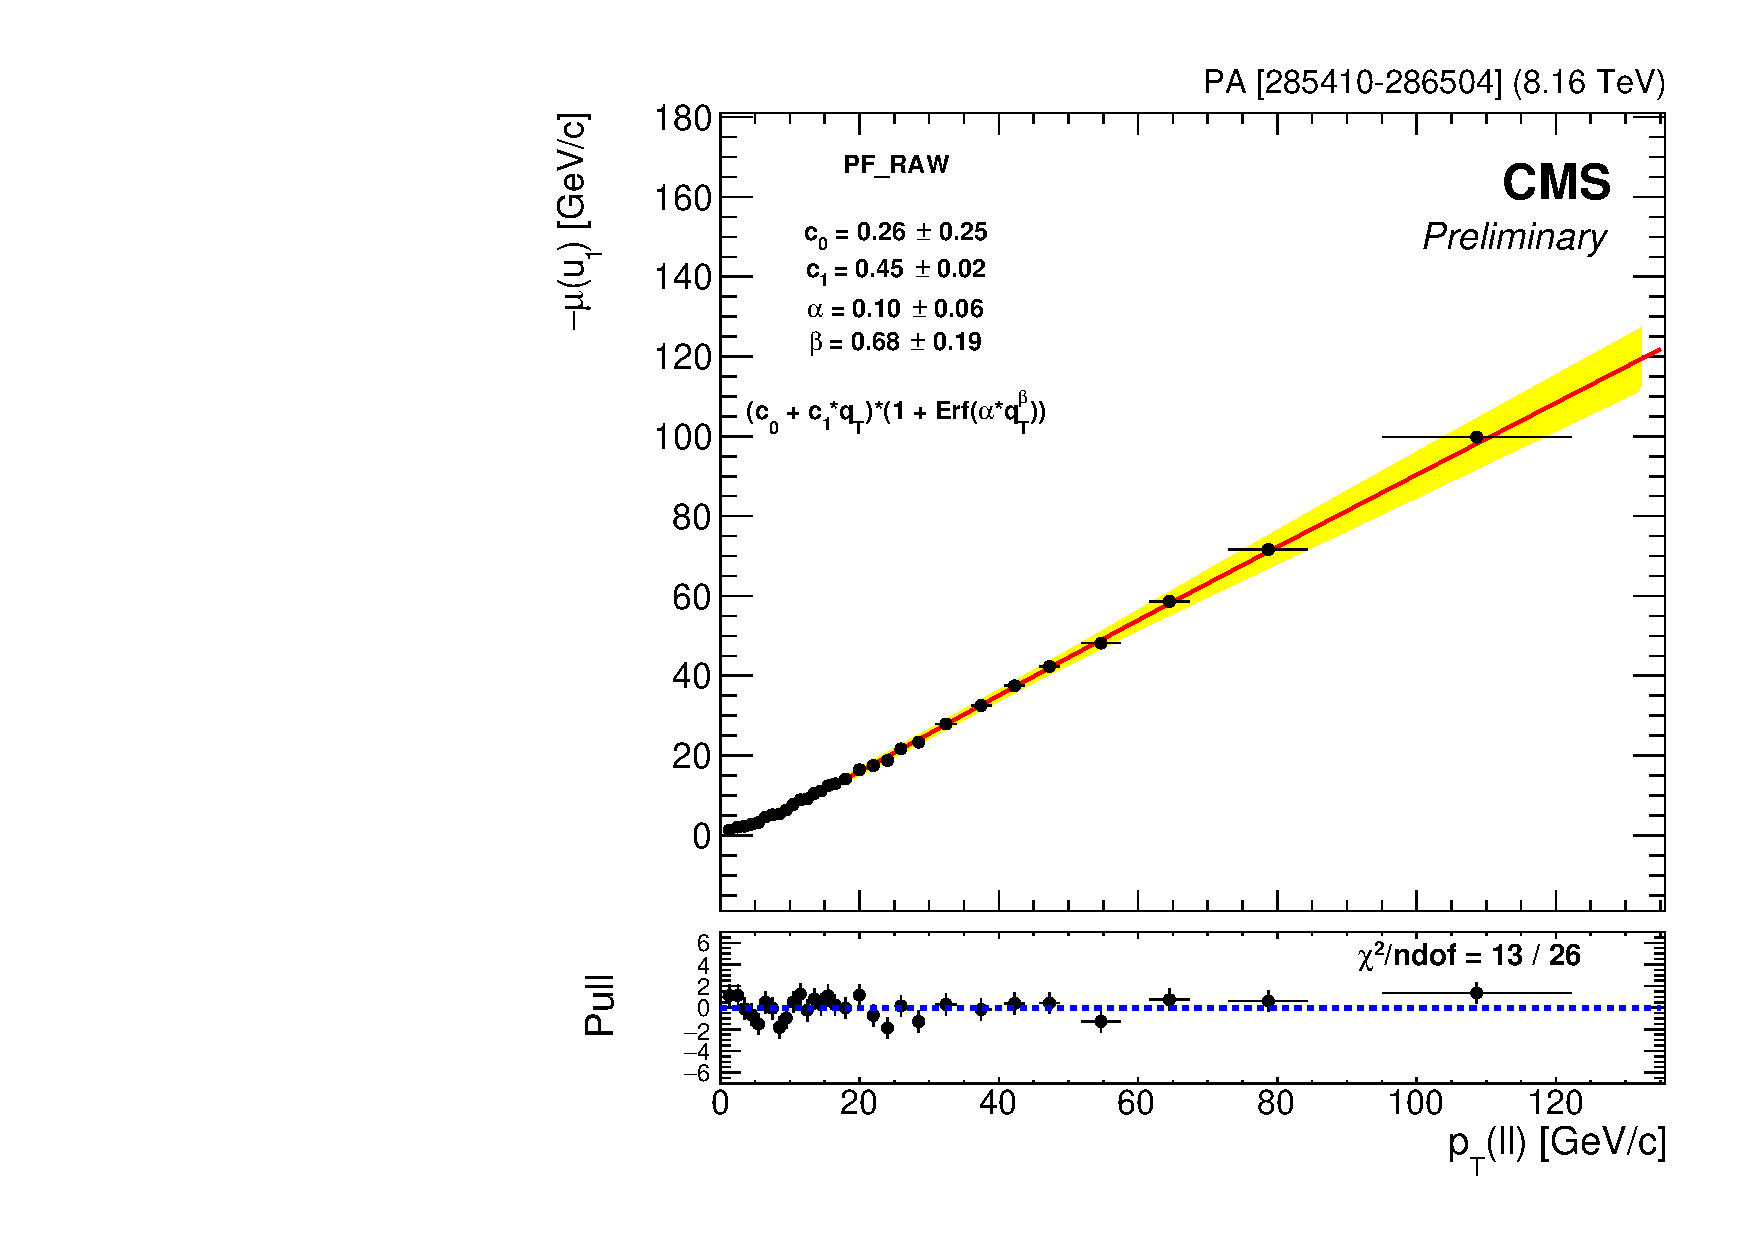
\includegraphics[width=0.3\textwidth]{Figures/WBoson/Analysis/Correction/Recoil/RecoilFitsqT/Data/fitPFu1mean.pdf} \\
  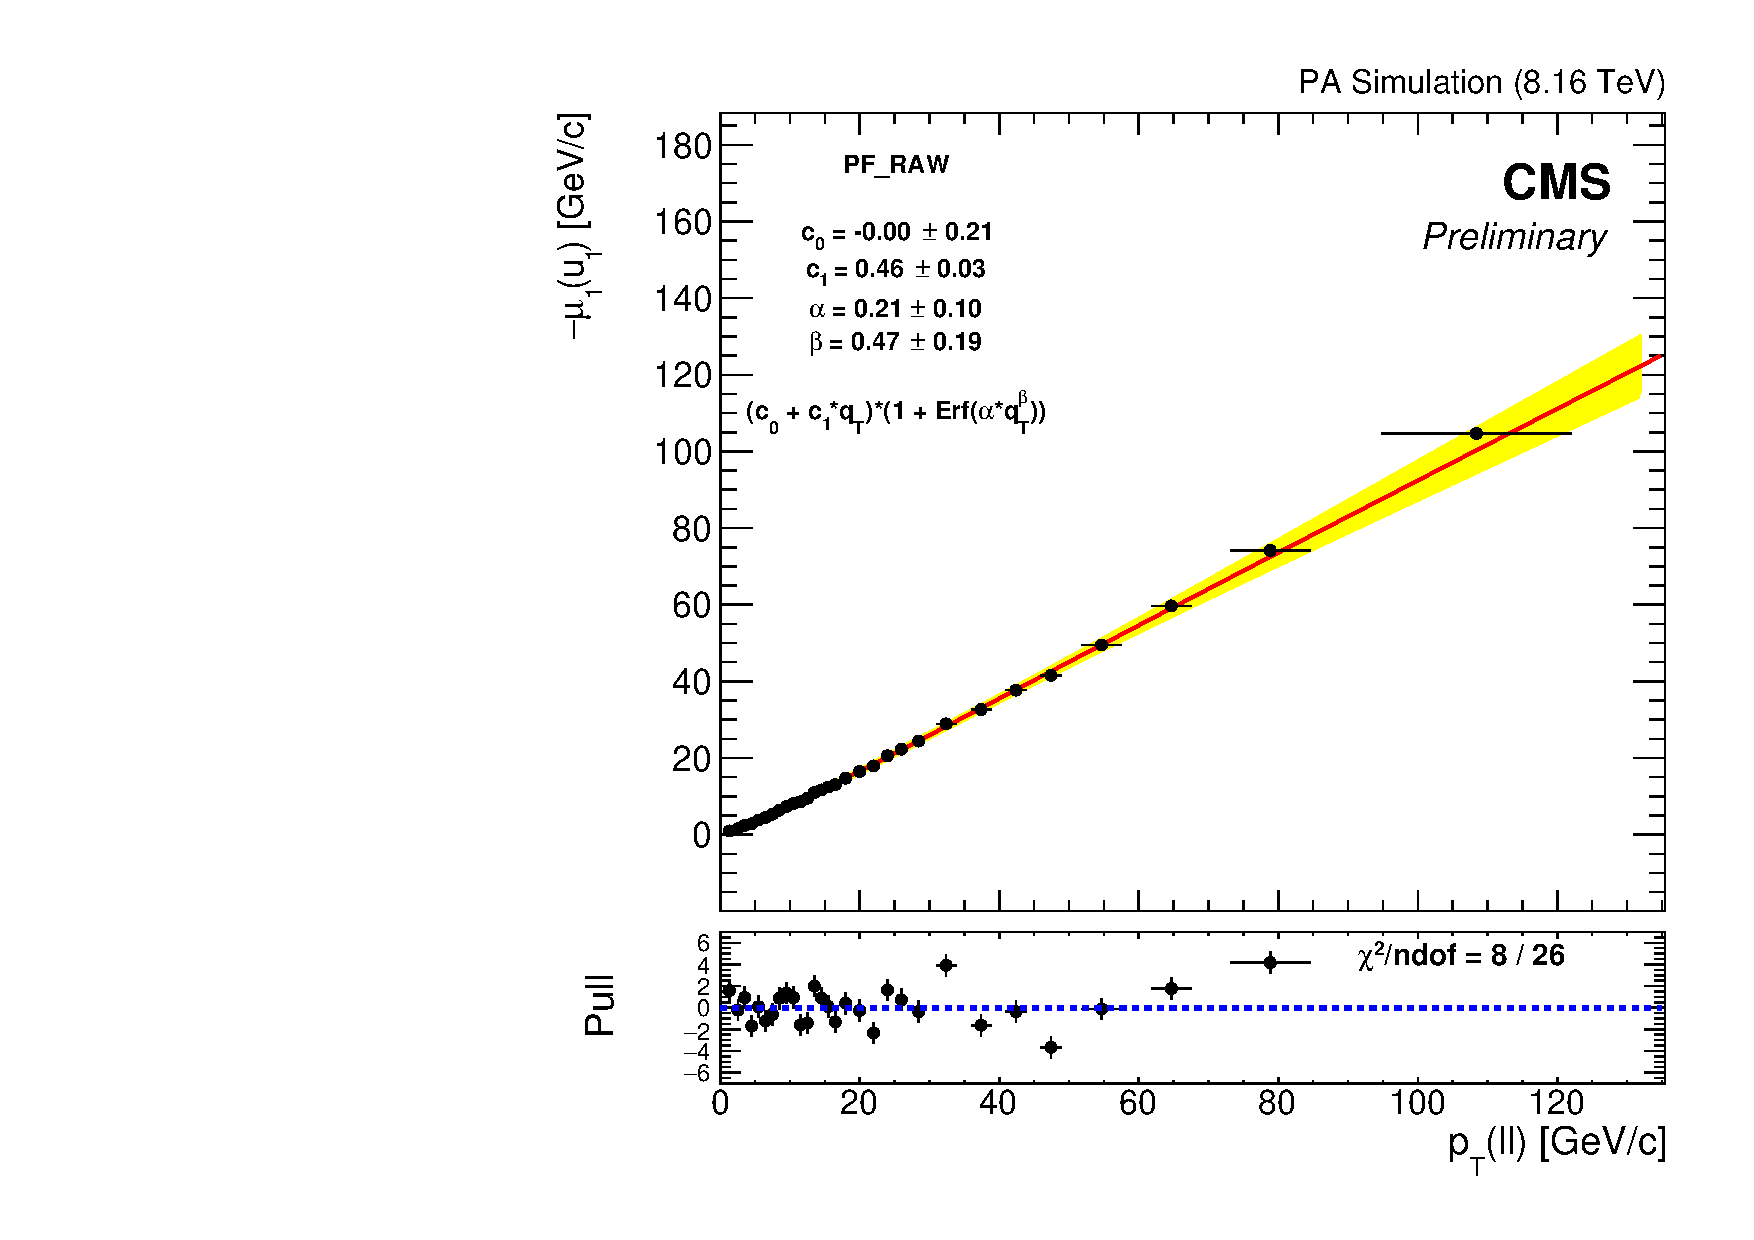
\includegraphics[width=0.3\textwidth]{Figures/WBoson/Analysis/Correction/Recoil/RecoilFitsqT/MC/fitPFu1mean1.pdf}
  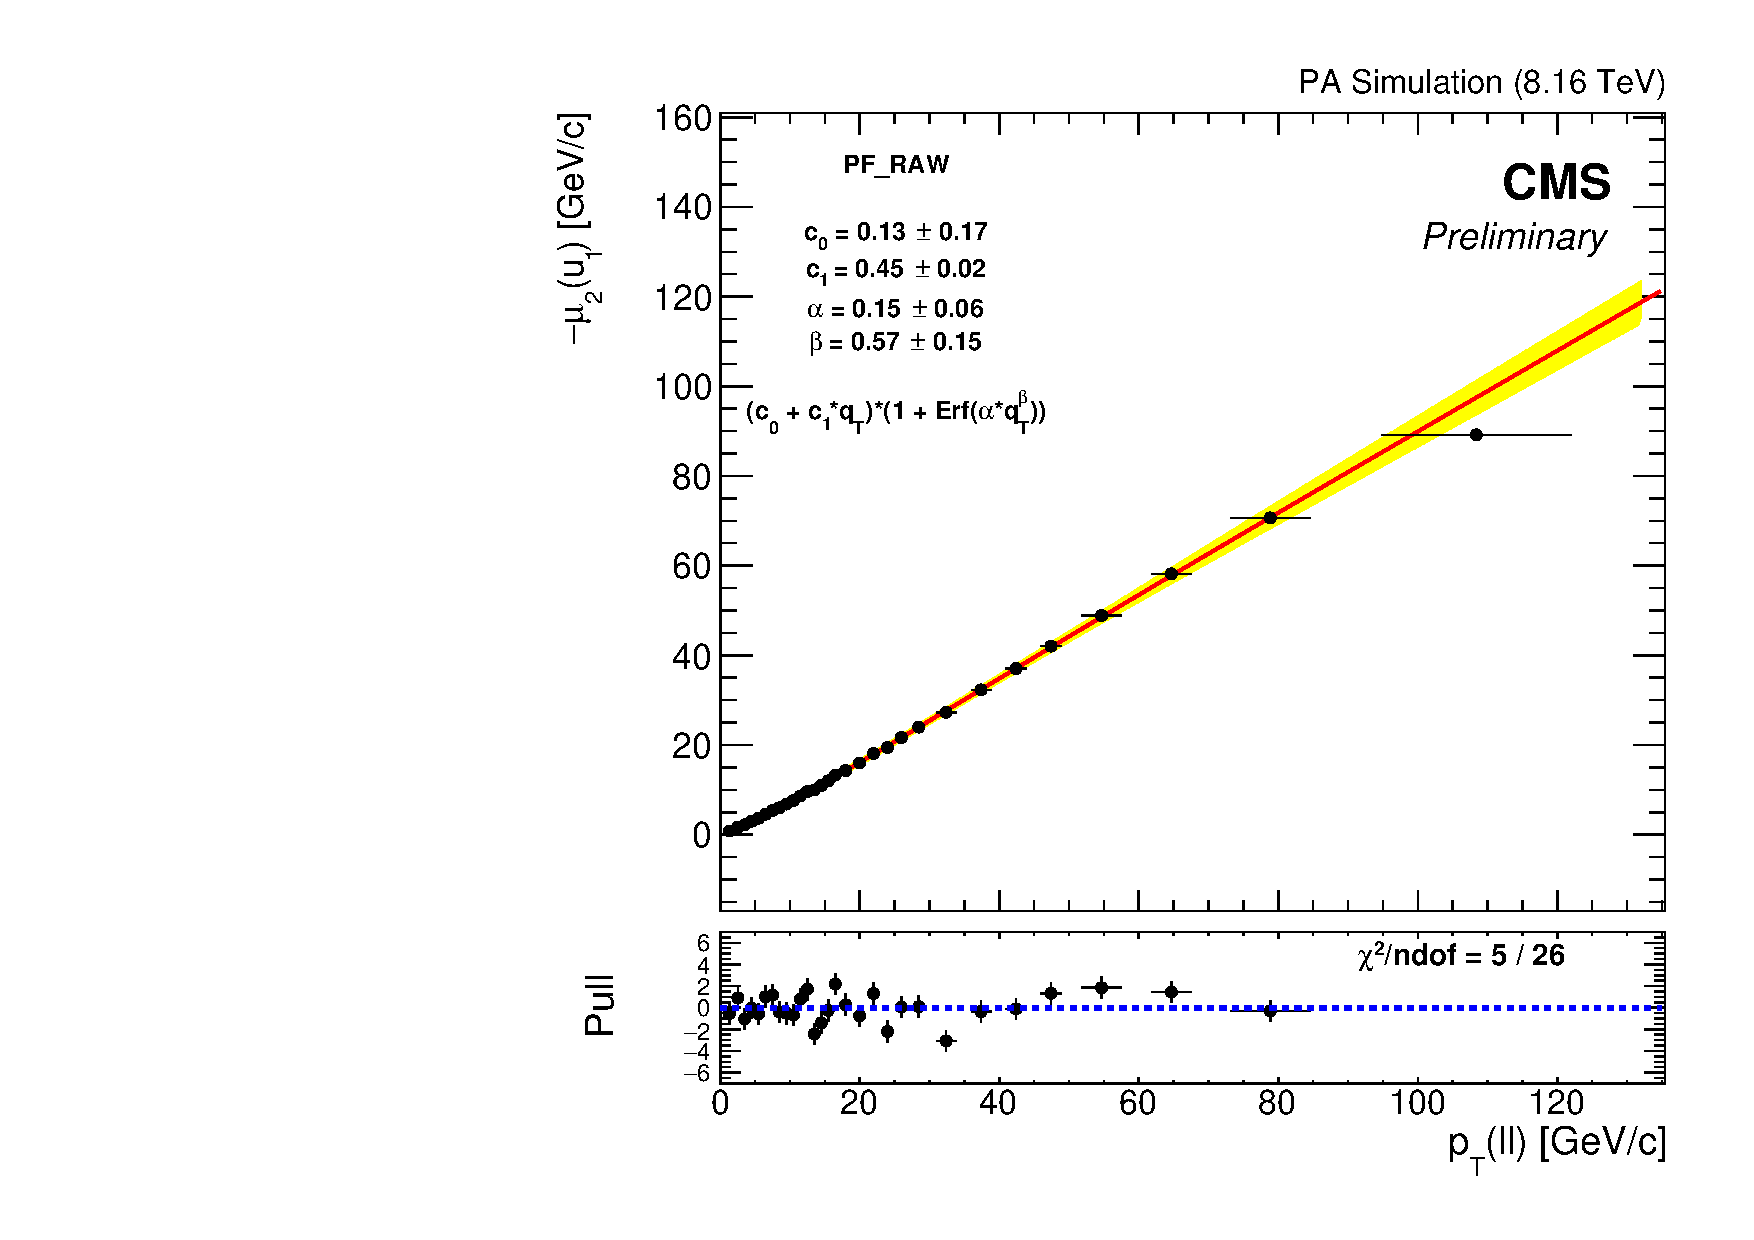
\includegraphics[width=0.3\textwidth]{Figures/WBoson/Analysis/Correction/Recoil/RecoilFitsqT/MC/fitPFu1mean2.pdf}
  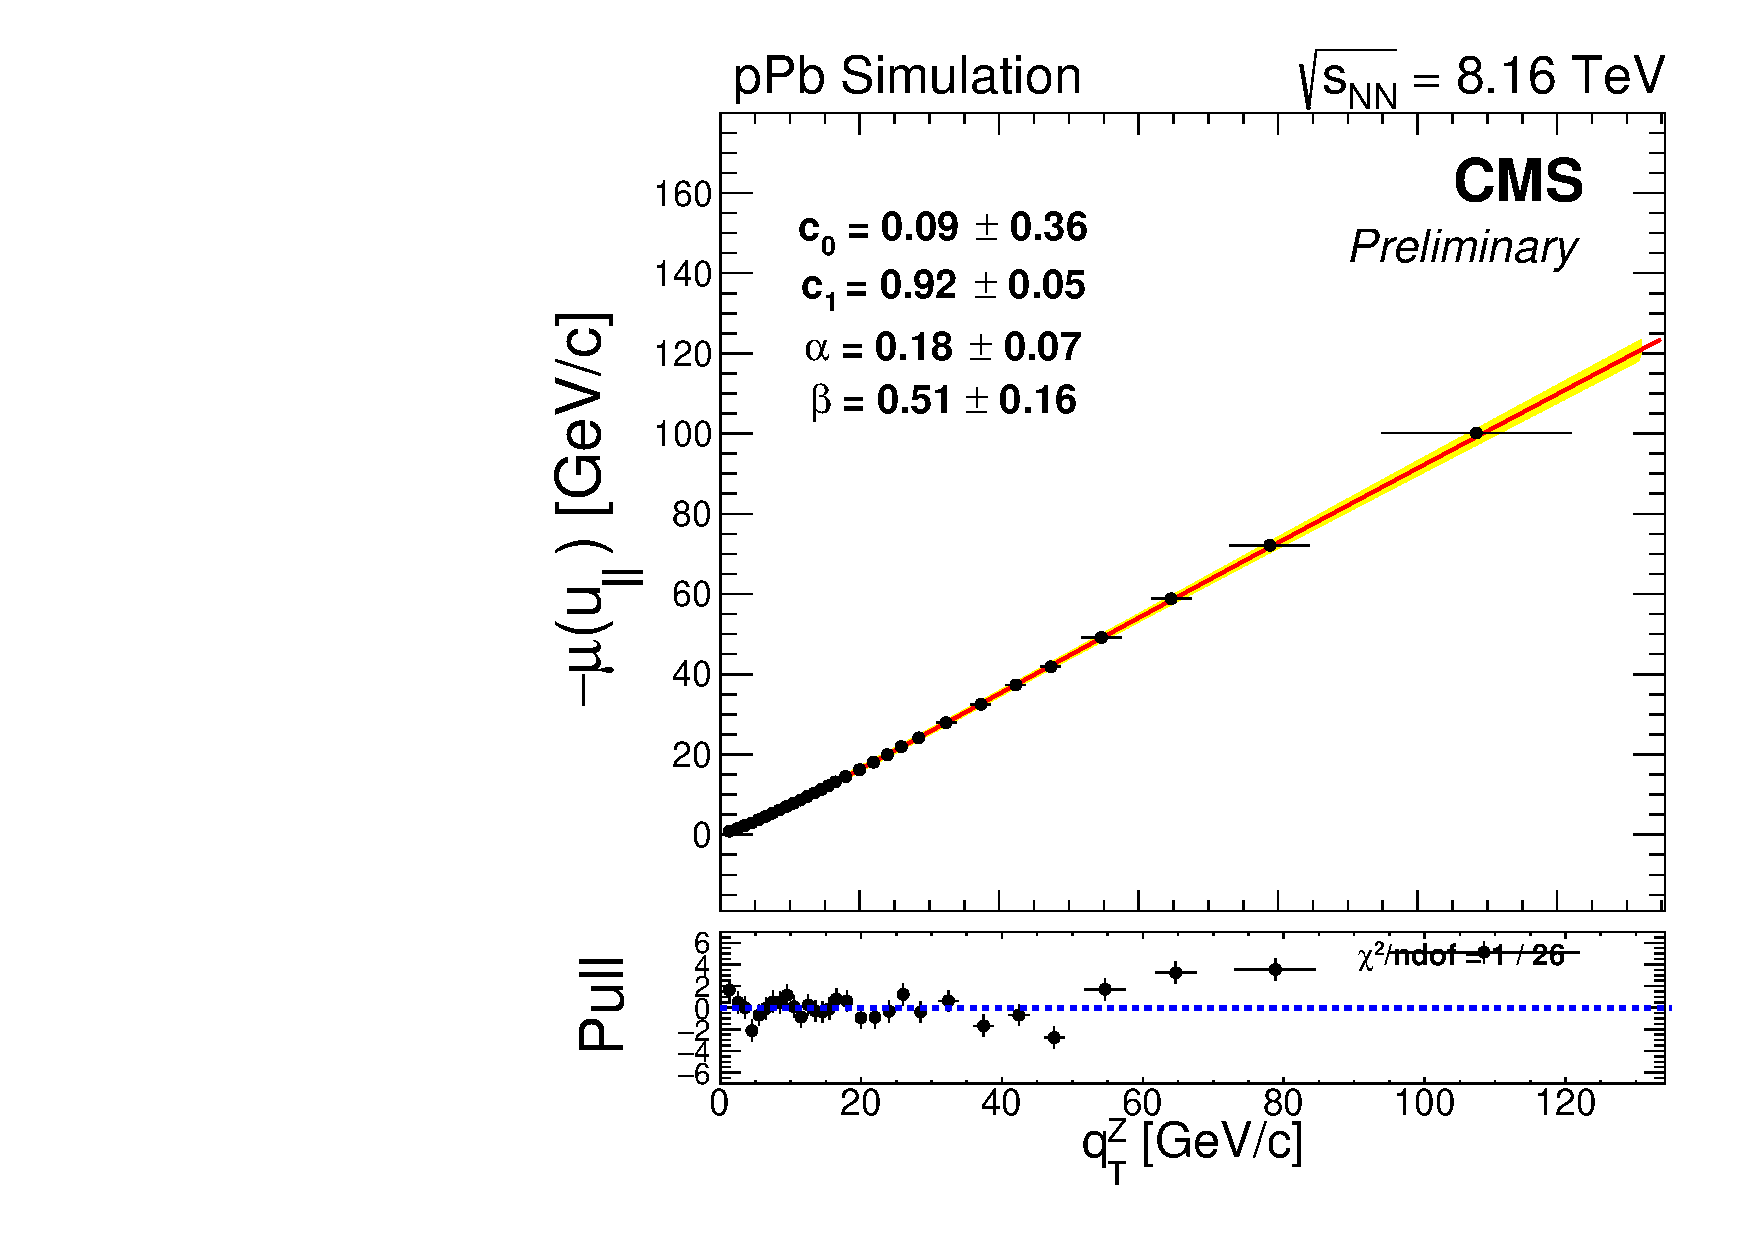
\includegraphics[width=0.3\textwidth]{Figures/WBoson/Analysis/Correction/Recoil/RecoilFitsqT/MC/fitPFu1mean.pdf}
 \caption{Fits for the $\mu_{1}$ (left), $\mu_{2}$ (middle) and weighted average $\mu$ (right) values of the parallel recoil component versus $q_{T}$. The plots on the top correspond to data while the plots in the bottom correspond to \ZToMuMu MC.}
 \label{fig:figU1RecoilScaleFit}
 \end{center}
\end{figure}

The average values of the perpendicular component of the recoil ($u_{2}$) from data and MC \Z samples are fitted with a constant function ($c_{0}$). The outcome is shown in \fig{fig:figU2RecoilScaleFit}. One observe that the average perpendicular component is consistent with zero, and so, it is set to zero in the correction procedure.

\begin{figure}
 \begin{center}
  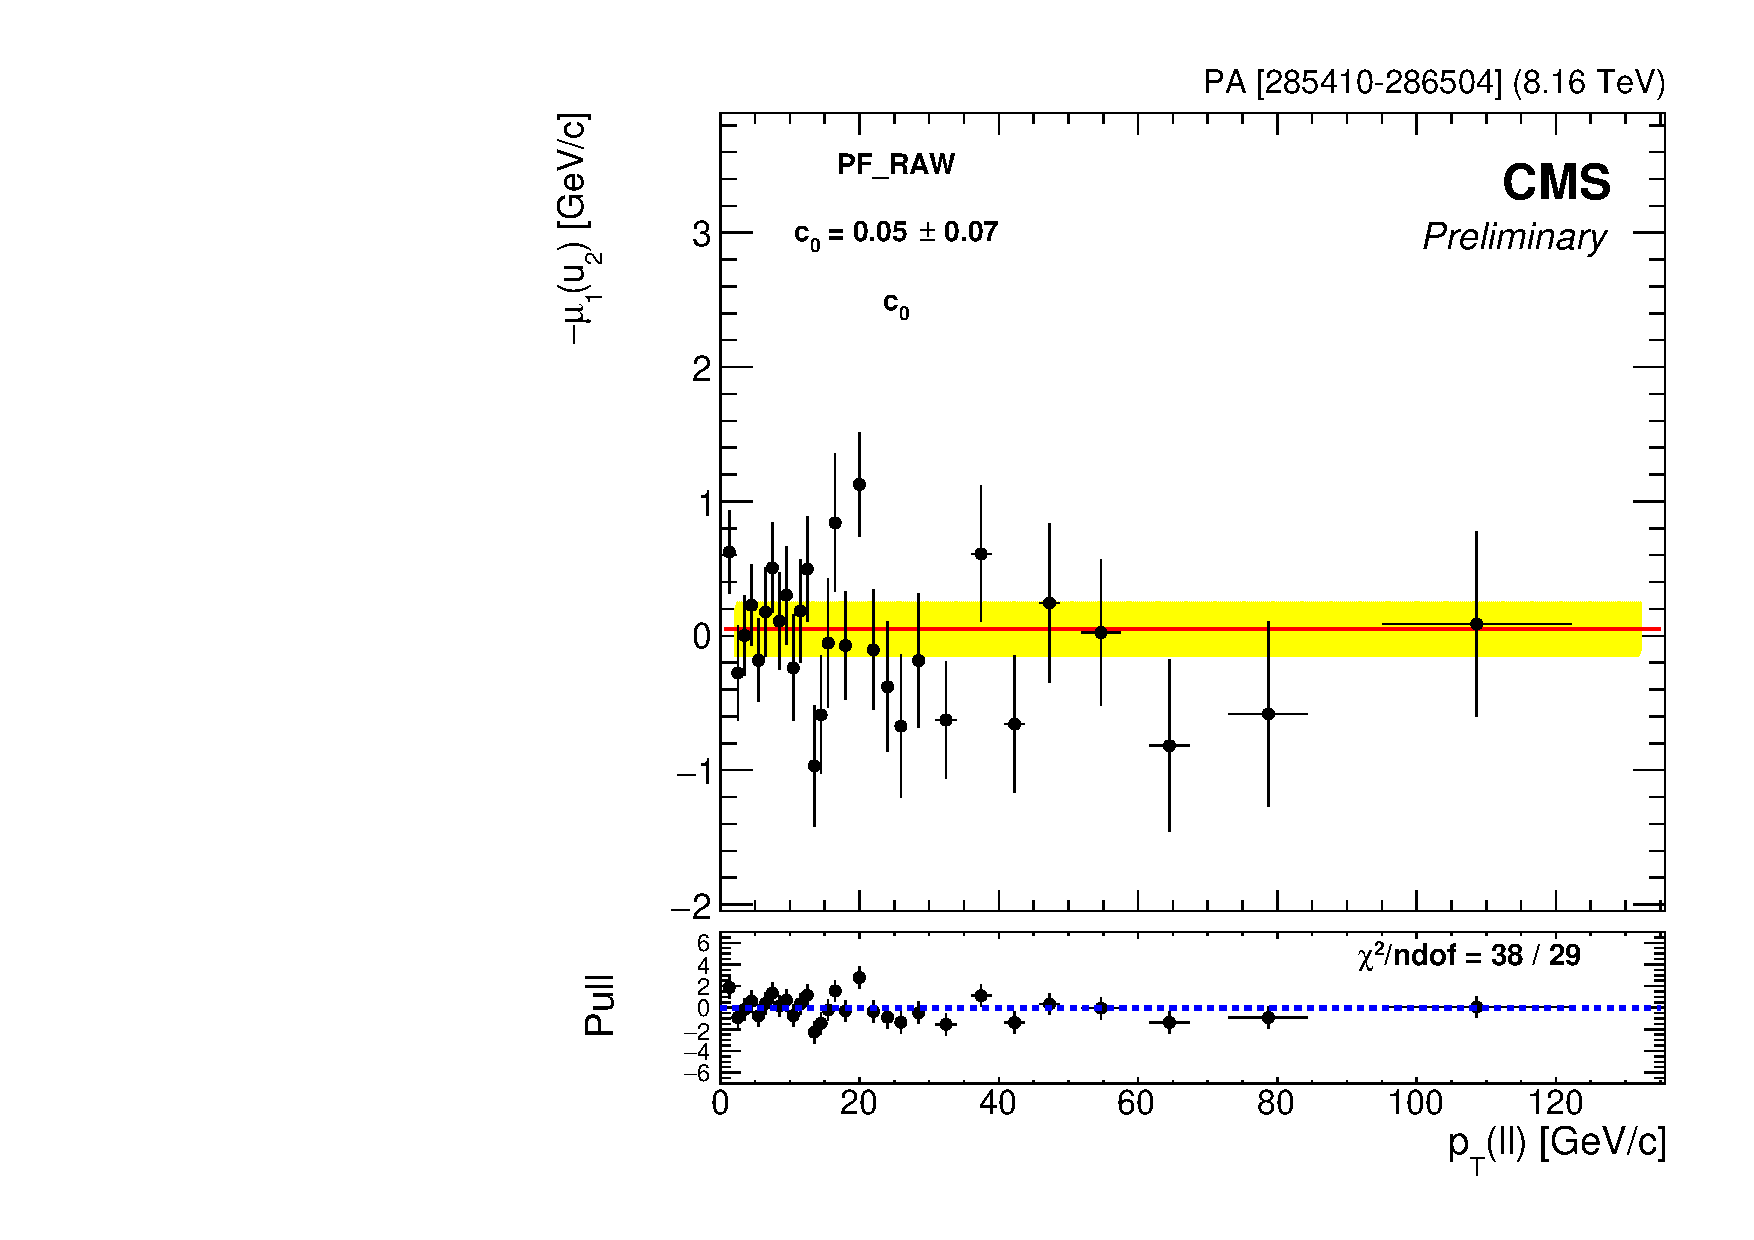
\includegraphics[width=0.3\textwidth]{Figures/WBoson/Analysis/Correction/Recoil/RecoilFitsqT/Data/fitPFu2mean1.pdf}
  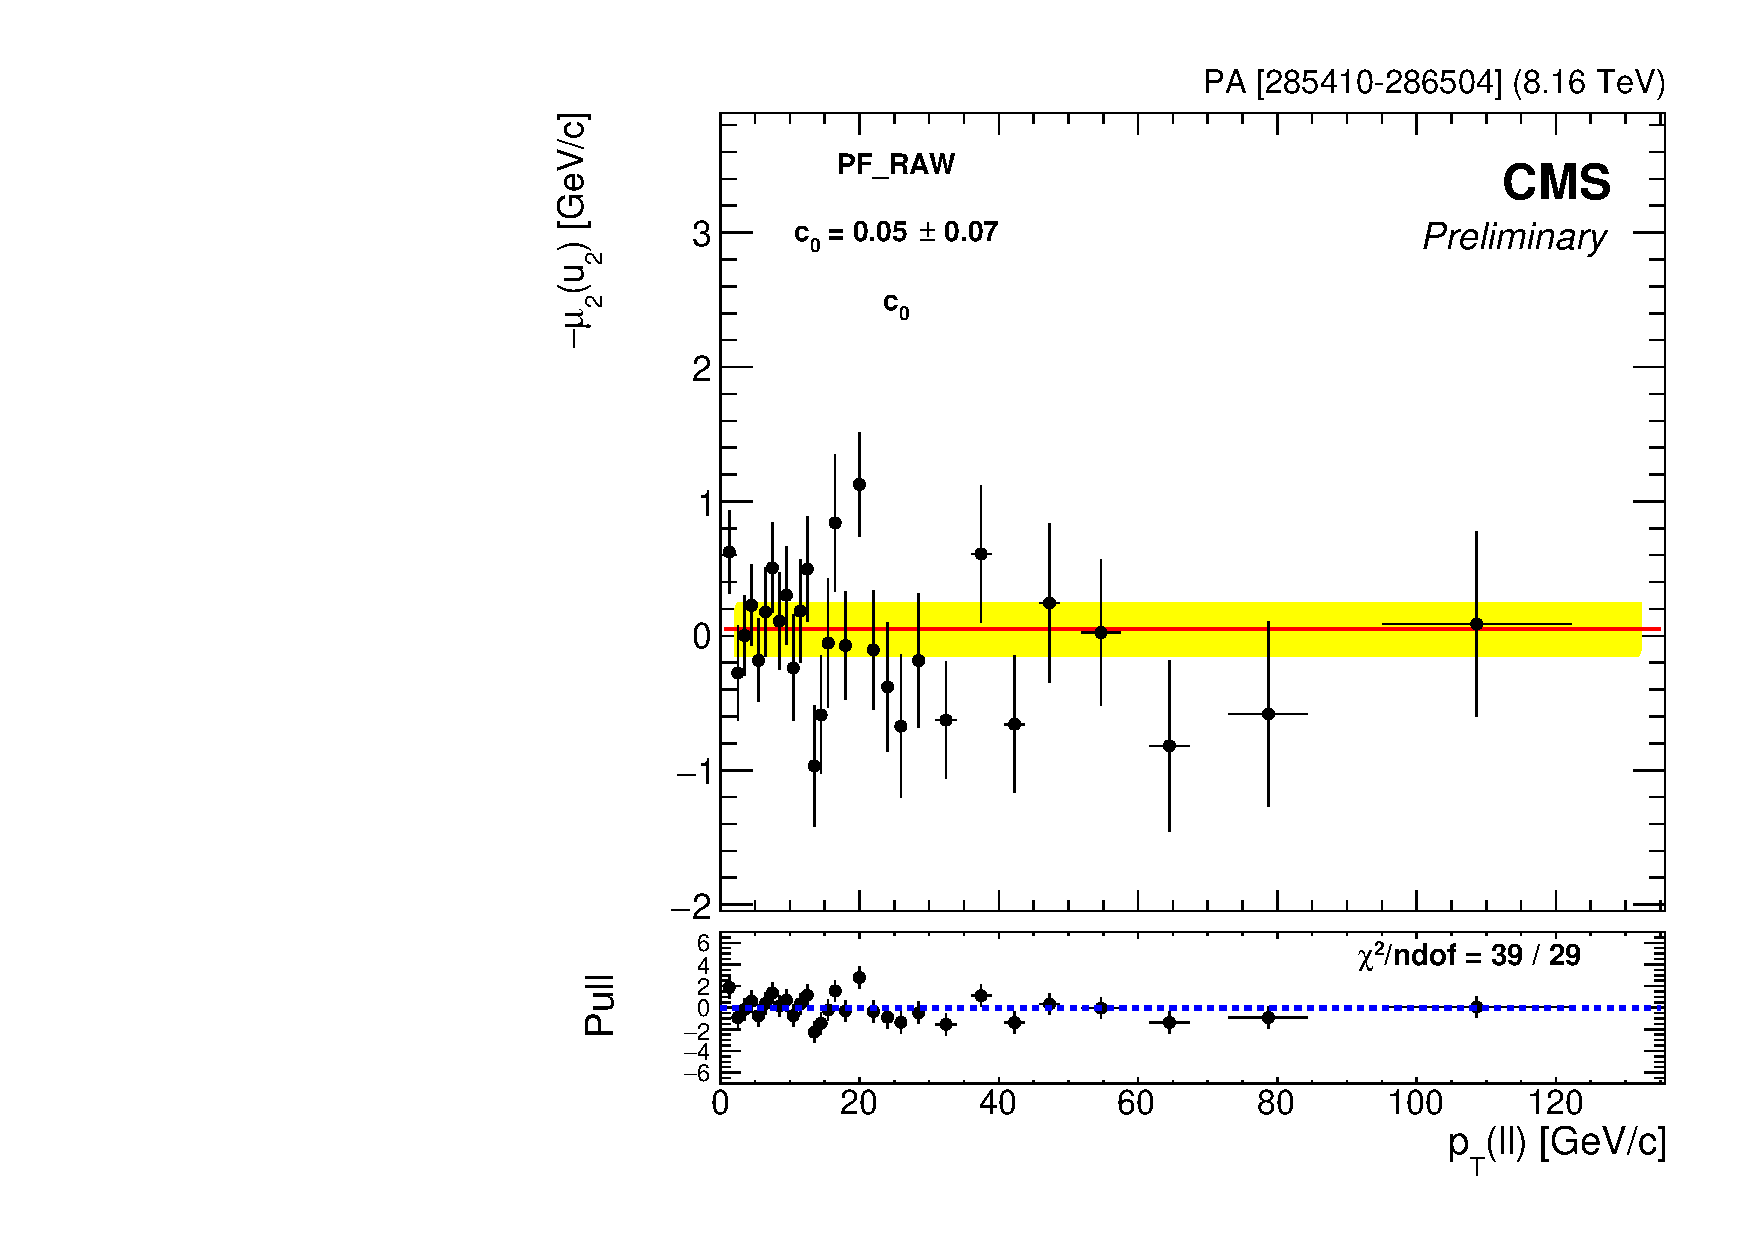
\includegraphics[width=0.3\textwidth]{Figures/WBoson/Analysis/Correction/Recoil/RecoilFitsqT/Data/fitPFu2mean2.pdf}
  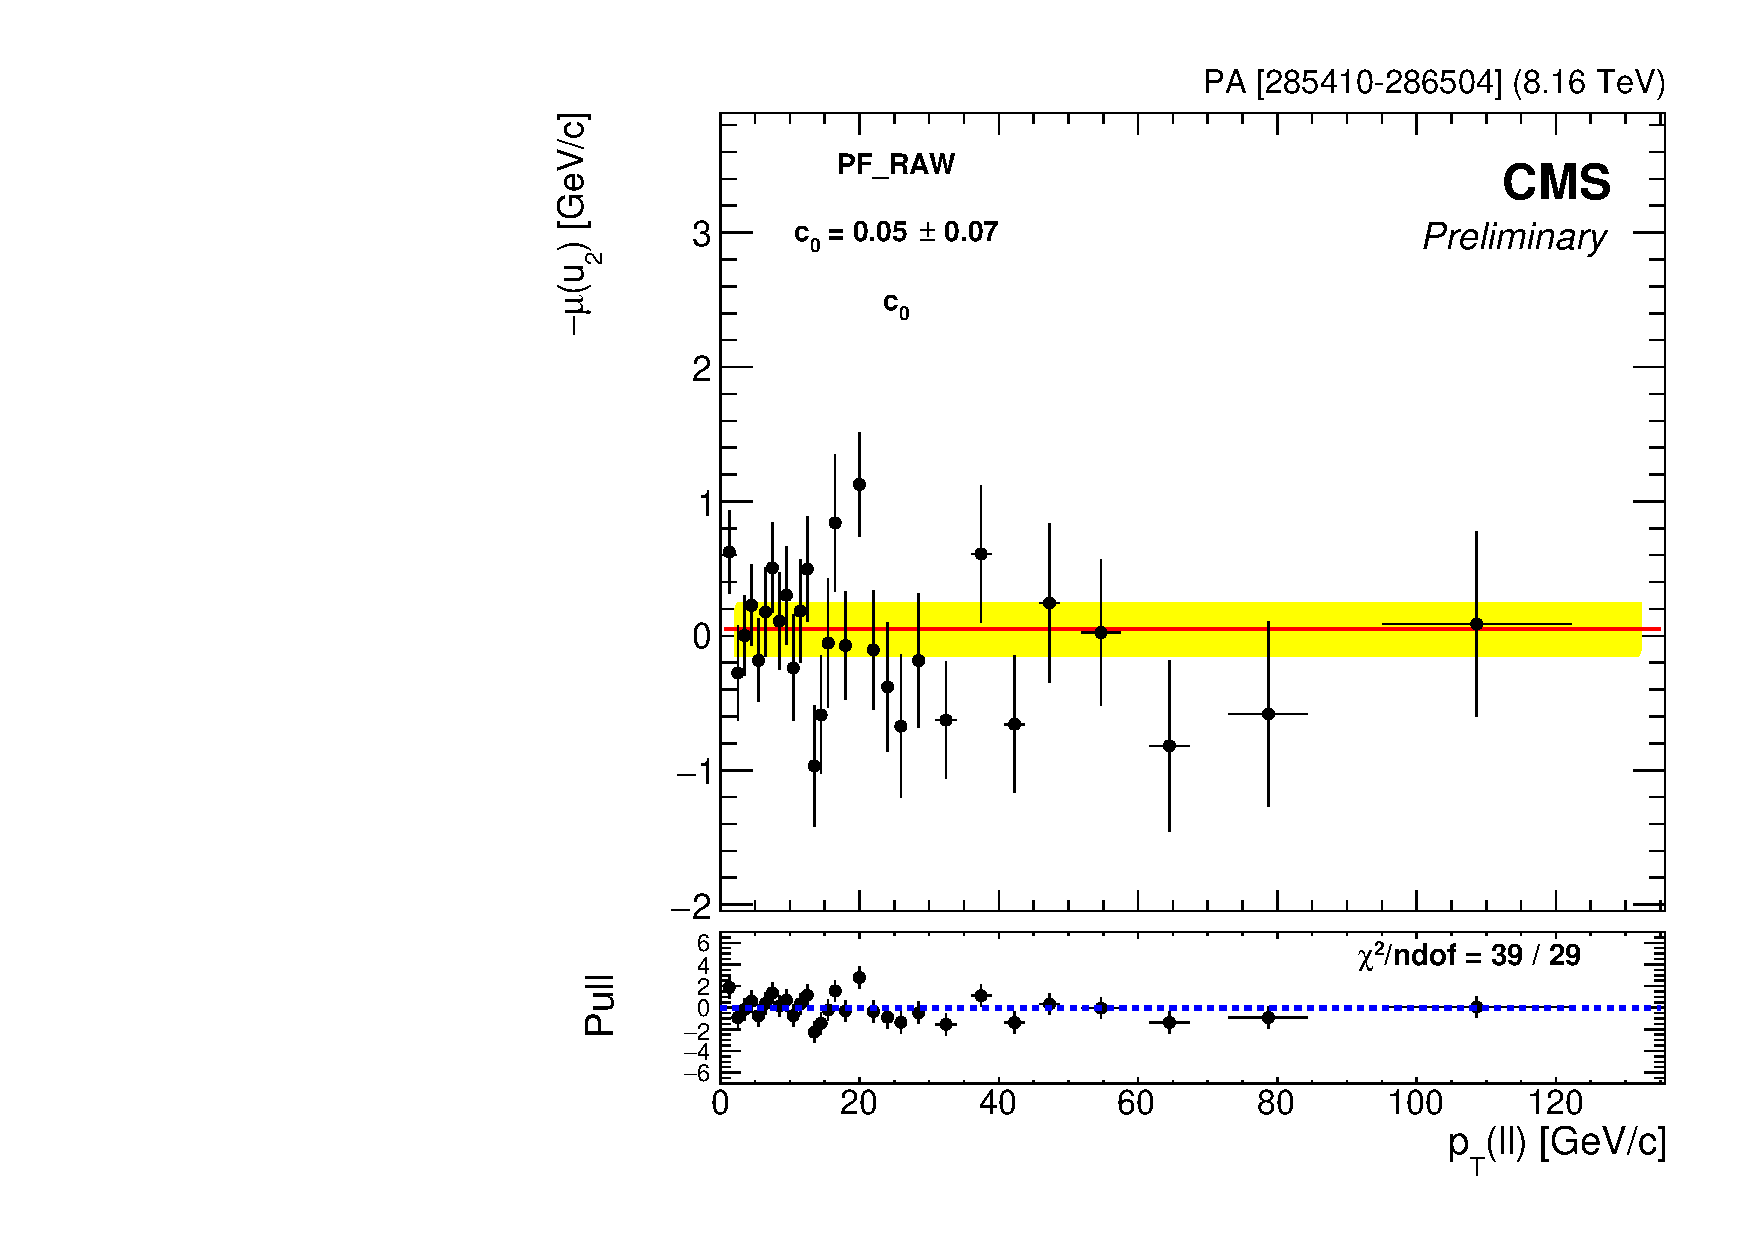
\includegraphics[width=0.3\textwidth]{Figures/WBoson/Analysis/Correction/Recoil/RecoilFitsqT/Data/fitPFu2mean.pdf} \\
  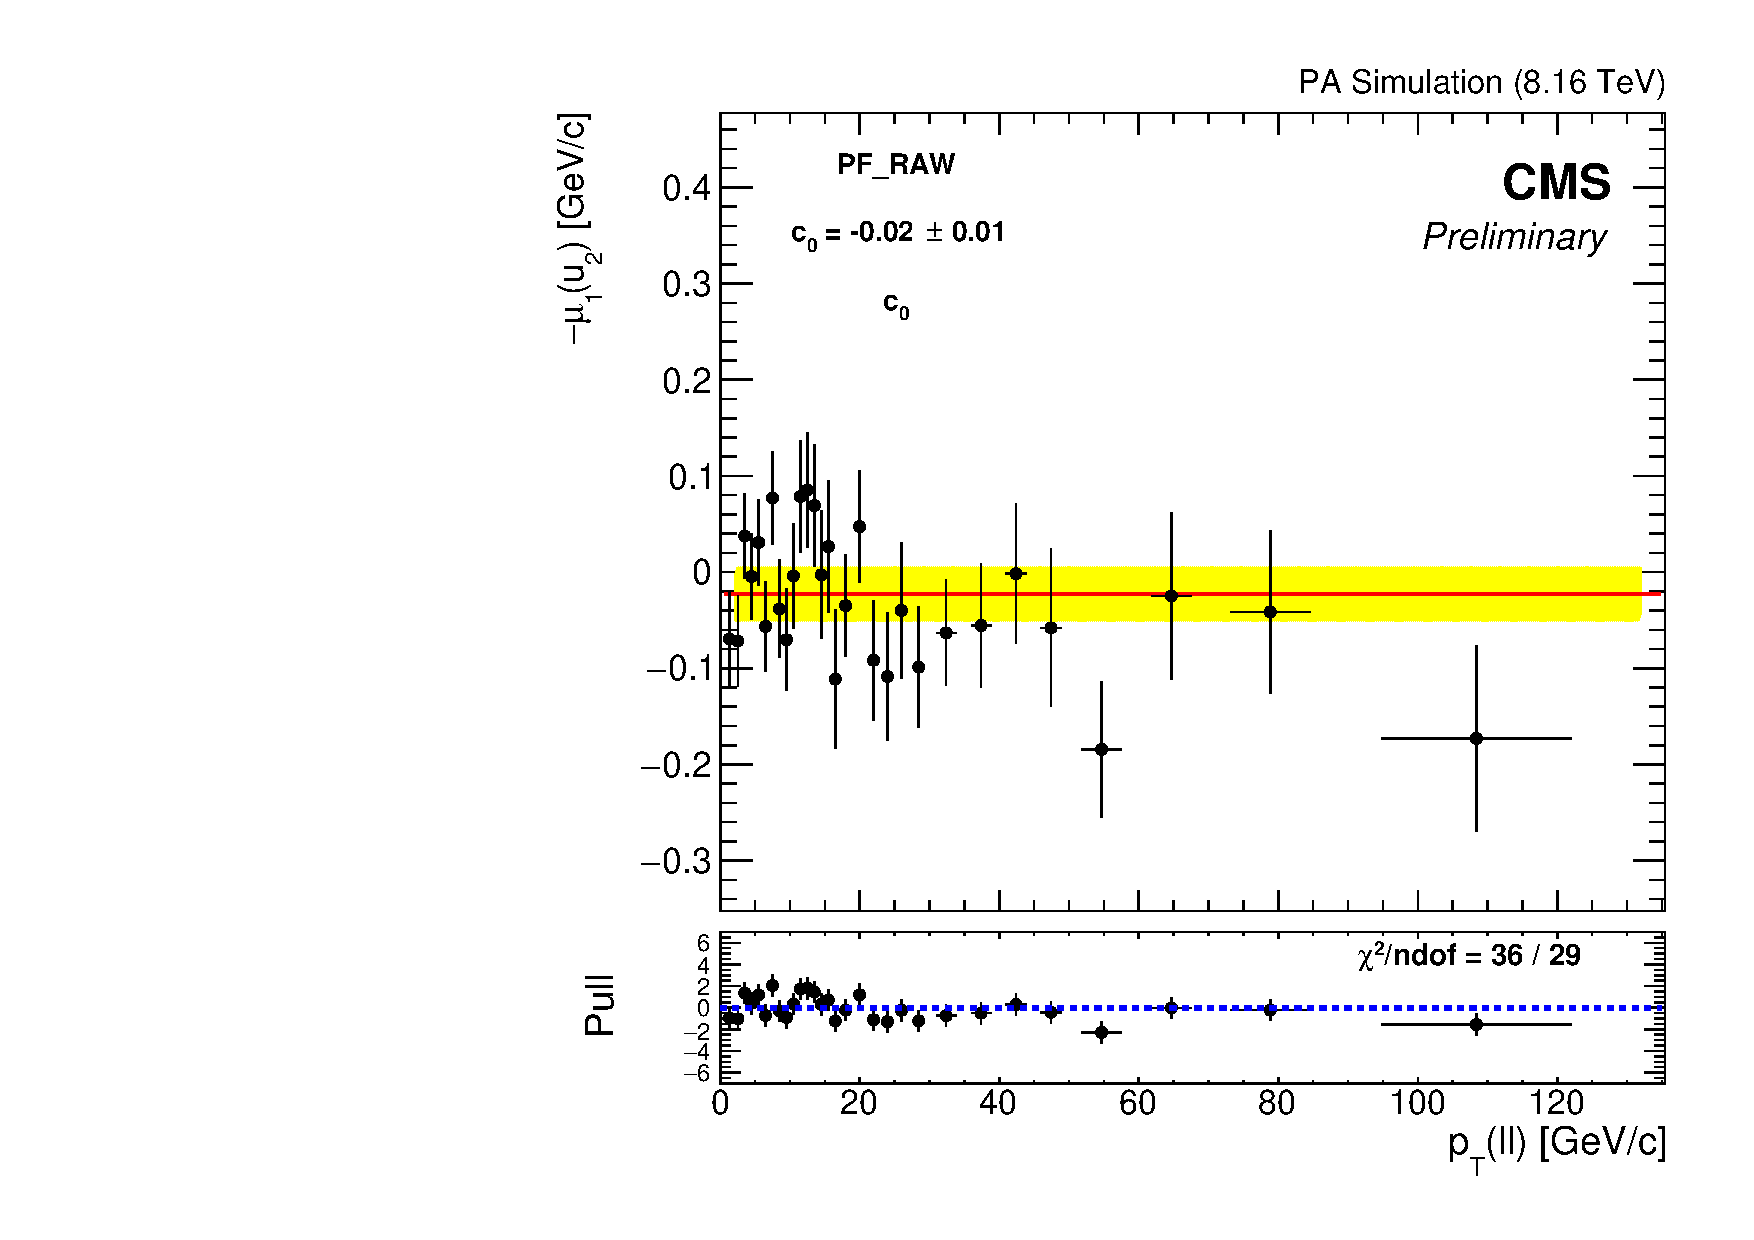
\includegraphics[width=0.3\textwidth]{Figures/WBoson/Analysis/Correction/Recoil/RecoilFitsqT/MC/fitPFu2mean1.pdf}
  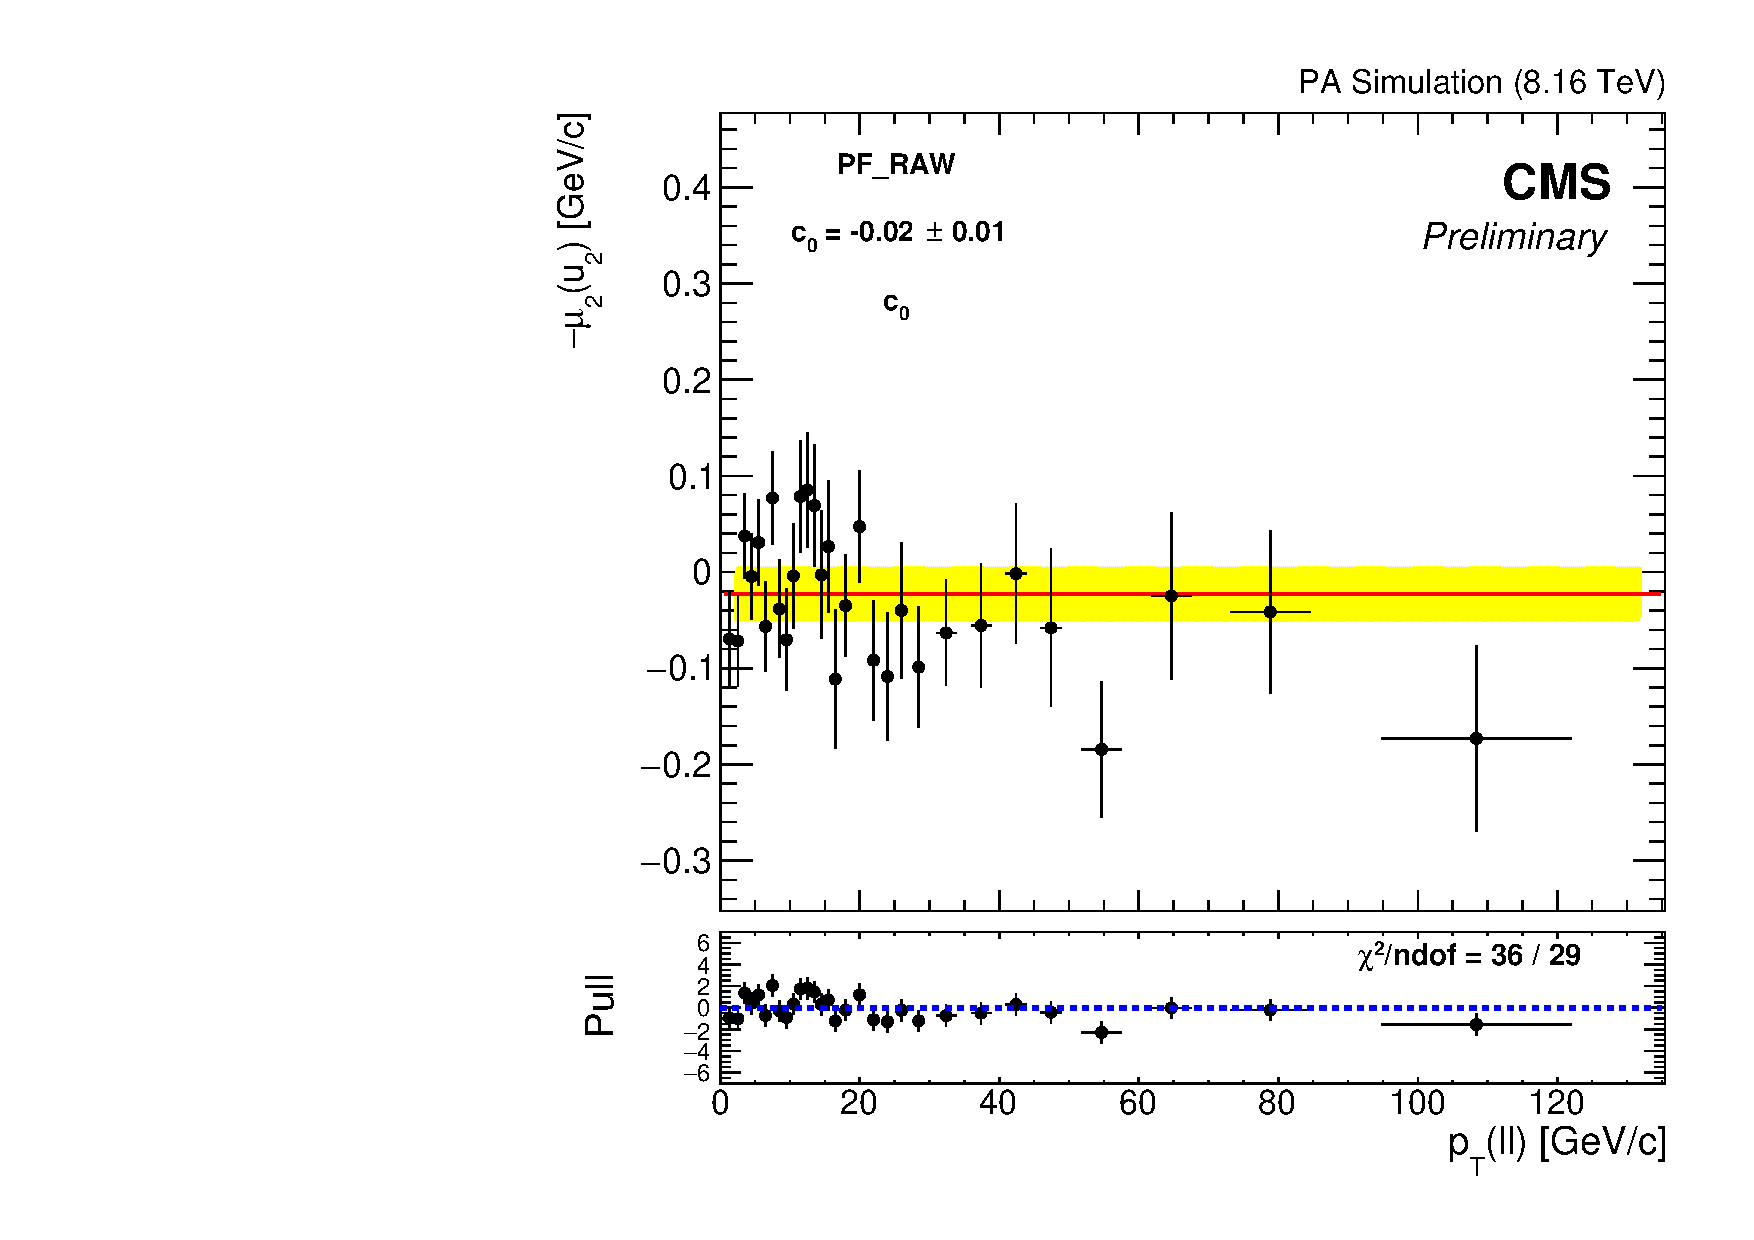
\includegraphics[width=0.3\textwidth]{Figures/WBoson/Analysis/Correction/Recoil/RecoilFitsqT/MC/fitPFu2mean2.pdf}
  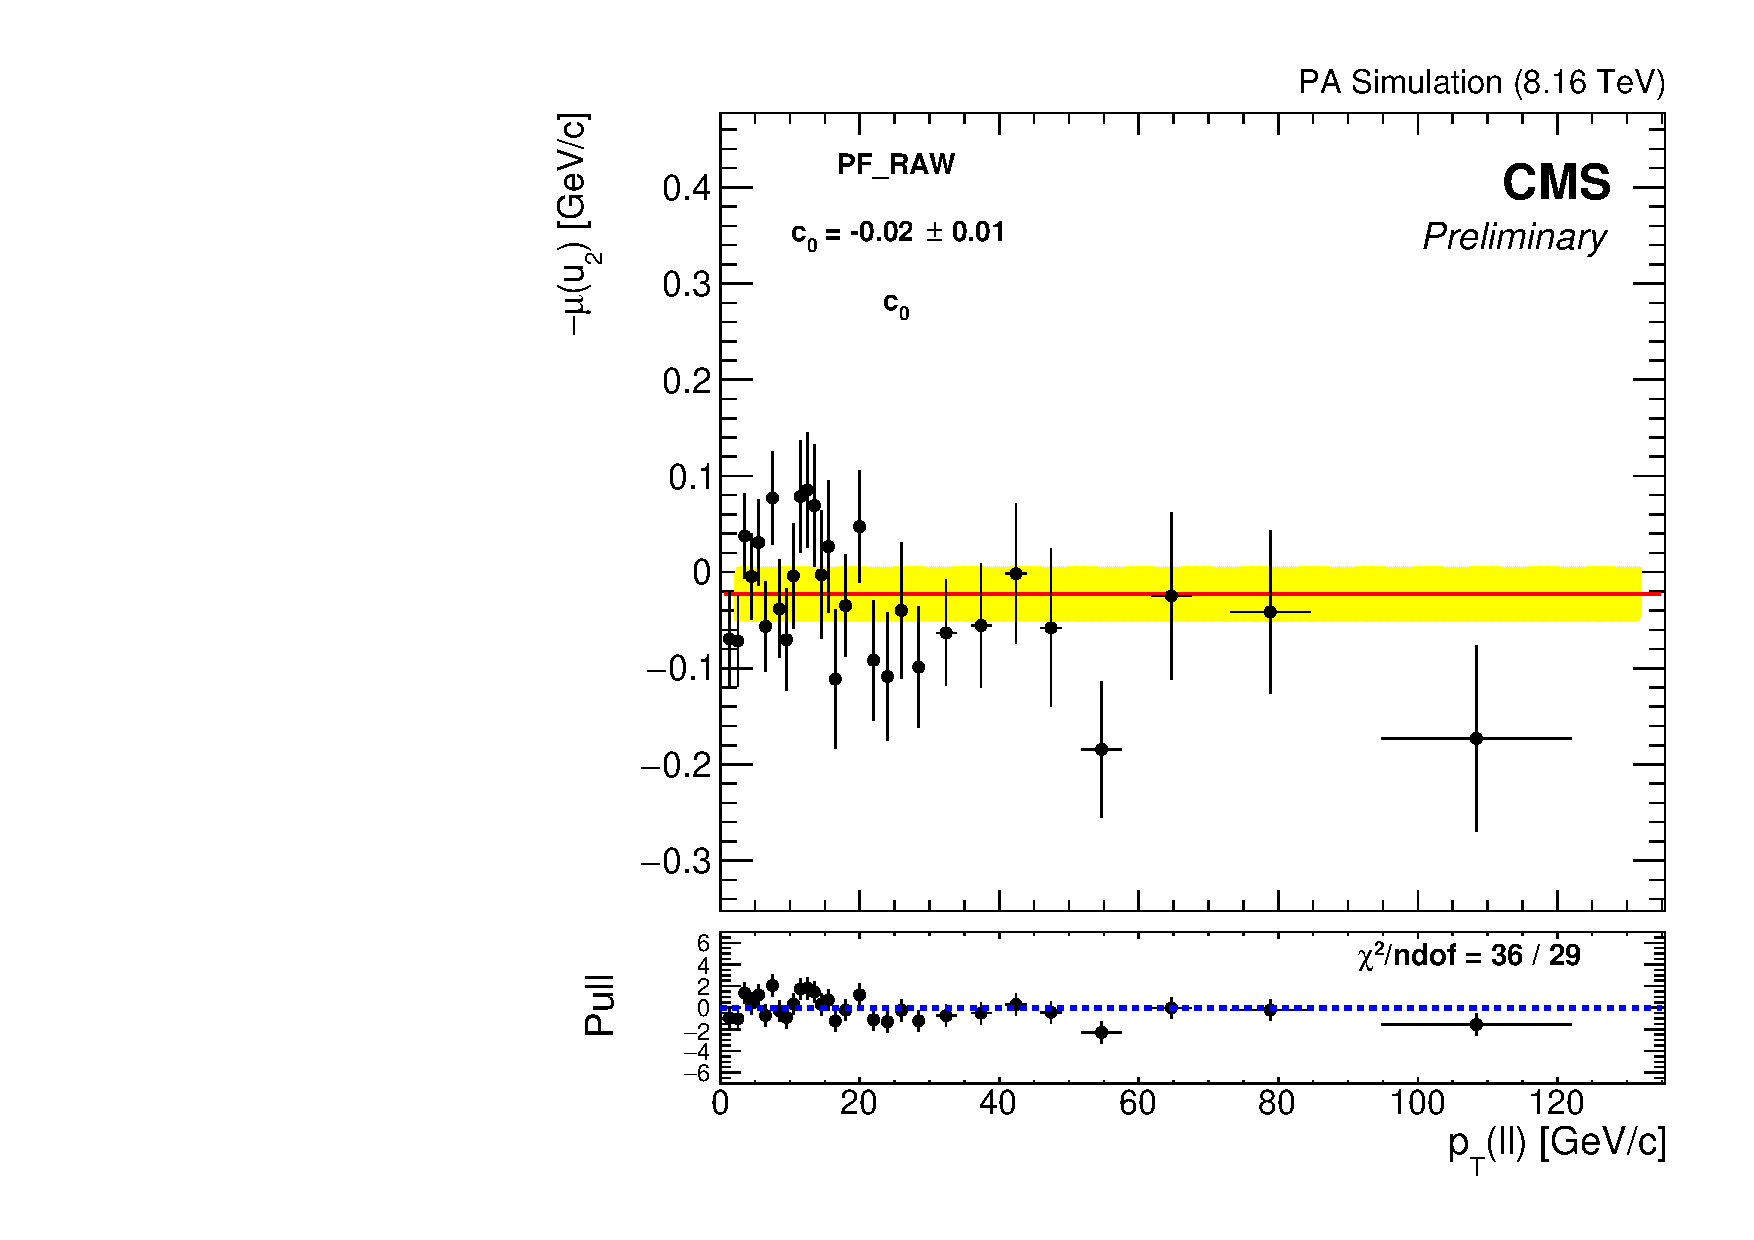
\includegraphics[width=0.3\textwidth]{Figures/WBoson/Analysis/Correction/Recoil/RecoilFitsqT/MC/fitPFu2mean.pdf}
 \caption{Fits for the $\mu_{1}$ (left), $\mu_{2}$ (middle) and weighted average $\mu$ (right) values of the perpendicular recoil component versus $q_{T}$. The plots on the top correspond to data while the plots in the bottom correspond to \ZToMuMu MC.}
 \label{fig:figU2RecoilScaleFit}
 \end{center}
\end{figure}


\subsubsection{Recoil Resolution}\label{sec:WBoson_Corrections_MET_Rres}

The gaussian widths ($\sigma_{1}$ and $\sigma_{2}$) of the parallel and perpendicular distributions of the recoil are also extracted from the recoil fits for each $q_{T}$ bin. The recoil resolution is   parametrised as a function of $q_{T}$ using the following formula:

\begin{equation}\label{eq:equreolnparam} 
\sigma_{1,2}(q_{T}) = \sqrt{s_{0}^{2} + s_{1}^{2} \cdot q_{T}^{\alpha}},
\end{equation}

The fits to the resolution profile of the parallel and perpendicular components of the recoil are presented in \fig{fig:figU1RecoilResolutionFit} and  \fig{fig:figU2RecoilResolutionFit}, respectively. Moreover, the distribution of the weighted average of the two gaussian widths, $\sigma = f \cdot \sigma_{1} + (1 - f) \cdot \sigma_{2}$, is also shown.

\begin{figure} [h!]
 \begin{center}
  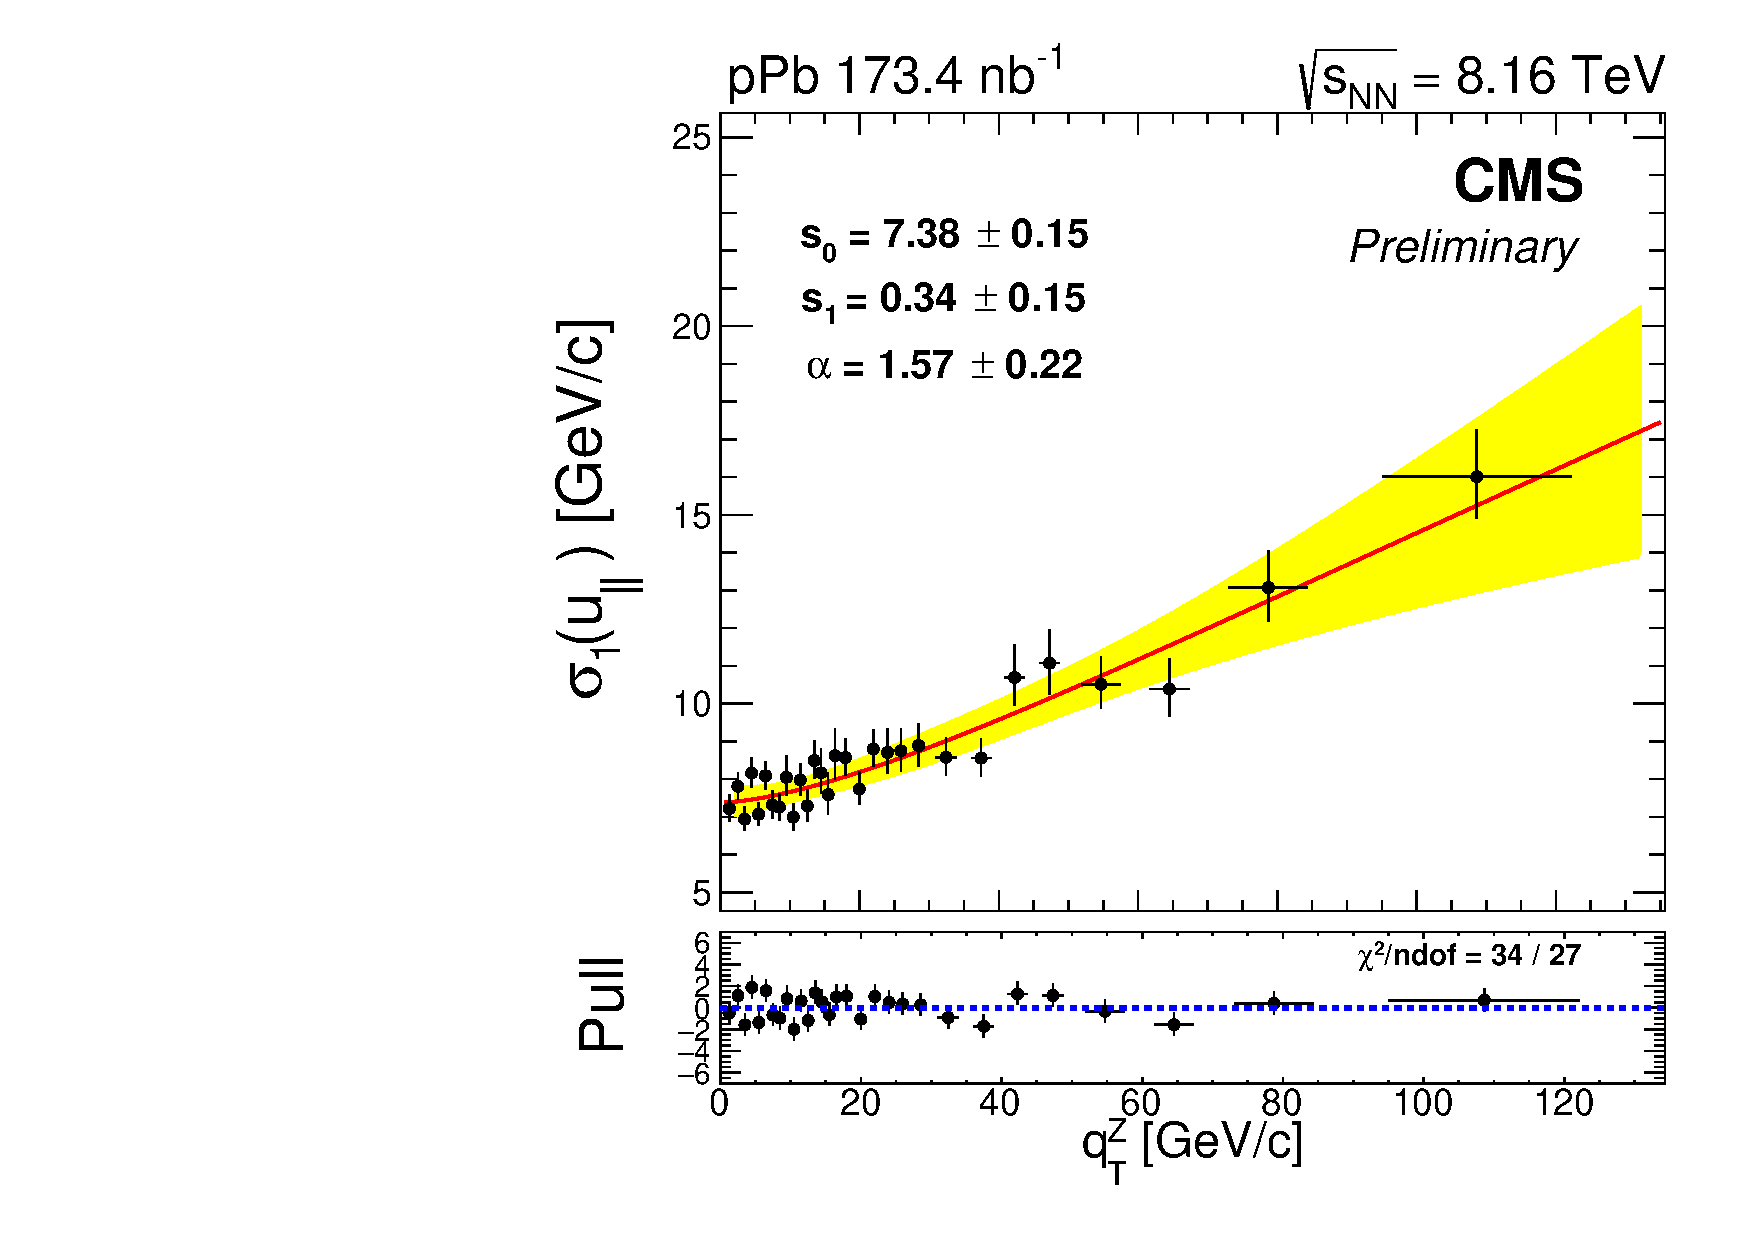
\includegraphics[width=0.3\textwidth]{Figures/WBoson/Analysis/Correction/Recoil/RecoilFitsqT/Data/fitPFu1sigma1.pdf}
  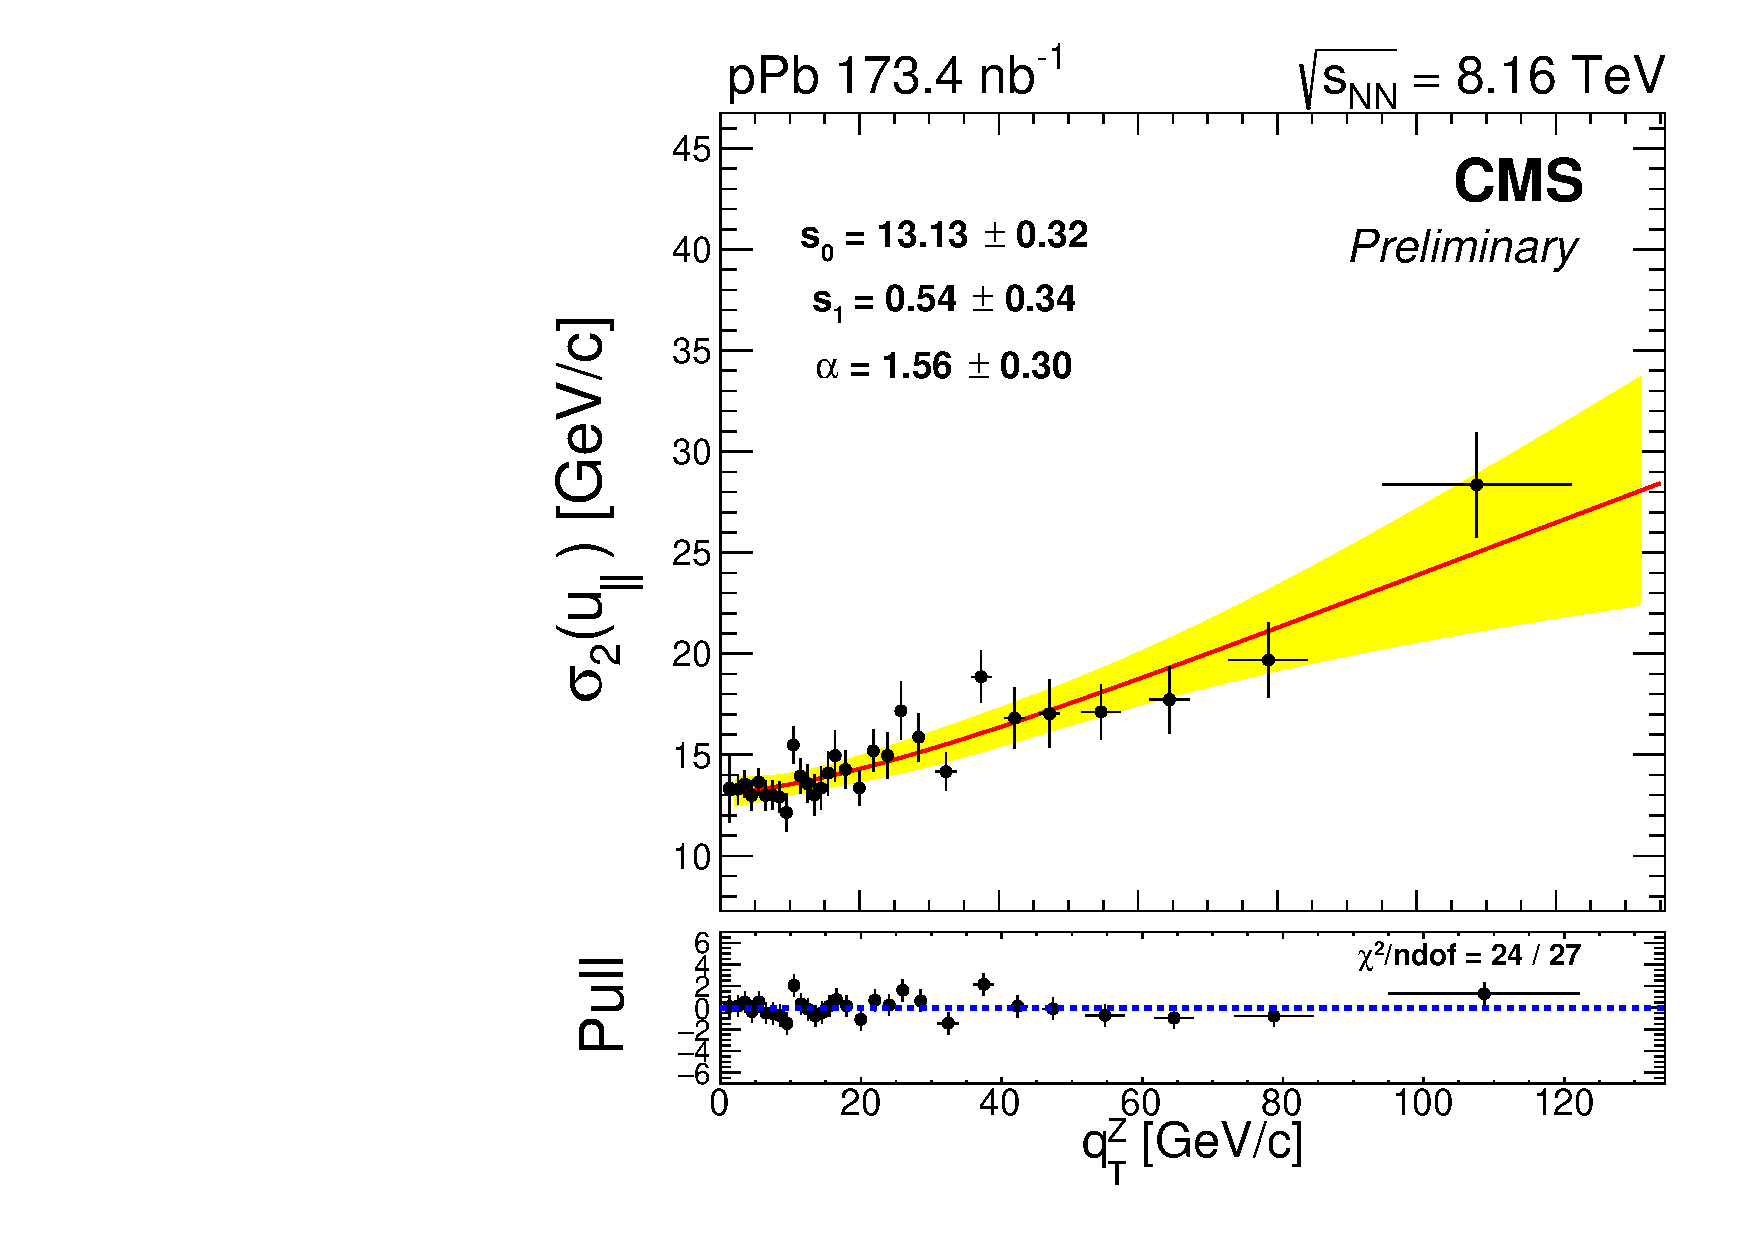
\includegraphics[width=0.3\textwidth]{Figures/WBoson/Analysis/Correction/Recoil/RecoilFitsqT/Data/fitPFu1sigma2.pdf}
  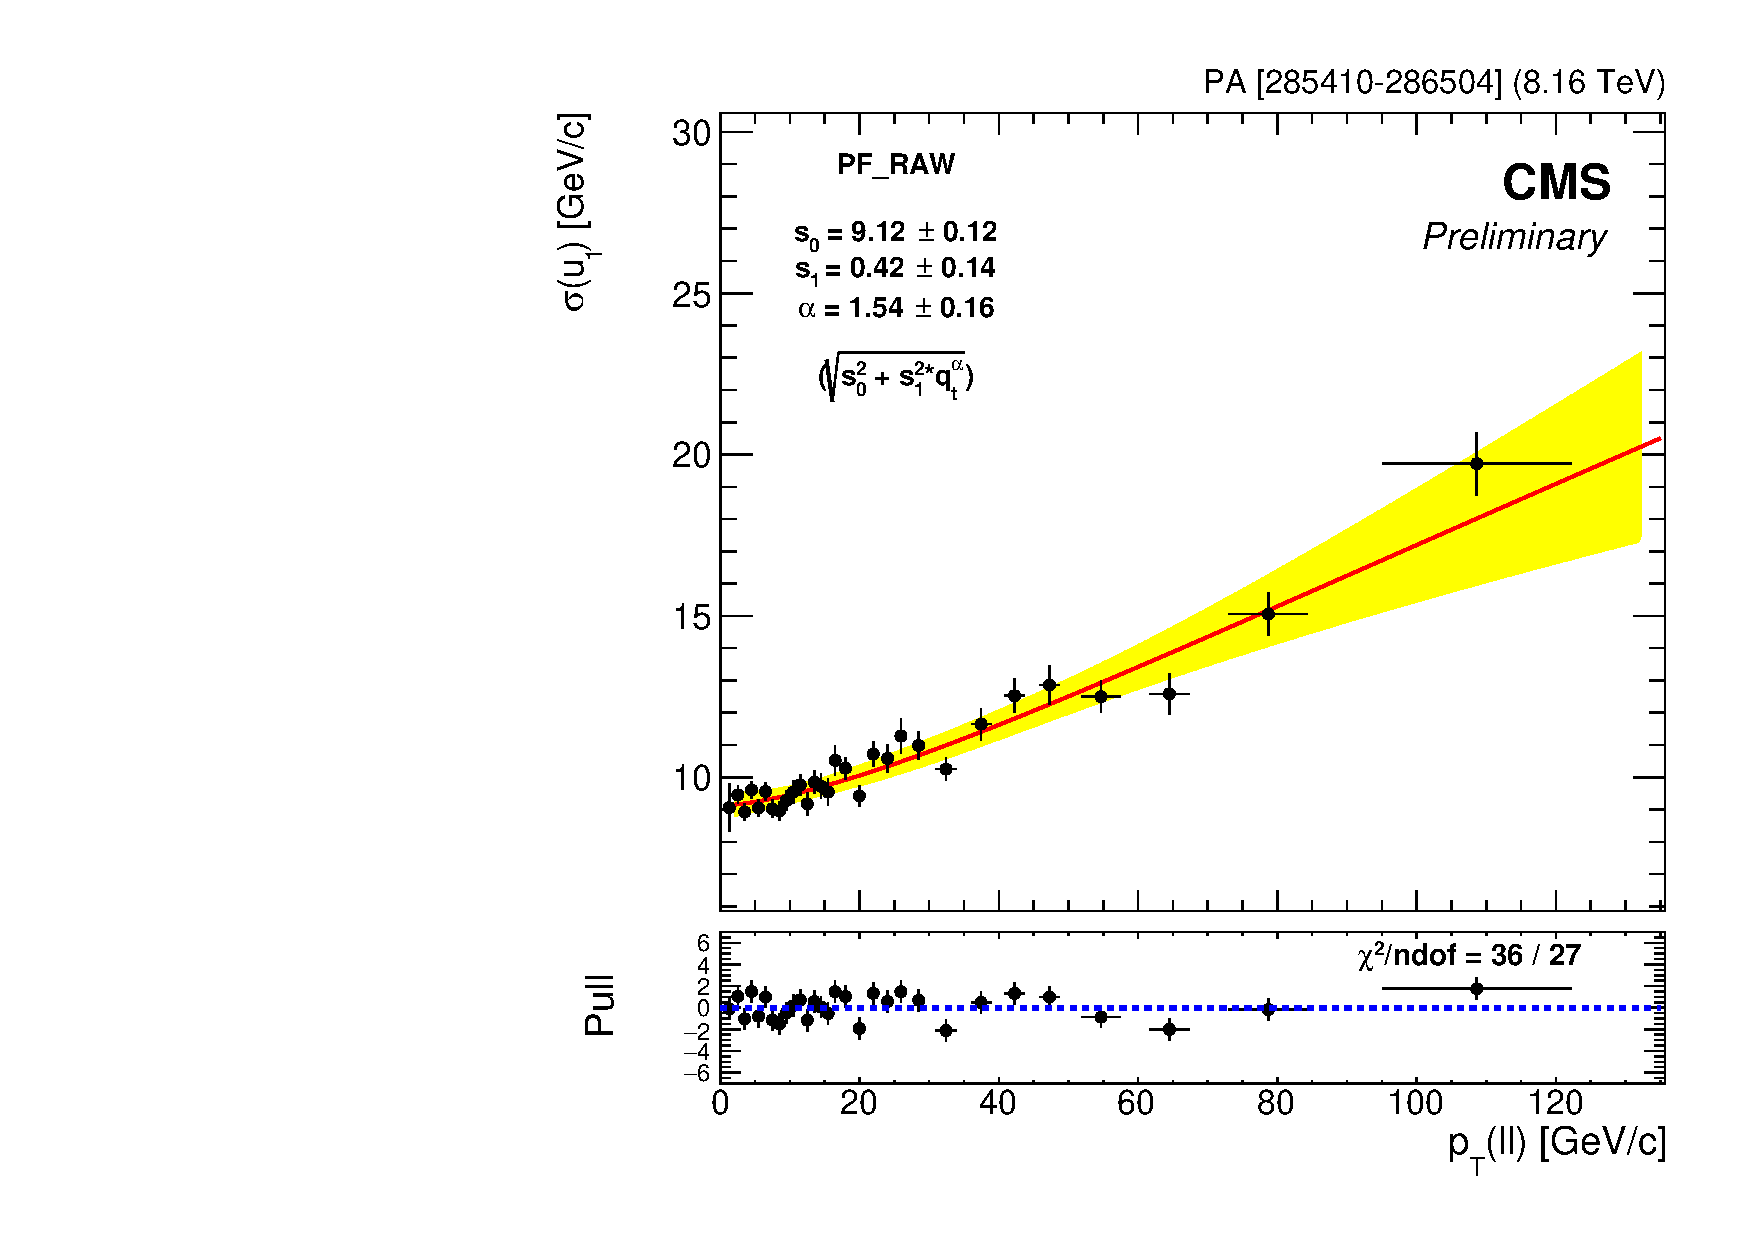
\includegraphics[width=0.3\textwidth]{Figures/WBoson/Analysis/Correction/Recoil/RecoilFitsqT/Data/fitPFu1sigma.pdf} \\
  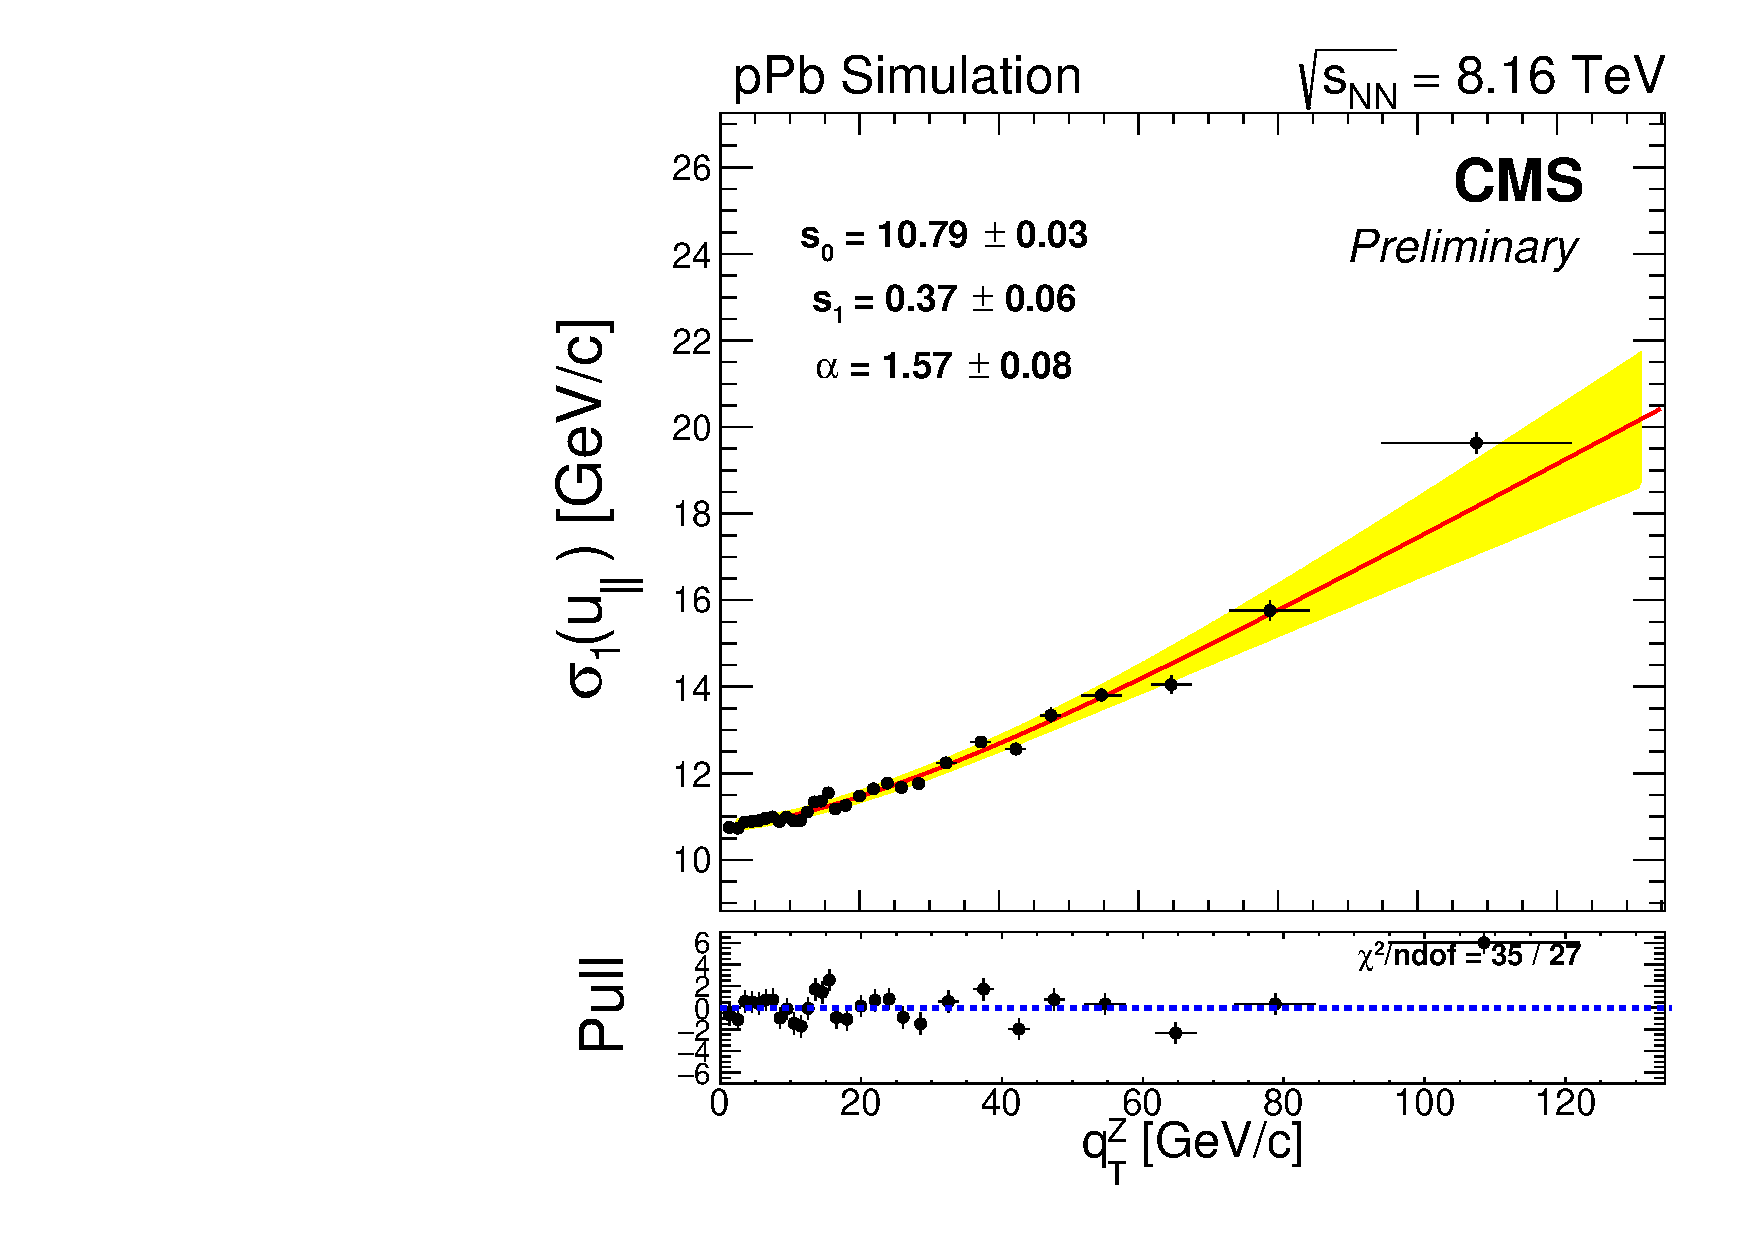
\includegraphics[width=0.3\textwidth]{Figures/WBoson/Analysis/Correction/Recoil/RecoilFitsqT/MC/fitPFu1sigma1.pdf}
  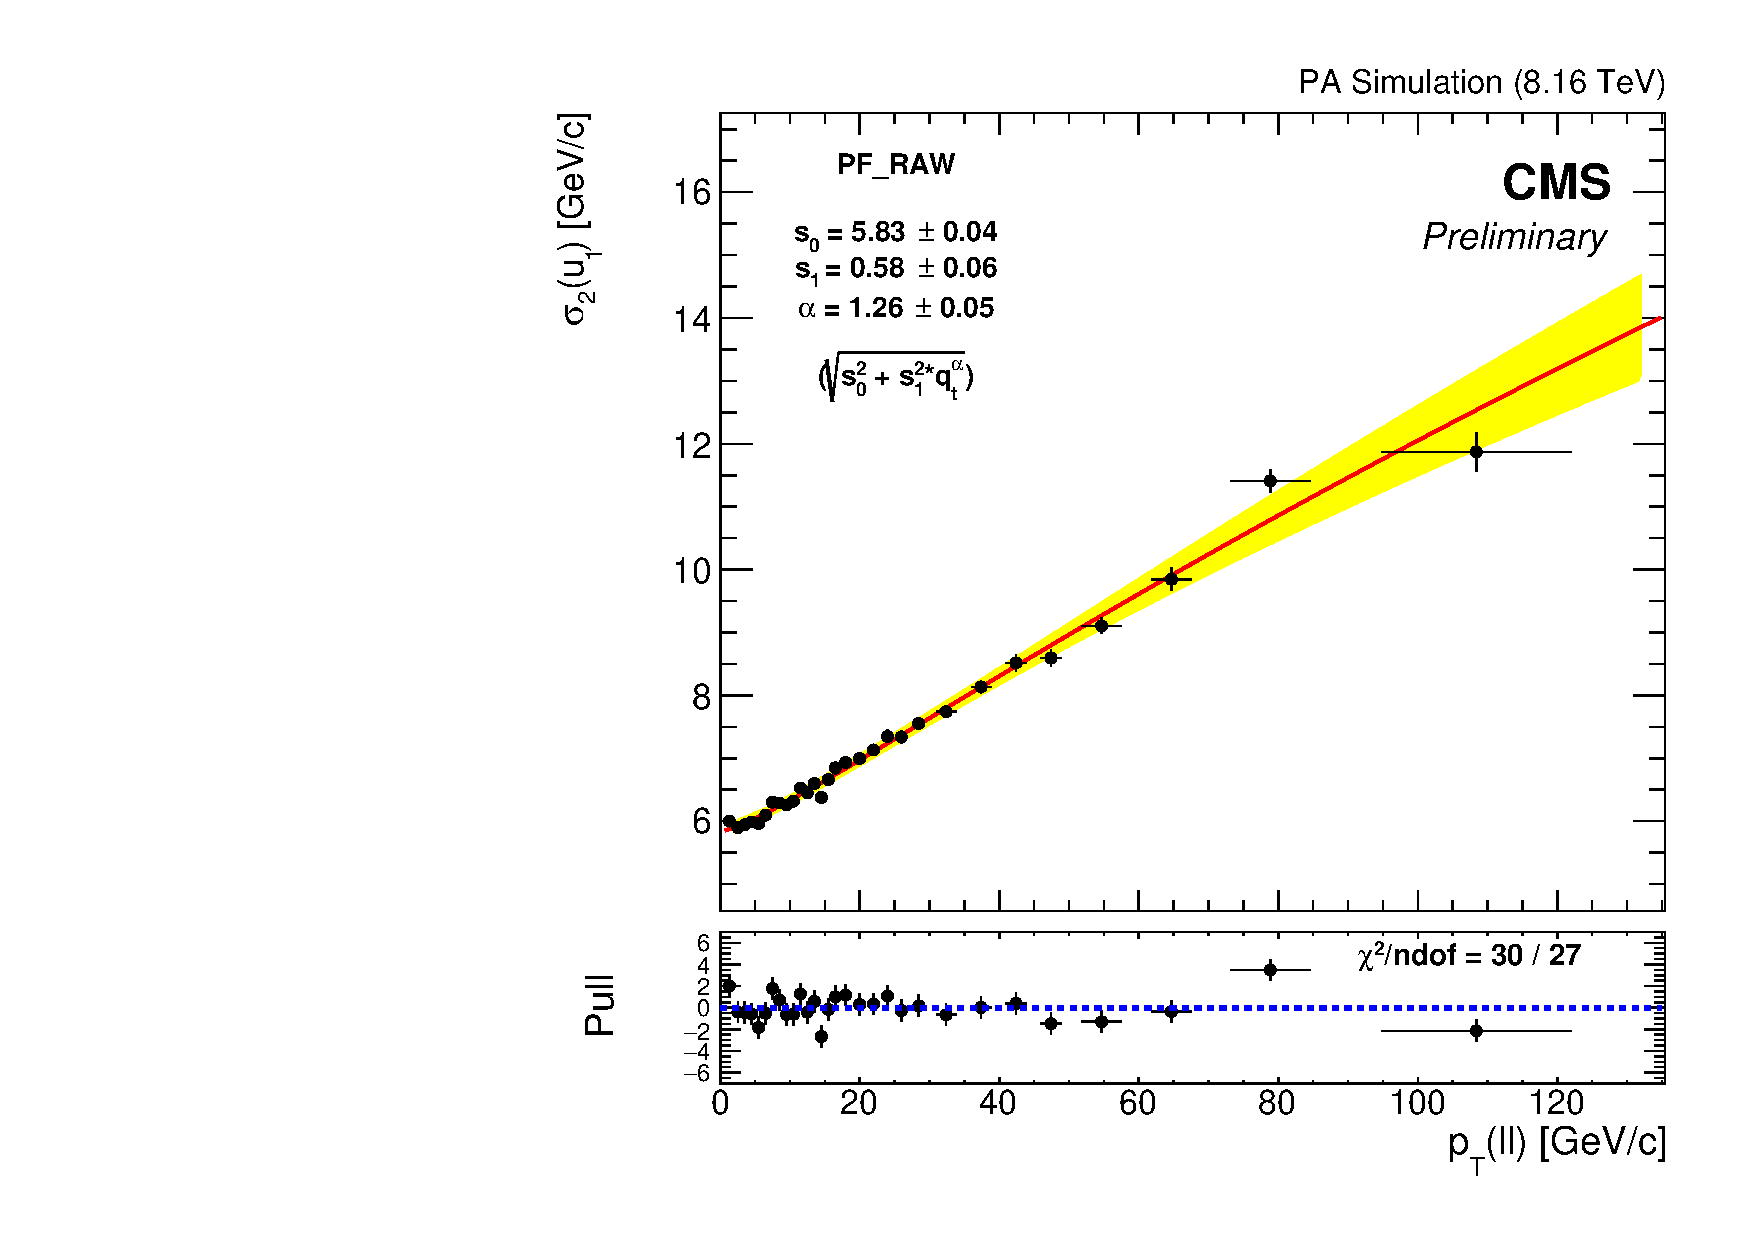
\includegraphics[width=0.3\textwidth]{Figures/WBoson/Analysis/Correction/Recoil/RecoilFitsqT/MC/fitPFu1sigma2.pdf}
  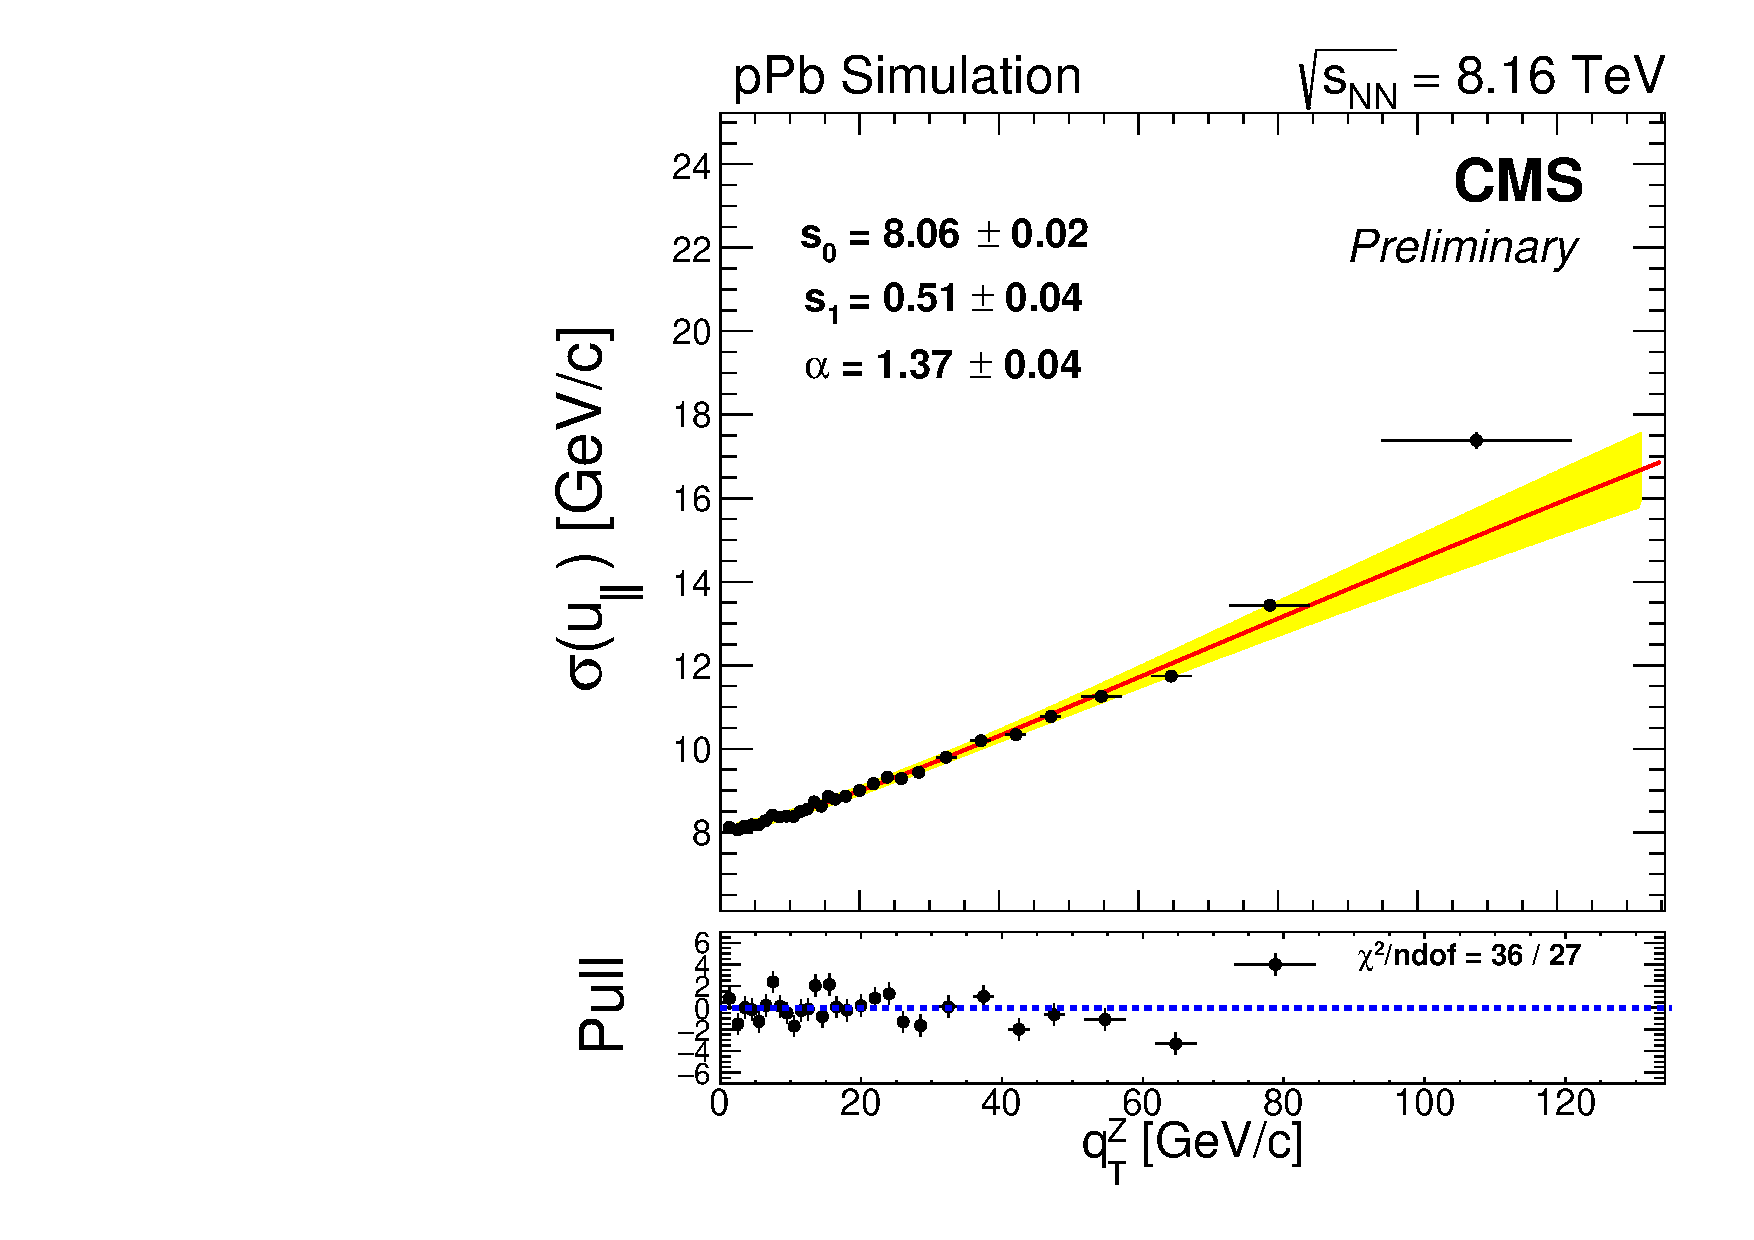
\includegraphics[width=0.3\textwidth]{Figures/WBoson/Analysis/Correction/Recoil/RecoilFitsqT/MC/fitPFu1sigma.pdf}
 \caption{Fits for the $\sigma_{1}$ (left), $\sigma_{2}$ (middle) and weighted average $\sigma$ (right) values of the parallel recoil component versus $q_{T}$. The plots on the top correspond to data while the plots in the bottom correspond to \ZToMuMu MC.}
 \label{fig:figU1RecoilResolutionFit}
 \end{center}
\end{figure}

\begin{figure} [h!]
 \begin{center}
  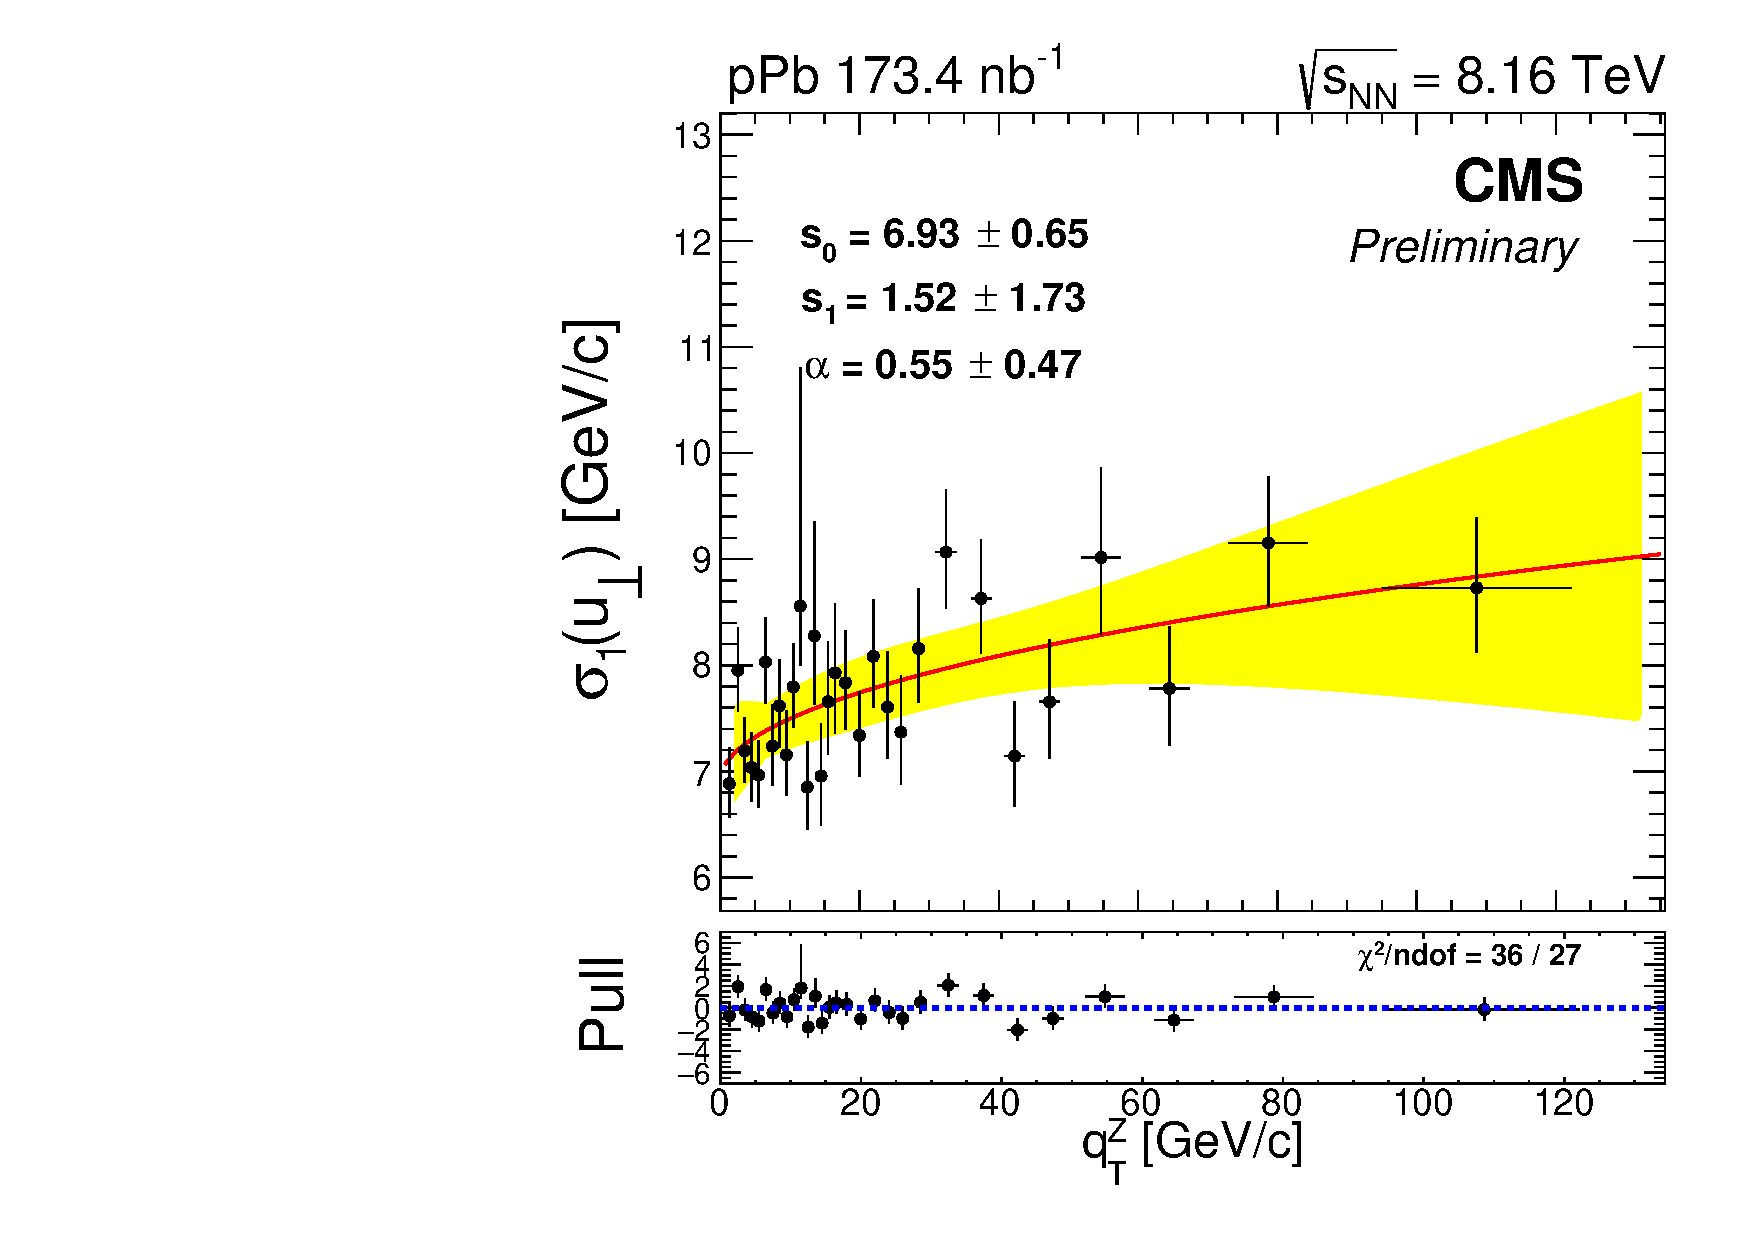
\includegraphics[width=0.3\textwidth]{Figures/WBoson/Analysis/Correction/Recoil/RecoilFitsqT/Data/fitPFu2sigma1.pdf}
  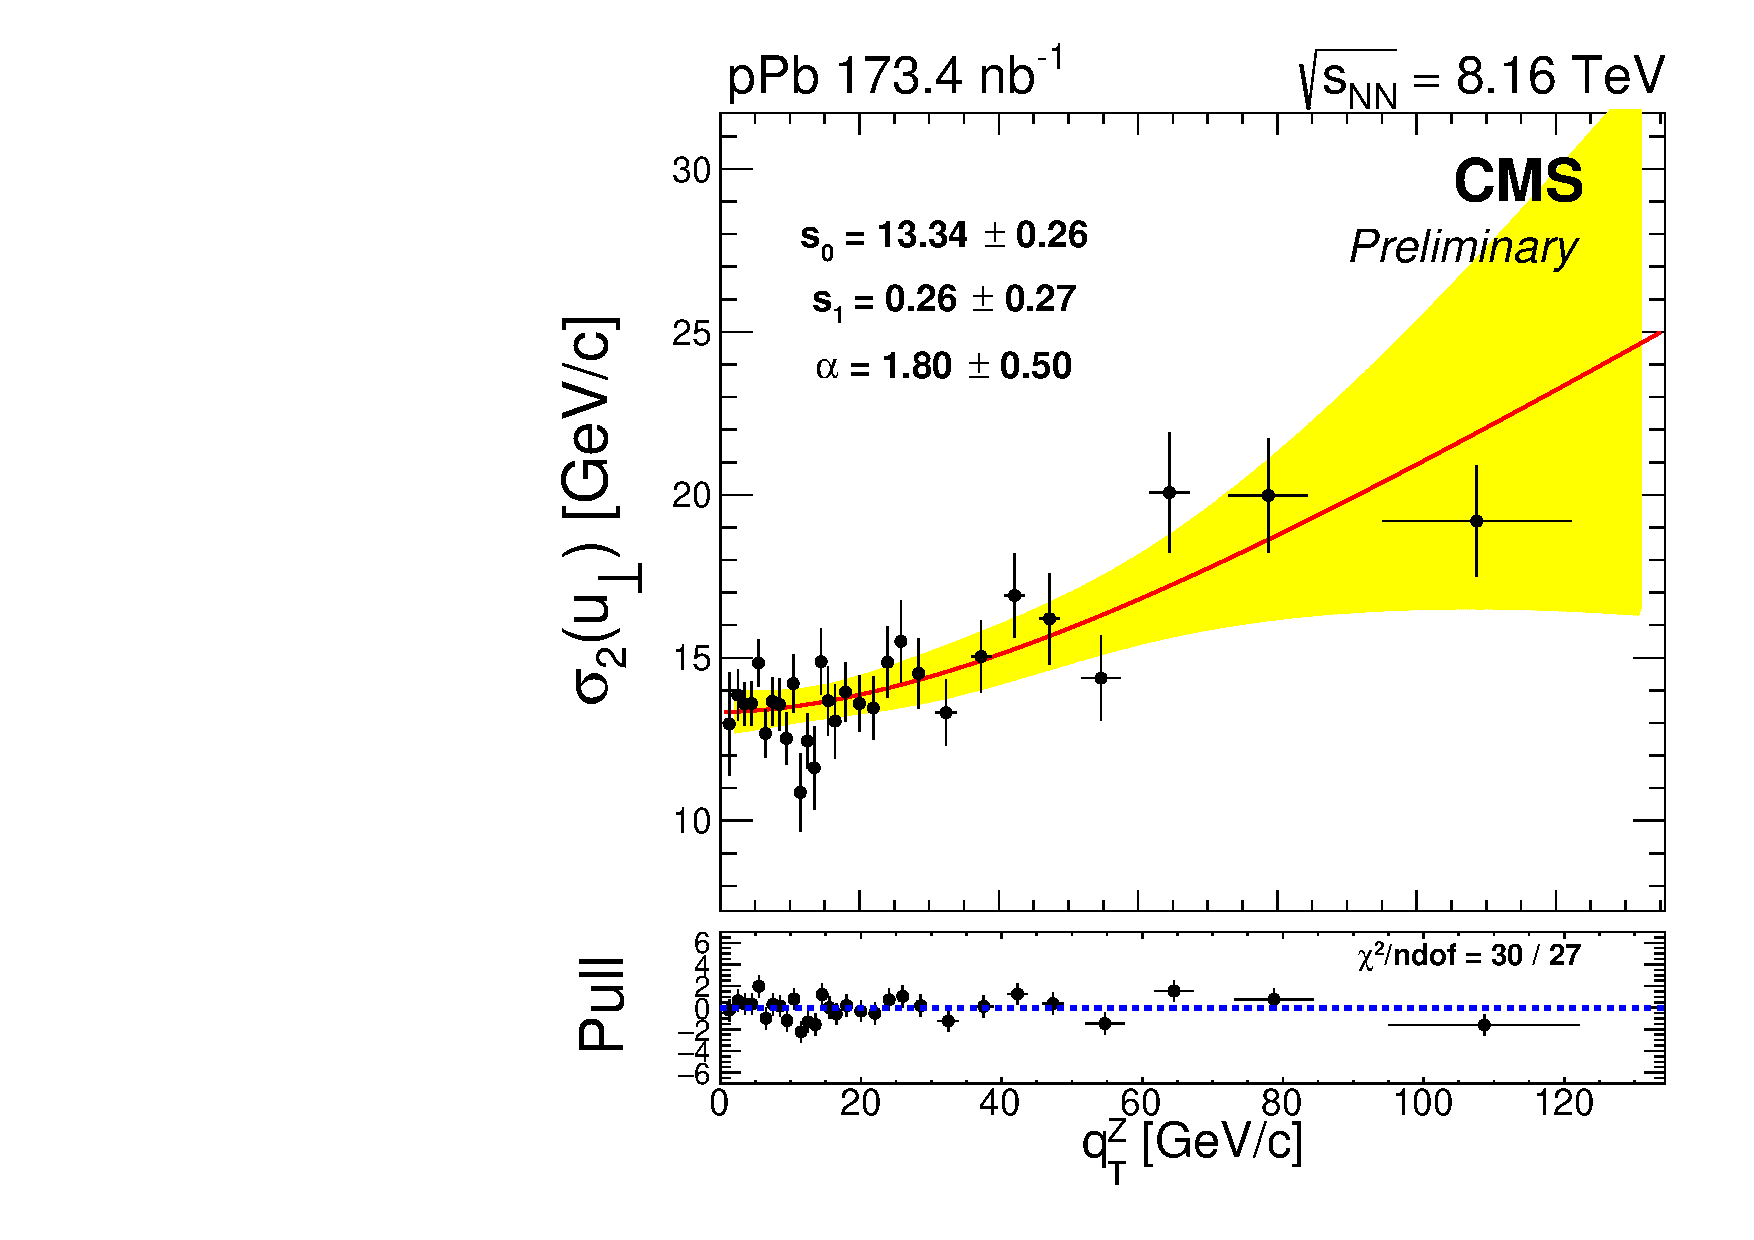
\includegraphics[width=0.3\textwidth]{Figures/WBoson/Analysis/Correction/Recoil/RecoilFitsqT/Data/fitPFu2sigma2.pdf}
  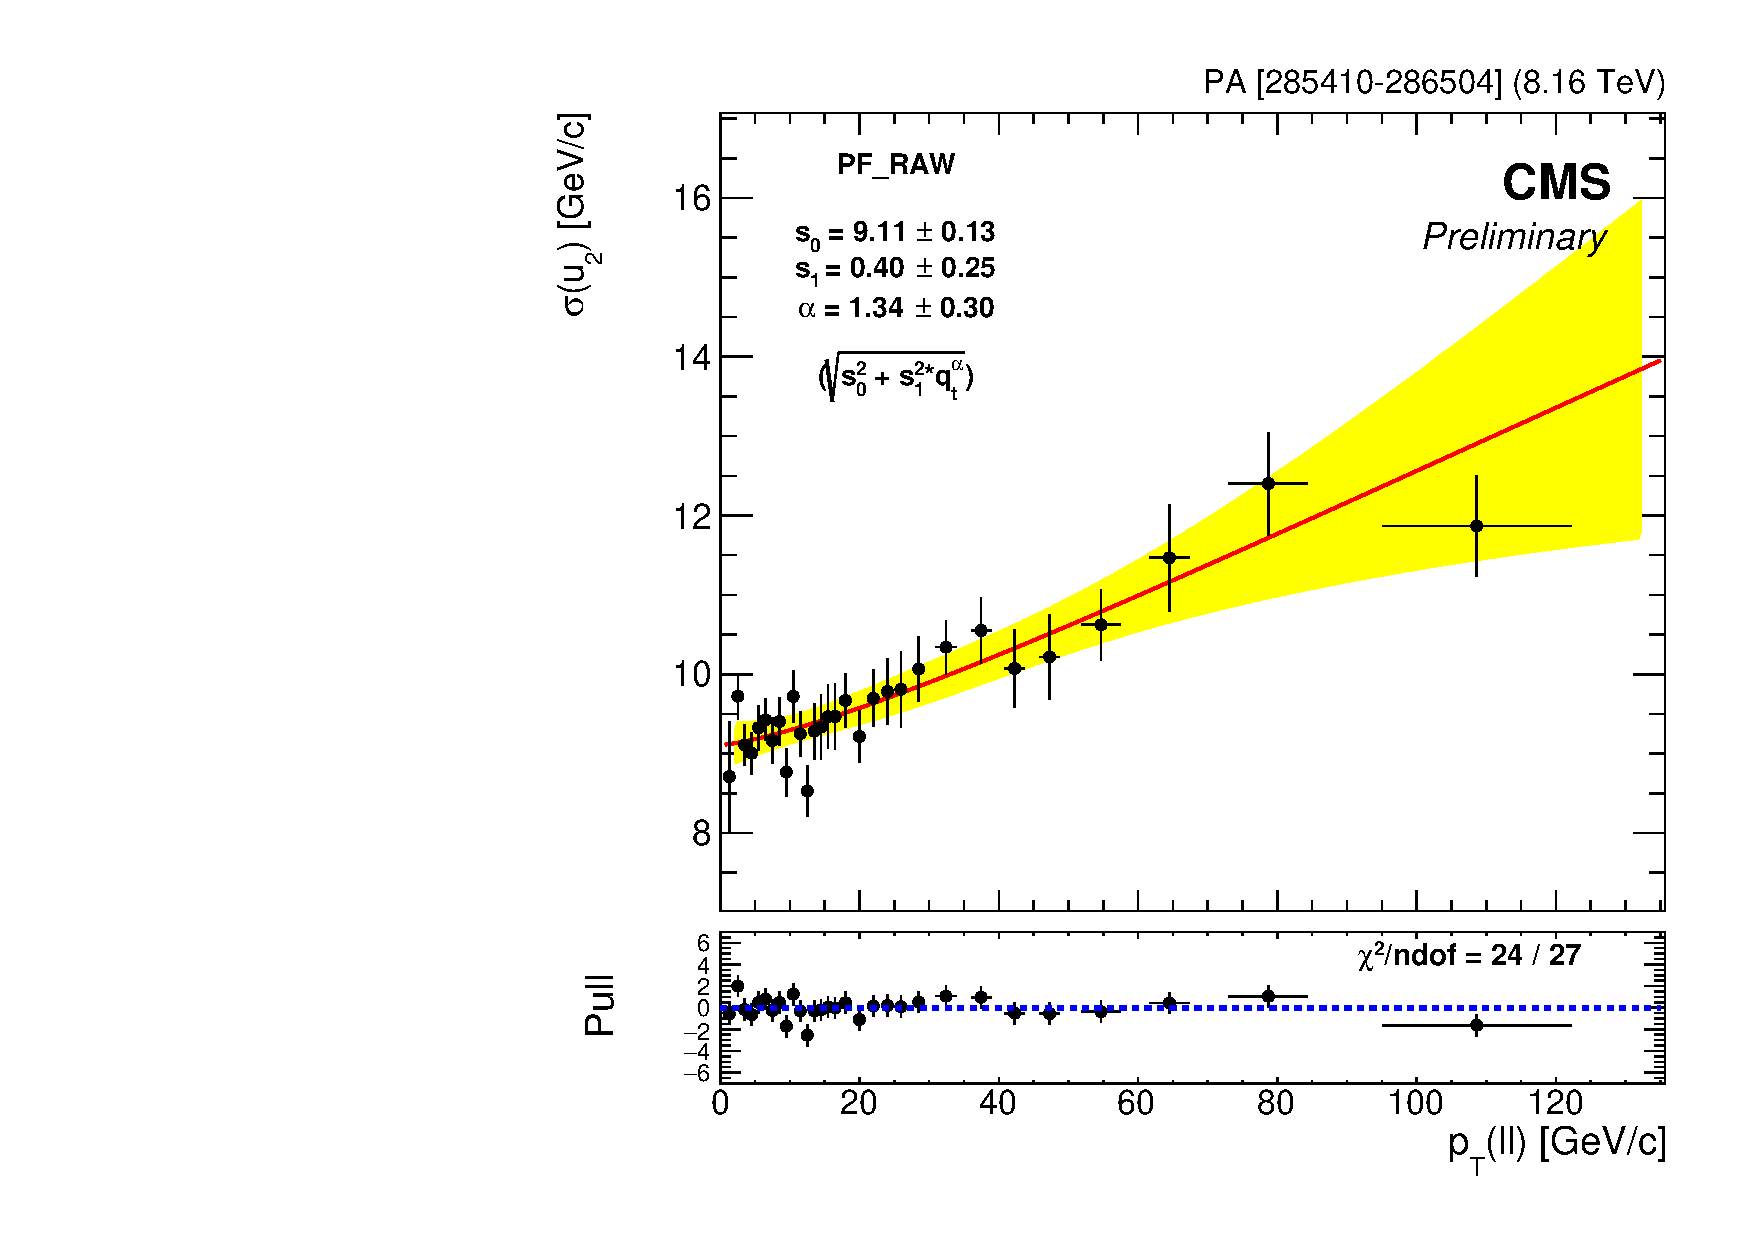
\includegraphics[width=0.3\textwidth]{Figures/WBoson/Analysis/Correction/Recoil/RecoilFitsqT/Data/fitPFu2sigma.pdf} \\
  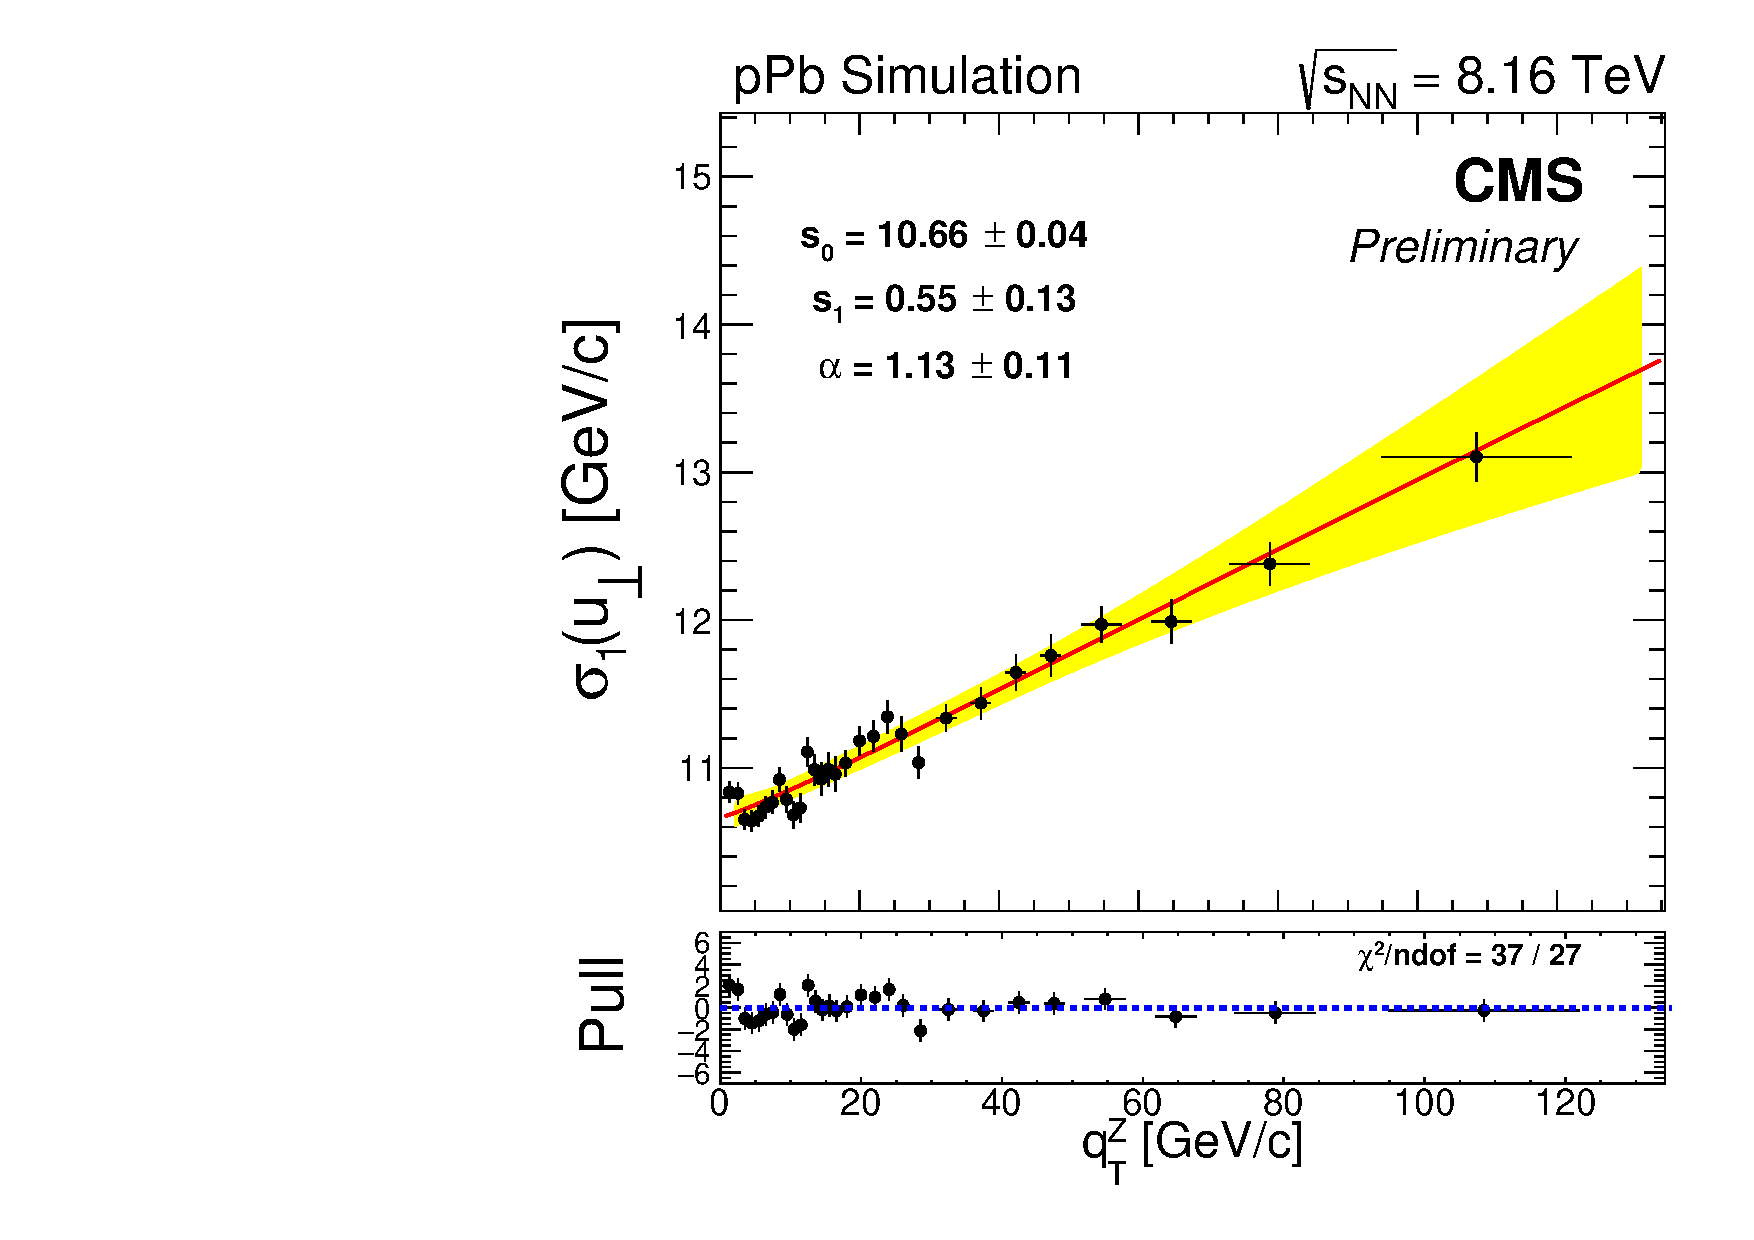
\includegraphics[width=0.3\textwidth]{Figures/WBoson/Analysis/Correction/Recoil/RecoilFitsqT/MC/fitPFu2sigma1.pdf}
  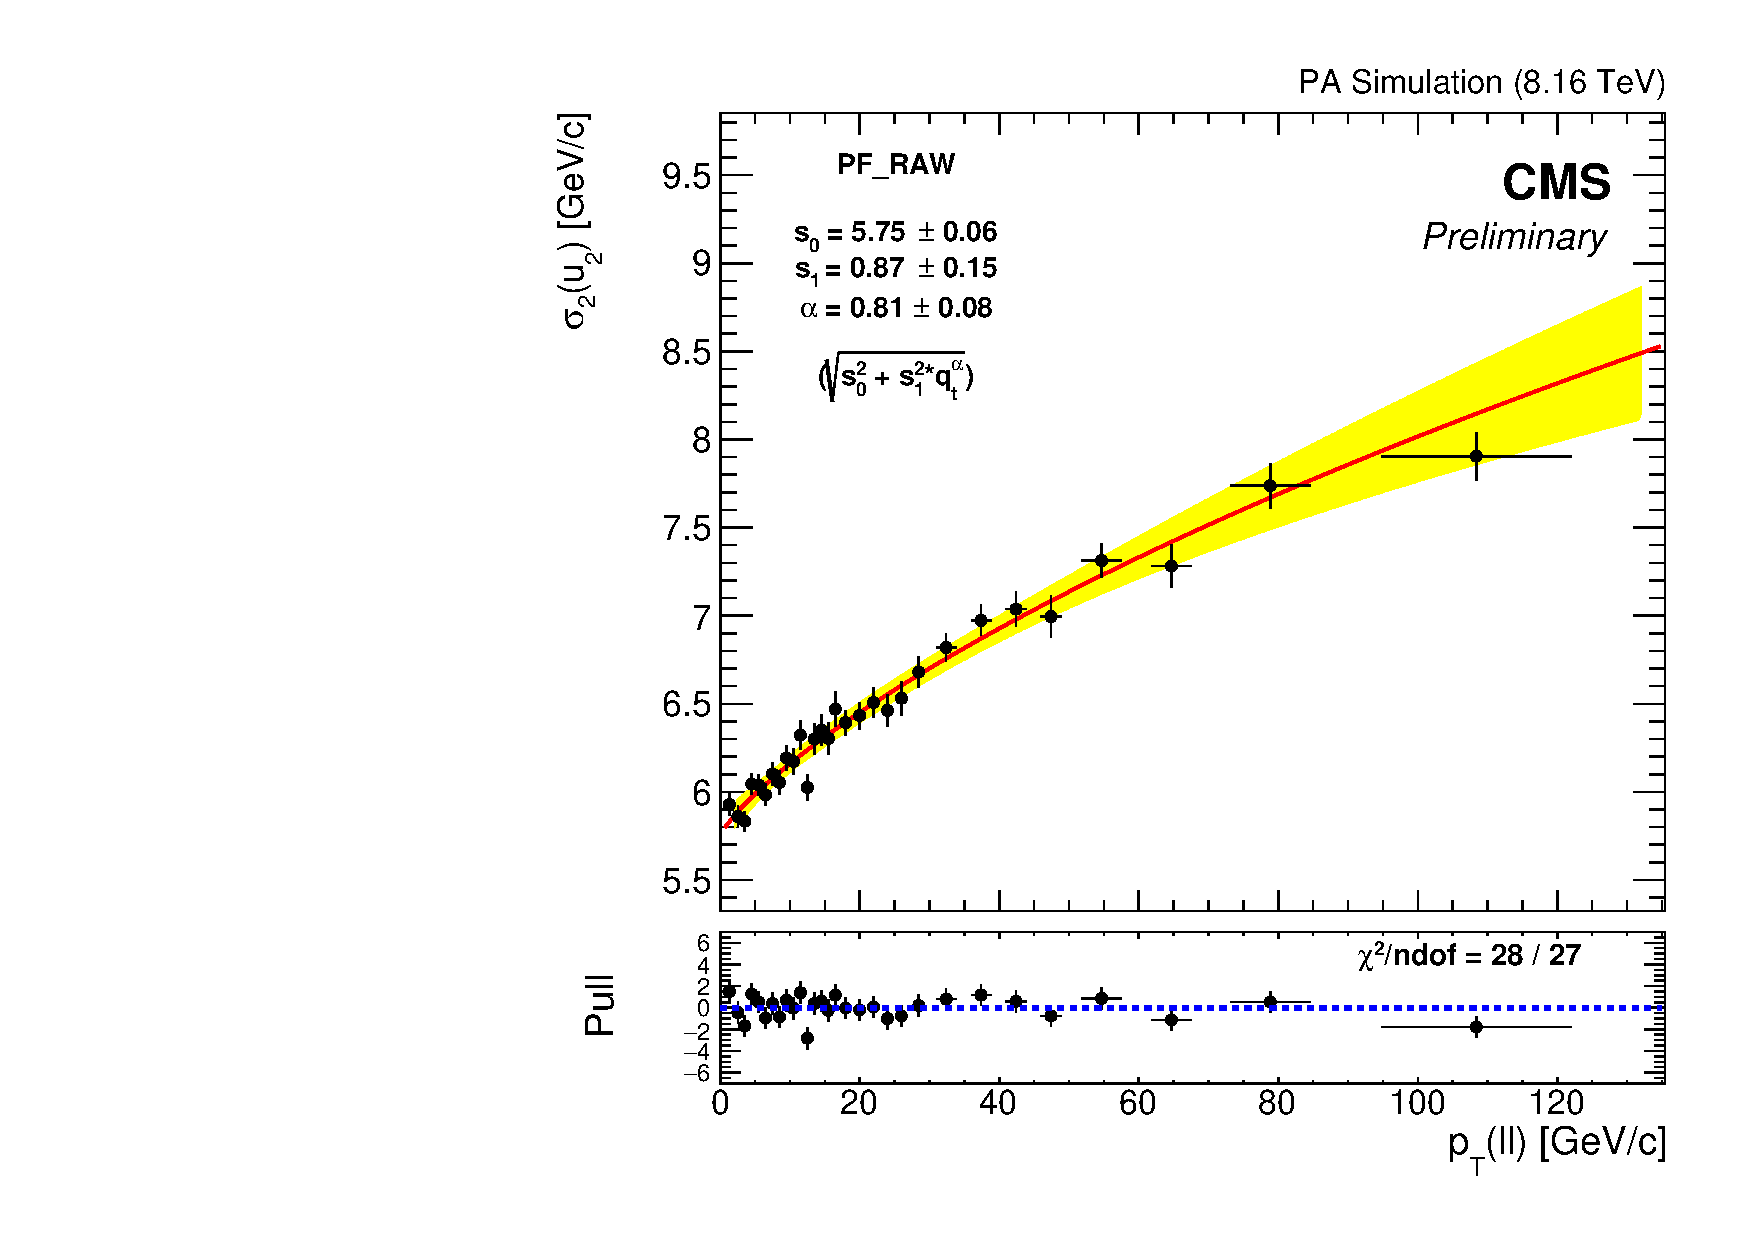
\includegraphics[width=0.3\textwidth]{Figures/WBoson/Analysis/Correction/Recoil/RecoilFitsqT/MC/fitPFu2sigma2.pdf}
  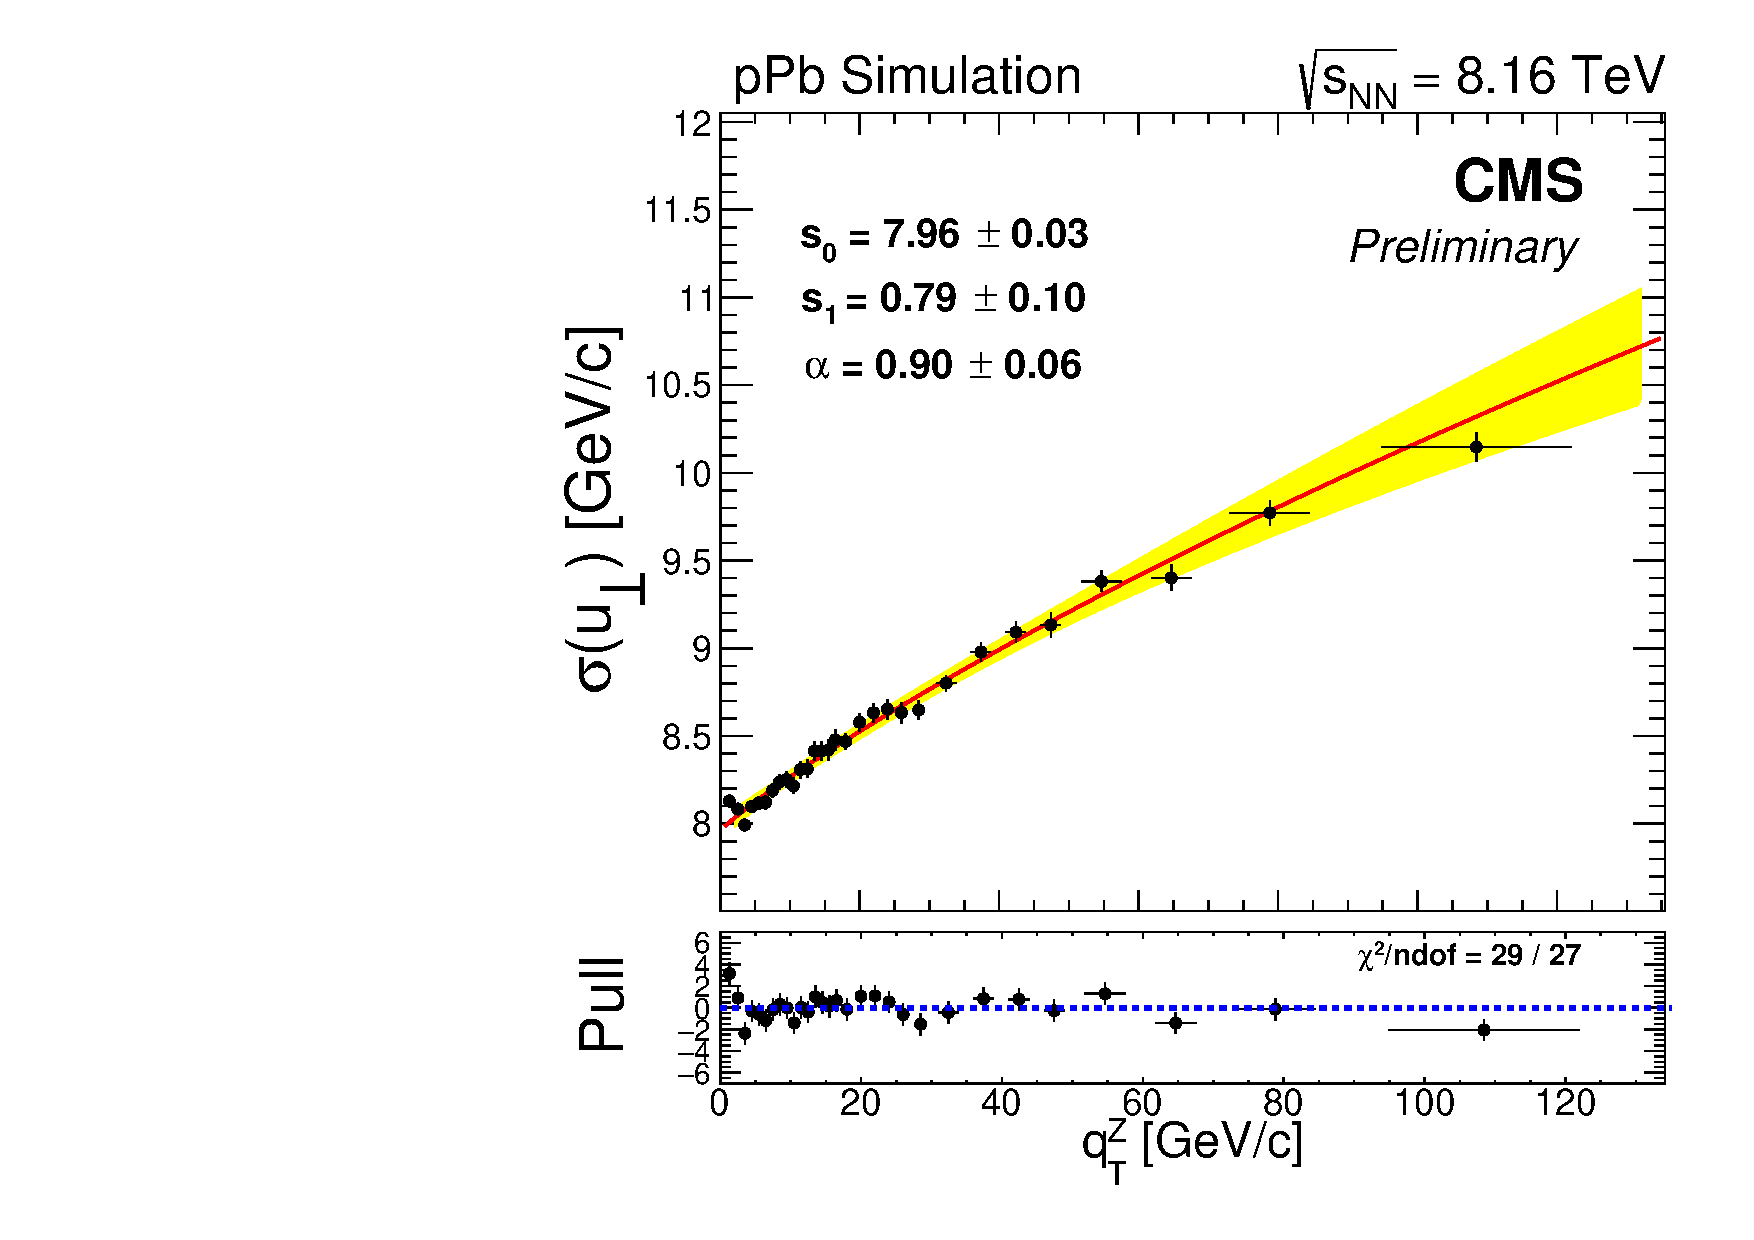
\includegraphics[width=0.3\textwidth]{Figures/WBoson/Analysis/Correction/Recoil/RecoilFitsqT/MC/fitPFu2sigma.pdf}
 \caption{Fits for the $\sigma_{1}$ (left), $\sigma_{2}$ (middle) and weighted average $\sigma$ (right) values of the recoil perpendicular component versus $q_{T}$. The plots on the top correspond to data while the plots in the bottom correspond to \ZToMuMu MC.}
 \label{fig:figU2RecoilResolutionFit}
 \end{center}
\end{figure}


\subsubsection{Recoil Correction}\label{sec:WBoson_Corrections_MET_RecoilCorr}

The simulated recoil distribution is corrected to match the scale and resolution observed in data. This can be done in two ways:

  \begin{itemize}
  \item Smearing method : Each component of the recoil distribution is smeared event-by-event using a gaussian probability distribution function defined as:
    \begin{equation}\label{eq:eqreccornsmrupar} 
%      u_{\parallel} = Gauss(u_{\parallel} - \tilde{u}_{\parallel}^{MC}(q_{T}) + \tilde{u}_{\parallel}^{data}(q_{T}), \sqrt{{\sigma_{\parallel}^{data}(q_{T},n)}^{2} - {\sigma_{\parallel}^{MC}(q_{T},n)}^{2}})
        u^{corr}_{\parallel} = Gauss(u_{\parallel} - \mu_{\parallel}^{MC}(q_{T}) + \mu_{\parallel}^{data}(q_{T}), \sqrt{{\sigma_{\parallel}^{data}(q_{T})}^{2} - {\sigma_{\parallel}^{MC}(q_{T})}^{2}}) \quad,
    \end{equation}
    \begin{equation}\label{eq:eqreccornsmruperp} 
        u^{corr}_{\perp} = Gauss(u_{\perp}, \sqrt{{\sigma_{\perp}^{data}(q_{T})}^{2} - {\sigma_{\perp}^{MC}(q_{T})}^{2}}) \quad,
    \end{equation}
    
    where $\mu$ and $\sigma$ are the weighted average values obtained in the previous subsections.
    
    \item Scaling method :  The parallel and perpendicular components of the simulated recoil are scaled in two possible ways:
    
      \begin{itemize}
       \item General case: Considering the full information of the double gaussian PDF used to fit the recoil distributions in data and MC, by using their Cumulative Distribution Functions (CDF).
       \begin{equation}\label{eq:eqRecCorrGeneralCase} 
         u^{corr}_{\parallel, \perp} = CDF^{-1}_{data}[CDF_{MC}[u_{\parallel, \perp}^{MC}]]
       \end{equation}
       
       \item Gaussian case: Approximating the recoil distributions by assuming a single gaussian PDF using the weighted average values $\mu$ and $\sigma$ derived before.
       \begin{equation}\label{eq:eqreccornsclupar} 
         u^{corr}_{\parallel} = (u_{\parallel} - \mu_{\parallel}^{MC}(q_{T}))\frac{\sigma_{\parallel}^{data}(q_{T})}{\sigma_{\parallel}^{MC}(q_{T})} + \mu_{\parallel}^{data}(q_{T}),
       \end{equation}
       \begin{equation}\label{eq:eqreccornscluperp} 
         u^{corr}_{\perp} = u_{\perp}\frac{\mu_{\perp}^{data}(q_{T})}{\sigma_{\perp}^{MC}(q_{T})}
       \end{equation}
      \end{itemize}

  \end{itemize}

Once the recoil is corrected, the MET distribution is recalculated as:

\begin{equation}
 \textsc{MET}_{corr} = \left|\vec{p}^{\mu}_{T} + \vec{u}_{corr}\right|
\end{equation}


\subsubsection{Recoil Correction: Control Region}\label{sec:WBoson_Corrections_MET_closureTests}

The recoil corrections are checked by applying them on the same MC sample used to derive the recoil corrections (Z boson enriched). The data and simulation (including HF reweighing) corrected MET distributions are shown in \fig{fig:recoilClosure} in the inclusive (left) and in a selected (right) pseudorapidity region. As can be observed, the  agreement between simulation and data is greatly improved after applying the recoil correction using the gaussian scaling method.

\begin{figure}[!h]
 \begin{center}
  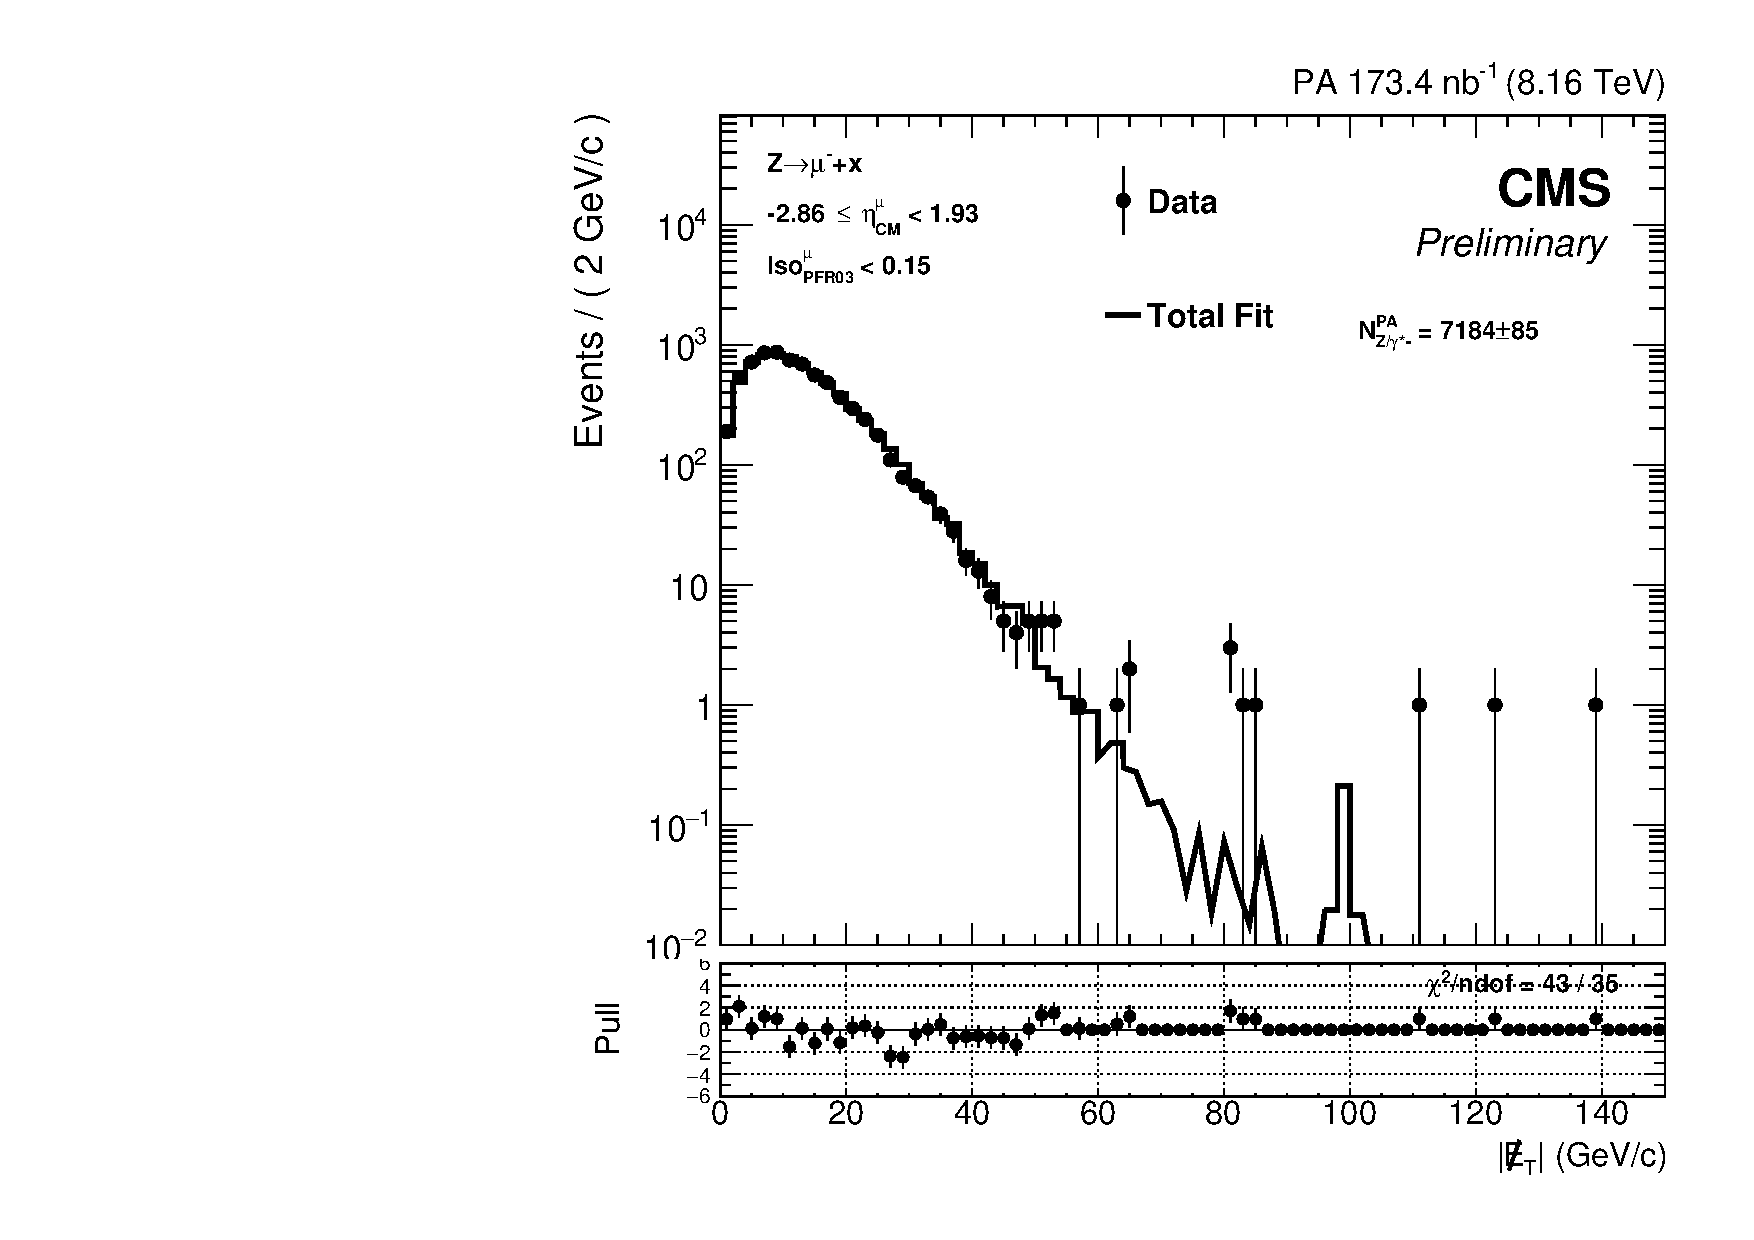
\includegraphics[width=0.4\textwidth]{Figures/WBoson/Analysis/Correction/Recoil/CheckFits/Z/Recoil_ScalingGauss/PLOT_MET_DATA_ZToMuMi_PA_Model_TEMP_DY_MuEtaCM_m286_193_MuIso_0_15.pdf}
  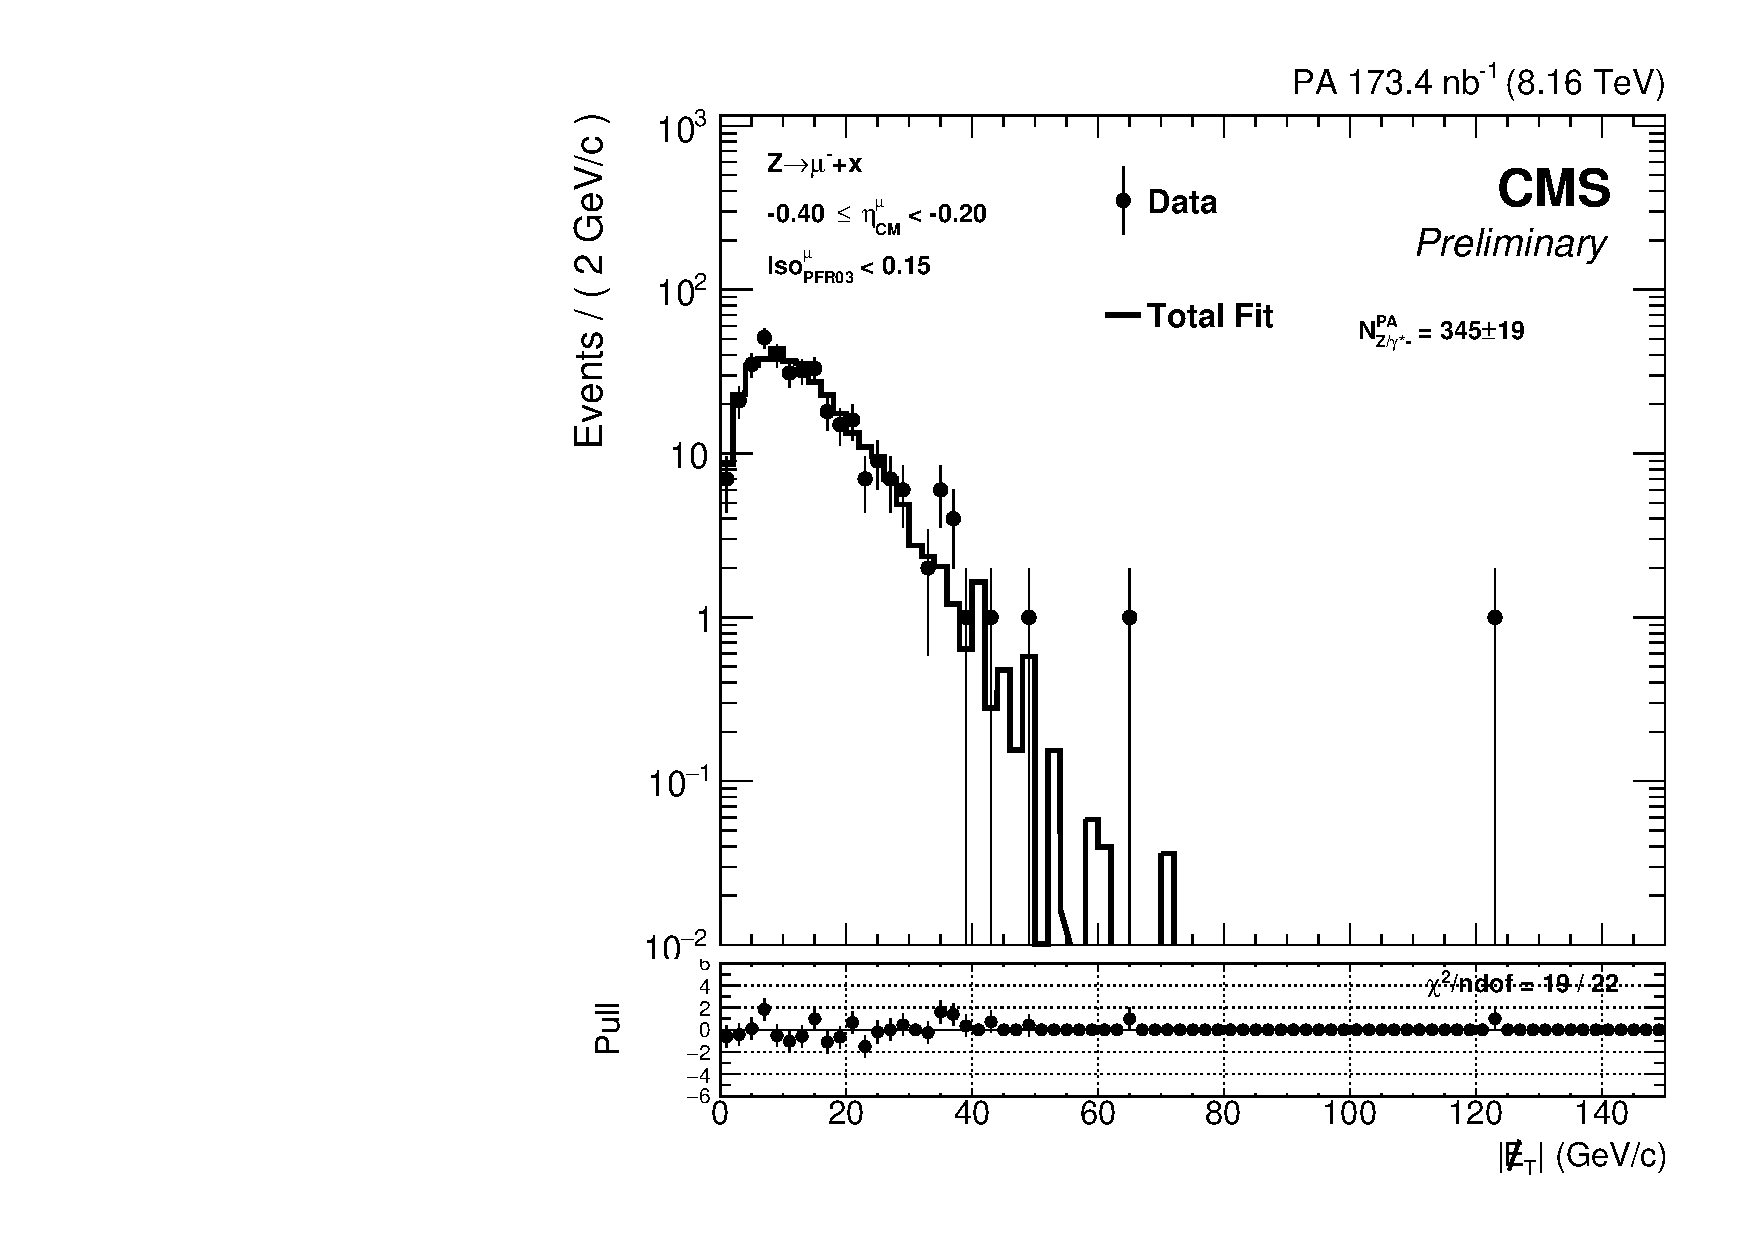
\includegraphics[width=0.4\textwidth]{Figures/WBoson/Analysis/Correction/Recoil/CheckFits/Z/Recoil_ScalingGauss/PLOT_MET_DATA_ZToMuMi_PA_Model_TEMP_DY_MuEtaCM_m40_m20_MuIso_0_15.pdf} 
  \caption{A comparison of the MET distribution in data and MC for Z boson selected events. The left plot corresponds to the full pseudorapidity range in the analysis while the right one corresponds to an pecific pseudorapidity bin. The recoil correction using the gaussian scaling method has been applied to MC.}
 \label{fig:recoilClosure}
 \end{center}
\end{figure}

\subsubsection{Recoil Correction: Signal Region}\label{sec:WBoson_Corrections_MET_RecoilSignal}

The \W signal in data is extracted following the procedure in \sect{sec:WBoson_SignalExtraction}. The recoil corrections are applied to the \W boson MC using the 3 methods detailed in \sect{sec:WBoson_Corrections_MET_RecoilCorr}, in order to determine which one works better. \fig{fig:recoilCorrWreg} shows the data fits in the \W region with the scaling method in the general case (left), gaussian case (middle) and the smearing method (right), for the full pseudorapidity region used in the analysis. The gaussian scaling provides the best fits, so it is used as nominal correction method.

\begin{figure}[!h]
 \begin{center}
  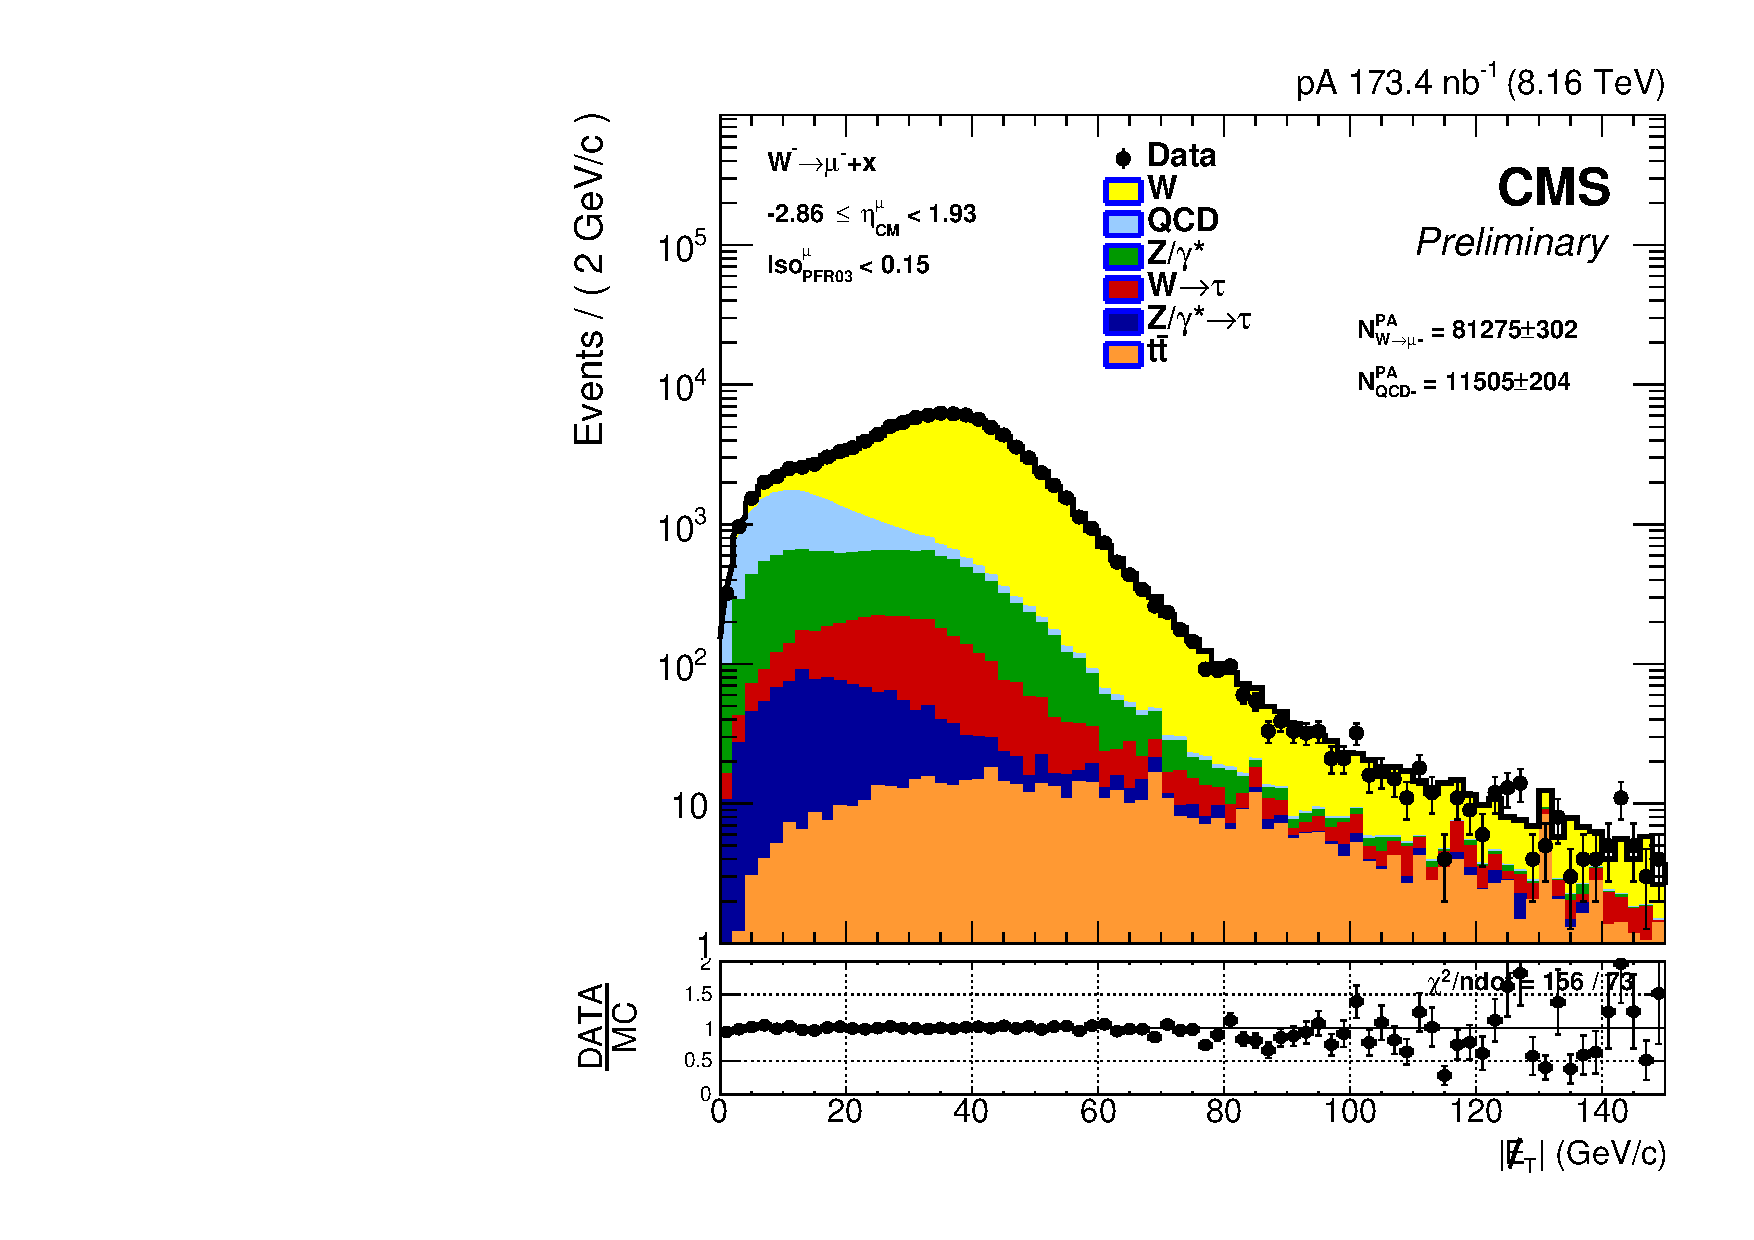
\includegraphics[width=0.3\textwidth]{Figures/WBoson/Analysis/Correction/Recoil/CheckFits/W/Recoil_ScalingGeneral/PLOT_MET_DATA_WToMuMi_PA_Model_TEMP_WDYDYToTauWToTauTTbar_ModifiedRayleigh_QCD_MuEtaCM_m286_193_MuIso_0_15.pdf}
  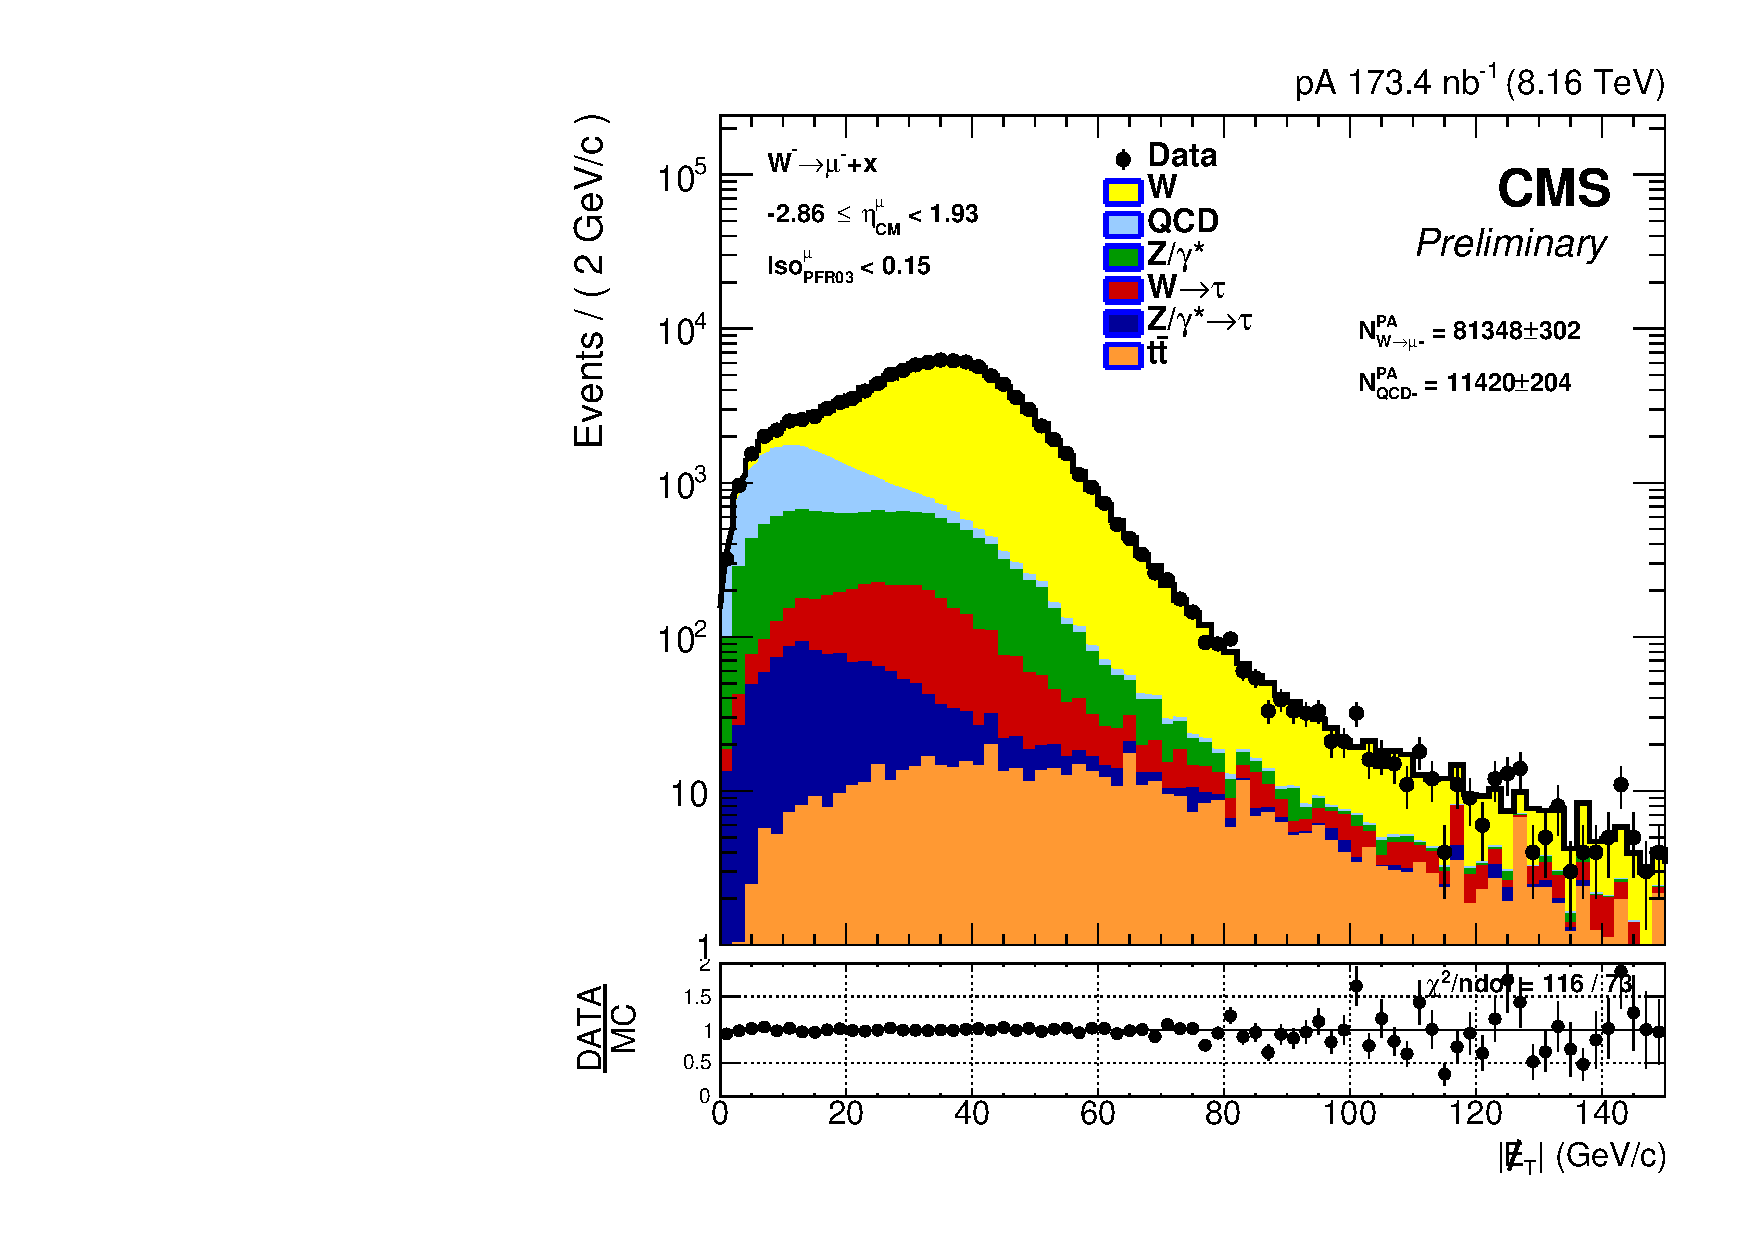
\includegraphics[width=0.3\textwidth]{Figures/WBoson/Analysis/Correction/Recoil/CheckFits/W/Recoil_ScalingGauss/PLOT_MET_DATA_WToMuMi_PA_Model_TEMP_WDYDYToTauWToTauTTbar_ModifiedRayleigh_QCD_MuEtaCM_m286_193_MuIso_0_15.pdf}
  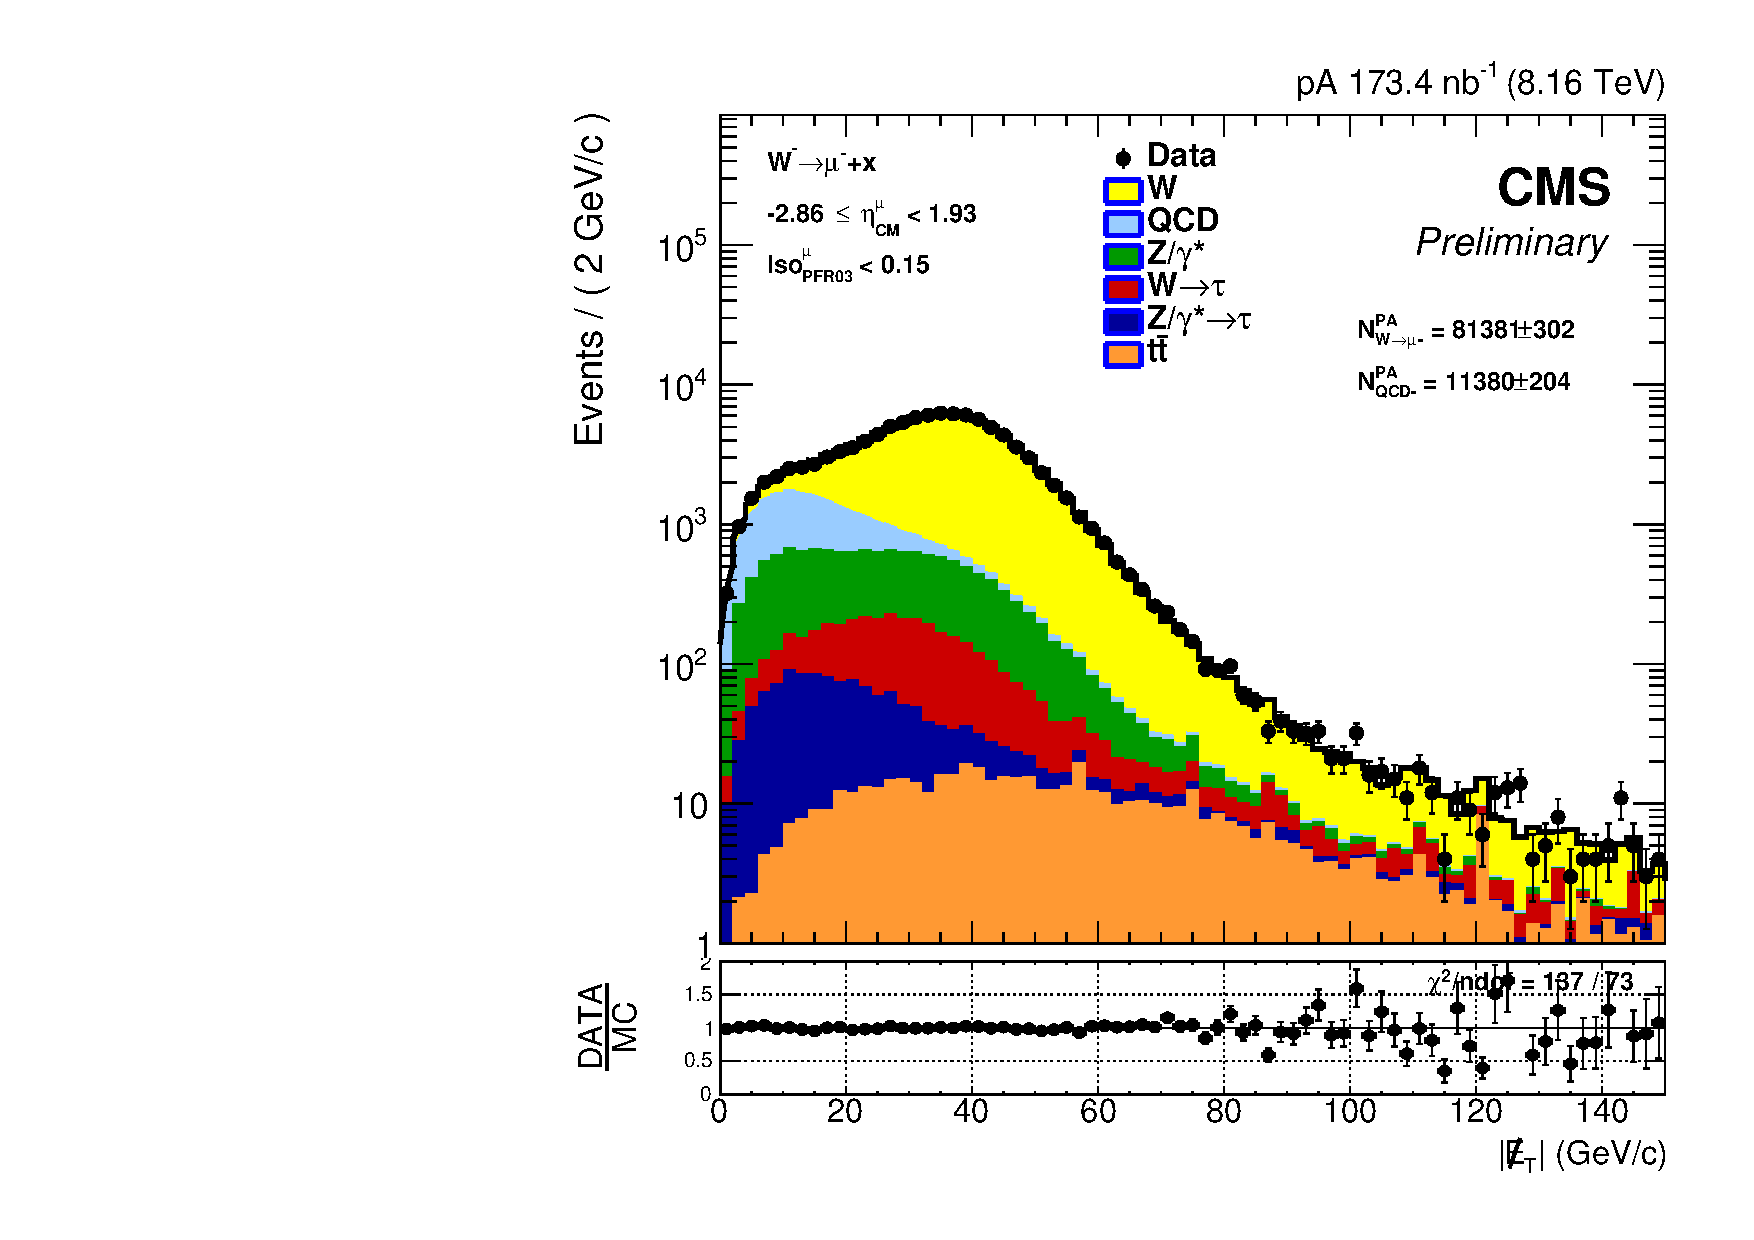
\includegraphics[width=0.3\textwidth]{Figures/WBoson/Analysis/Correction/Recoil/CheckFits/W/Recoil_Smearing/PLOT_MET_DATA_WToMuMi_PA_Model_TEMP_WDYDYToTauWToTauTTbar_ModifiedRayleigh_QCD_MuEtaCM_m286_193_MuIso_0_15.pdf}
  \caption{A comparison of the MET distribution in data and MC for W boson selected events in the full pseudorapidity range in the analysis. Different methods to apply the recoil corrections in MC are used in each plot. The left plot corresponds to the scaling method in the general case, the middle one corresponds to the scaling method in the gaussian case, and the right one to the smearing method.}
 \end{center}
 \label{fig:recoilCorrWreg}
\end{figure}


% END OF SUBSECTION
